% =====================================================================
% IT8105 Machine Learning -- Assessment 2 Final Report
% Samina Tuladhar (20251674)
% Compile: pdflatex main -> bibtex main -> pdflatex main -> pdflatex main
% (or latexmk -pdf main). Figures are in ./figures, references in references.bib
% =====================================================================
\documentclass[11pt,a4paper]{report}

\usepackage[T1]{fontenc}
\usepackage[utf8]{inputenc}
\usepackage{lmodern}
\usepackage[margin=2.5cm]{geometry}
\usepackage{amsmath,amssymb}
\usepackage{graphicx}
\usepackage{booktabs}
\usepackage{tabularx}
\usepackage{longtable}
\usepackage{array}
\usepackage{multirow}
\usepackage[table]{xcolor}
\usepackage{caption}
\usepackage{float}
\usepackage{enumitem}
\usepackage{setspace}
\usepackage{titlesec}
\usepackage[natbibapa]{apacite}
\usepackage[hyphens]{url}
\makeatletter\g@addto@macro\UrlBreaks{\do\_\do\-}\makeatother
\usepackage[hidelinks]{hyperref}
\usepackage{fvextra}

\graphicspath{{figures/}}
\setstretch{1.2}
\setlength{\parskip}{4pt}
\captionsetup{font=small,labelfont=bf}
\setlist{itemsep=2pt,topsep=3pt}
\newcolumntype{L}[1]{>{\raggedright\arraybackslash}p{#1}}
\newcolumntype{Y}{>{\raggedright\arraybackslash}X}
\renewcommand{\arraystretch}{1.15}

% Template-style chapter headings: "Chapter 1. Introduction"
\titleformat{\chapter}[hang]{\normalfont\LARGE\bfseries}{Chapter \thechapter.}{0.5em}{}
\titlespacing*{\chapter}{0pt}{0pt}{14pt}
\renewcommand{\thesection}{\thechapter.\arabic{section}}
\renewcommand{\thesubsection}{\thechapter.\arabic{section}.\arabic{subsection}}
\titleformat{\section}{\normalfont\Large\bfseries}{\thesection.}{0.5em}{}
\titleformat{\subsection}{\normalfont\large\bfseries}{\thesubsection.}{0.5em}{}
\titlespacing*{\section}{0pt}{3.5ex plus 1ex minus .2ex}{2.3ex plus .2ex}
\titlespacing*{\subsection}{0pt}{3.25ex plus 1ex minus .2ex}{1.5ex plus .2ex}

\setlength{\emergencystretch}{3em}

\begin{document}

% ----------------------------------------------------------------- title page
\hypersetup{pageanchor=false}
\begin{titlepage}
\centering
\vspace*{1.5cm}
{\Large\bfseries IT8105 Machine Learning\par}
\vspace{0.4cm}
{\large\bfseries Final Report\par}
\vspace{2.5cm}
{\LARGE\bfseries Area-Level Crime Hotspot and\\[4pt] High-Victimisation Risk Prediction\par}
\vspace{2.5cm}
{\large
\begin{tabular}{lcl}
Student Name & : & Samina Tuladhar\\
Student ID   & : & 20251674\\
Lecturer     & : & Dr Joseph Dang\\
\end{tabular}\par}
\vfill
{\large A document submitted to Whitecliffe in partial fulfilment of the requirements for the course of IT8105 Machine Learning\par}
\vspace{1cm}
{\large Whitecliffe\\ 2026\par}
\vspace{1cm}
{\large Submission Date: [insert submission date]\par}
\end{titlepage}

\hypersetup{pageanchor=true}
\pagenumbering{roman}

% ----------------------------------------------------------------- abstract
\chapter*{Abstract}
\addcontentsline{toc}{chapter}{Abstract}
Recorded crime in the City of Chicago is highly clustered, with the busiest 20\% of 2.2 km grid cells accounting for approximately half of all recorded incidents. This study evaluates whether an area-level forecasting approach using a Spatial Graph Convolutional Network (GCN) can achieve more accurate predictions for the two forecasting tasks: (1) dominant crime type during the following 28 days and (2) whether a cell is among the top 20\% for recorded victimisation-related incidents, versus persistence, kernel density, logistic regression (LR), SVM, random forest, MLP, and graph-attention baselines. Features use only past periods; models are tuned using validation periods and tested in chronological order using ten seeds, spatial-block bootstrap intervals, and permutation testing. A review found that the label for Phase 1 of the Assessment 1 pilot was present in its features, and LR matched the pilot's Phase 2 result. For one year (228,595 rows, 157 cells), LR achieved an average precision of 0.983 and macro-F1 of 0.951 for cells with high victimisation, exceeding the pre-registered criterion of 0.70, but persistence achieved 0.973 and no learned model performed significantly better than persistence. The GCN reached 0.885 and a residual variant 0.975; neither made use of neighbouring cells productively, and a three-year replication (732,017 rows, six test periods) yielded the same ranking. Predicting the dominant crime type remained difficult (highest macro-F1 around 0.50). A tested API prototype reproduces the offline results exactly. A transparent model with a human-in-the-loop approach is recommended.


\tableofcontents
\listoffigures
\listoftables

\chapter*{List of Abbreviations}
\addcontentsline{toc}{chapter}{List of Abbreviations}
\begin{center}
\small
\resizebox{\textwidth}{!}{\begin{tabular}{@{}ll@{\hspace{1.2cm}}ll@{}}
\toprule
\textbf{Abbreviation} & \textbf{Meaning} & \textbf{Abbreviation} & \textbf{Meaning}\\
\midrule
AP & Average precision (step-wise PR-AUC) & MLP & Multilayer perceptron\\
AUC & Area under the ROC curve & PAI & Predictive Accuracy Index\\
CI & Confidence interval & PR & Precision--recall\\
CPD & Chicago Police Department & RBF & Radial basis function\\
DBSCAN & Density-based spatial clustering & ResGCN & GCN with residual self path\\
GCN & Graph convolutional network & RF & Random forest\\
KDE & Kernel density estimation & RO / RQ & Research objective / question\\
LO & Course learning outcome & SMOTE & Synthetic minority over-sampling\\
LR & Logistic regression & SVM & Support vector machine\\
GAT & Graph attention network & MAE, RMSE & Mean absolute / root mean square error\\
\bottomrule
\end{tabular}}
\end{center}

\clearpage
\pagenumbering{arabic}

% =====================================================================
\chapter{Introduction}
\label{ch:intro}
The purpose of this chapter is to restate the research problem as presented in Assessment~1, outline how the problem was refined through the pilot audit process, and define the research objectives, research questions, and report structure

\section{Problem Statement}
Crime is not evenly distributed across a city. A small number of locations account for a substantial proportion of recorded incidents, and this pattern is sufficiently stable to inform planning \citep{weisburd2015}. Police and community-safety agencies therefore seek to identify \emph{where} recorded harm is likely to be concentrated during the next planning period and \emph{which type} of crime is likely to predominate in those locations. Traditional hotspot mapping techniques like kernel density estimation (KDE) provide information about locations where past incidents clustered \citep{chainey2008}. Machine-learning classifiers can incorporate multiple historical features but treat areas as independent observations. GCNs represent areas as nodes of a spatial graph, allowing each prediction to draw on information from neighbouring areas  \citep{kipf2017,zubair2025}.

In Assessment 1, a two-step approach was proposed using the CPD dataset aggregated in 2.2~km $\times$ 2.2~km cells. Phase~1 involved predicting the predominant crime category in each cell by a GCN and an SVM baseline; Phase~2 involved predicting whether a cell would have high victimisation in the future by a GCN and an LR baseline. The pilot audit of this process prior to conducting the final experiment (Section~\ref{sec:audit}) uncovered three issues that altered the scope:

\begin{enumerate}
\item the Phase~1 features consisted of the same-period crime-type counts whose maximum \emph{is} the label, and hence the task was circular;
\item Phase~2 involved one split between historical and future data with a random 24-cell test set, and hence did not evaluate forecasting into a new period; and
\item a plain LR, as well as a persistence strategy, perfectly replicated the pilot's Phase~2 results on the same split.
\end{enumerate}
The final study thus reformulates both phases as proper one-period-ahead forecasts, employing leakage-free features, matched baselines and chronological testing.

\paragraph{Operational definitions.} 
The prediction unit is a 2.2 km grid cell, and forecasts cover the next 28-day period. The  \emph{dominant crime type} is the most frequently recorded primary crime category within a given cell and period; it describes the composition of recorded offending rather than hotspot intensity. \emph{High recorded victimisation} means that a cell ranks among the top 20\%  of cells for that period based on its count of person-directed incidents: assault, battery, robbery, criminal sexual assault, sex offence, stalking, homicide, kidnapping, offences involving children, intimidation and human trafficking. These figures count recorded incidents rather than unique victims and are not adjusted for population size. They should therefore not be interpreted as an individual's probability of becoming a victim. The intended users are crime and community-safety analysts developing area-level prevention strategies. The outputs support decision-making and do not provide instructions for automated deployment.

Formally, for cell  $i$ in period $t$, with features $\mathbf{x}_{i,t}$ derived only from earlier periods and graph neighbours $N(i)$, each phase estimates

\begin{equation}
\hat{y}_{i,t}=\arg\max_{y}\;P\!\left(Y_{i,t}=y \,\middle|\, \mathbf{x}_{i,t},\{\mathbf{x}_{j,t}\}_{j\in N(i)}\right),\qquad \mathbf{x}_{i,t}=f\big(\text{data in periods}<t\big),
\label{eq:problem}
\end{equation}
Only graph-based models use the term neighbourhood. The restriction on the use of features from periods before $t$ is the primary methodological change from the pilot.

\paragraph{Existing approaches and products.} There are four relevant families of approaches: (i)~\emph{Hotspot mapping} (KDE, grids, ellipses) is simple and easy to interpret but only extrapolates historical density \citep{chainey2008}. (ii)~\emph{Conventional machine learning} (LR, SVM, random forest) combines multiple historical features but does not account for neighbouring areas unless this information is explicitly included in the features \citep{zhang2020}. (iii)~\emph{Graph and spatio-temporal networks} learn from neighbouring areas \citep{kipf2017,han2020} but, as this study demonstrates, they do not necessarily outperform strong baselines. (iv) \emph{Deployed predictive-policing products}, such as the grid-based service discussed in Assessment~1, are proprietary; hence, a quantitative comparison with them is not possible. The algorithm of a similar product has been examined for bias \citep{lum2016}, and its underlying model has been tested in field trials \citep{mohler2015}. Therefore, this report compares only methods that can be re-run on the same public data.

\section{Problem Significance}
Area-level planning can be justified by the concentration of recorded incidents. In this extract, the top 10\% of occupied grid cells contain approximately 30\% of incidents, while the top 20\% contain about 49\% (Figure~\ref{fig:eda}B). When available prevention capacity is fixed---for street outreach, lighting and environmental design, victim-support outreach or patrol---accurately ranking areas where recorded harm is expected to concentrate can help use resources more efficiently. Field research indicates that forecasting can influence outcomes: \citet{mohler2015} found that epidemic-type forecasts identified 1.4--2.2 times as much crime as analysts' hotspot maps, and patrols guided by these forecasts were associated with a 7.4\% reduction in crime volume relative to patrol time.

This literature also highlights the risks involved. Recorded crime reflects both where harm occurs and patterns of police activity. Models trained on these records can increase attention on neighbourhoods that are already heavily policed \citep{lum2016,ensign2018}. Chicago provides a documented example of predictive tools developed using data shaped by contested policing practices \citep{richardson2019}. The study's significance therefore depends not only on accuracy but also on whether a model improves on simple, auditable alternatives and is implemented with safeguards. Showing that a simple persistence rule already captures most of the achievable predictive performance (Chapter~\ref{ch:results}) is itself practically important because it reduces costs and makes the system easier to explain to the public.

Chicago was chosen because CPD provides geocoded incident-level data with a stable schema. The context behind Assessment~1 included New Zealand, but no comparable coordinate-level open incident data were found; hence, transferring to Auckland or any New Zealand environment has not yet been tried and would require re-estimation on local data.

\section{Research Objectives}
The five aims identified during Assessment~1 were kept but made measurable and leakage-proof (Table~\ref{tab:ro}). Any changes made are clearly stated, and Appendix~\ref{app:a1} (Table~\ref{tab:a1}) traces each Assessment~1 claim and plan to show how it ended up, so the comparison with the proposal is clear. No deadlines are provided since the work was done during the assessment period.

\begin{table}[H]
\centering\small
\caption{Final research objectives, changes from Assessment~1 and status}
\label{tab:ro}
\begin{tabularx}{\textwidth}{@{}l Y L{3.6cm} L{2.6cm}@{}}
\toprule
ID & Final objective (specific and measurable) & Change from Assessment 1 & Status\\
\midrule
RO1 & Build a reproducible pipeline in which the counts from raw to final match exactly, with a documented grid and graph, and features that use only previous periods. & Count reconciliation and history-only rule added. & Achieved (\S\ref{sec:data})\\
RO2 & Predict the next period's dominant crime type; evaluate the performance of GCN versus SVM and matched baselines using macro-F1 metric in held-out periods 11--12. & Same-period features removed; persistence, KDE, LR, RF and MLP added. & Partially achieved (\S\ref{sec:p1res})\\
RO3 & Predict top-20\% recorded-victimisation cells; Assessment~1 criterion pre-registered: macro-F1 (mean for both classes) $>0.70$ on held-out periods. & Clarified Macro-F1 formula; time-based test replaces random split method. & Achieved; GCN not the best model (\S\ref{sec:p2res})\\
RO4 & Quantify robustness using 10 seeds, spatial-block bootstrap confidence intervals, rolling-origin and spatial-block testing, ablation studies, and sensitivity analysis. & Replaces bootstrap of one fixed pilot test set. & Achieved (\S\ref{sec:robust})\\
RO5 & Design a usable and governed application and evaluate its practical value and ethical risks. & SHAP is replaced by coefficients and permutation importance. & Design completed and prototype tested, but not deployed (\S\ref{sec:app}).\\
\bottomrule
\end{tabularx}
\end{table}

\paragraph{Research questions.} The fundamental question is whether a spatial GCN improves area-level predictions of crime type and recorded victimisation more than conventional spatial and machine learning methods.
\begin{itemize}
\item \textbf{RQ1.} Does a GCN forecast next-period dominant crime type better than a non-graph SVM and other matched baselines?
\item \textbf{RQ2.} Can history-only features identify top-20\% victimisation cells with acceptable minority-class precision and recall, and does the graph add value?
\item \textbf{RQ3.} How much of the measured skill is real signal rather than chance, given the small number of cells and spatial dependence?
\end{itemize}

\section{Structure of the Report}
Chapter~\ref{ch:lit} provides a critique of hotspot, machine-learning, and graph-based methods along with their shortcomings. Chapter~\ref{ch:method} describes the implemented method: data, cleansing, grid and graph formation, features, models, learning process, and mathematical details of optimisation for every step. Chapter~\ref{ch:results} presents the results, beginning with a pilot audit and twenty-five experiments (E0--E24), results analysis against research objectives, limitations of the current study, and solution design for converting it to an end-user tool. The concluding Chapter~\ref{ch:conc} includes recommendations for future work. The data dictionary, configurations, splitting manifest, reproducibility steps and learning outcome coverage are given in the appendices. The coverage of the learning outcomes and requirements is tabulated in Appendix~\ref{app:lo} (Tables~\ref{tab:lo} and~\ref{tab:req}), and the unresolved evidence gaps in Appendix~\ref{app:gaps} (Tables~\ref{tab:inventory} and~\ref{tab:gaps}).

% =====================================================================
\chapter{Literature Review}
\label{ch:lit}
This chapter updates the Assessment~1 review in the light of what was discovered through experiments, including work on evaluation under dependence, over-smoothing and responsible use of graphs.

\section{Background}
The idea behind place-based crime analysis is that crime occurs in a limited number of places, and this distribution of crime is fairly consistent over time \citep{weisburd2015}. Hotspot mapping turns past events into a surface and assumes that the future is similar to the recent past. \citet{chainey2008} have assessed mapping approaches based on the extent of future events that occur within the mapped hotspots relative to their area, through the Predictive Accuracy Index (PAI), and found KDE to be one of the more consistent methods. \citet{bowers2004} have proposed that maps should be prospective, giving greater weight to more recent events because risk diminishes over time and space. This is the standard that any machine learning algorithm would have to surpass:  \emph{persistence} (what happened recently continues) and \emph{smoothed density} (what happened nearby continues).

The machine learning approach brings the capacity for combining several signals such as counts, crime mix, arrest and domestic proportions, time of day and learning non-linear interactions \citep{zhang2020}. The graph neural network framework adds to this by representing which nodes are neighbours. A GCN layer takes the average of each node's features and the features of its neighbours by means of a normalised adjacency matrix and then applies a learned linear transformation \citep{kipf2017}. \citet{li2018} have demonstrated that the procedure is a form of Laplacian smoothing, which is why it works when neighbours have common labels and why stacking layers makes node representations converge (over-smoothing). This theoretical result was crucial to the findings in Chapter~\ref{ch:results}.

\section{Related Work}
\paragraph{Graph-based crime prediction.} \citet{zubair2025}, which is the foundational paper for this research, split the city of Chicago into 2.2~km cells, connected cells within 3~km using inverse-Haversine distances between cell centroids, and trained a two-layer GCN (hidden layers = 128 units, dropout probability = 0.5) to classify crime categories. However, the supplied paper reports accuracies of 78\% and F1=0.83, compared to 72\% and 0.68 for RBF-SVM and 70\% and 0.61 for KDE (the first arXiv version listed 88\% accuracy in its abstract; later versions and the paper body report 78\%). However, the KDE plot corresponds to the  \emph{binary}  hotspots task and not to the multiclass task; hence, the two are not directly comparable. The graph is stated to contain 487 nodes and 5,832 edges with an average degree of approximately 11.97, which is possible only when the edges are taken as directed pairs. Whether such a density can be achieved depends on whether distances are measured between grid centres or incident centroids, which the paper specifies insufficiently: for a regular lattice of grid centres, with a 3 km radius, each node can have at most four neighbours because the distance between diagonal neighbours is 3.11 km (Section~\ref{sec:transform}), while a centroid-based graph of the 157 cells in this study has an average degree of 4.9 (E19). In addition, the paper does not mention whether its characteristics include crime counts for the same period or how the data were partitioned temporally. These shortcomings do not disqualify the methodology, but they imply that its key figures cannot be used as a benchmark.

\paragraph{Spatio-temporal models.} \citet{han2020} have used an LSTM together with a spatio-temporal GCN for theft count prediction in Chicago communities in sliding windows of time, highlighting the potential of using time-space joint models for counts. \citet{zhang2020} evaluated the performance of KNN, random forest, SVM, naive Bayes, CNN, and LSTM methods for predicting property crime hotspots in a coastal Chinese city and found that the LSTM method performed best, especially when built-environment covariates (POIs and road density) were included. Both analyses evaluate genuine forecasts of future periods, which the Assessment~1 pilot did not do.


\paragraph{Deployed systems and field evidence.} The grid-based forecast products are based on the epidemic-type aftershock model, which was tested in randomised field trials in Los Angeles and Kent by \citet{mohler2015}. \citet{lum2016} applied a similar algorithm to Oakland drug crime data to show that predictions were concentrated in minority neighbourhoods although survey-based estimates of drug use were more evenly distributed; \citet{ensign2018} have formalised the feedback loops resulting from acting on predictions. \citet{richardson2019} found that predictive algorithms used by Chicago and other jurisdictions have been trained using datasets generated through illegal or biased practices. (``Strategic Subject List'' in Assessment~1 is wrongly associated with \citet{lum2016}. This mistake has been corrected here.)


\paragraph{Evaluation under dependence and imbalance.} \citet{roberts2017} have demonstrated that random cross-validation yields an underestimate of error where there are spatial or temporal dependencies in the data and suggested using blocked approaches. For imbalanced binary datasets, precision-recall analysis is better for evaluating performance than ROC analysis \citep{davis2006,saito2015}. Class weighting and artificial over-sampling \citep{chawla2002} are the usual methods used in the case of imbalanced data, but their usefulness depends on the criterion and the presence of threshold tuning \citep{he2009}.


Table~\ref{tab:lit} presents the most relevant studies and states their implications for this project.

\begin{table}[H]
\centering\scriptsize
\caption{Critical comparison of related work}
\label{tab:lit}
\begin{tabularx}{\textwidth}{@{}L{1.6cm} L{1.5cm} L{1.3cm} L{1.7cm} L{1.8cm} Y Y Y@{}}
\toprule
Source & Data / unit & Target & Model & Validation & Contribution & Limitation & Implication here\\
\midrule
\citet{chainey2008} & UK incidents; surfaces & Future hotspots & KDE, grid, ellipses & Next-period hit rate, PAI & PAI; KDE consistently useful & No learning & KDE and PAI used as benchmarks\\
\citet{bowers2004} & Burglary; points & Near-repeat risk & Prospective weighting & Forward in time & Recency-weighted maps & Single crime type & Recency-weighted persistence baseline\\
\citet{mohler2015} & LA, Kent; 150~m boxes & Daily hotspots & ETAS point process & Randomised field trial & Field evidence of benefit & Policing outcomes only & Motivates ranking use case\\
\citet{zhang2020} & Chinese city; grid & Property hotspots & KNN, RF, SVM, NB, CNN, LSTM & Held-out data & LSTM best; covariates help & One city, one crime group & Temporal lags; covariates as future work\\
\citet{han2020} & Chicago communities & Theft counts & LSTM + ST-GCN & Sliding window & Joint space--time model & Count task, theft only & Count regression added (E11)\\
\citet{zubair2025} & Chicago; 2.2~km cells & Crime type & GCN vs SVM, KDE & Split not fully stated & Graph framing of the grid & Graph construction and temporal split not fully specified; KDE on a different task & Base design, re-audited (E0, E5)\\
\citet{li2018} & Citation graphs & Node labels & GCN theory & Benchmarks & GCN as Laplacian smoothing & Not spatial & Explains GCN under-performance\\
\citet{lum2016}; \citet{ensign2018} & Oakland; simulation & Bias, feedback & Simulation, theory & -- & Feedback-loop risk & Not a predictive benchmark & Governance in the application\\
\bottomrule
\end{tabularx}
\end{table}

\section{Research Gaps and Challenges}
The revised literature review along with the pilot audit reveals five gaps that are addressed by this study.
\begin{enumerate}
\item \textbf{Leakage-safe forecasting.} Graph-based crime analysis does not always reveal whether features come before labels. In this study, the history-only principle is imposed and its violation is demonstrated (E0).
\item \textbf{Strong, matched baselines.} GCNs have been compared mostly to SVM or KDE; persistence and LR are hardly ever mentioned, even though persistence is the proper baseline for such a concentrated and stable phenomenon. In this case, all methods use the same labels, features, splits and tuning budget.
\item \textbf{Evaluation under dependence.} Random divisions of small numbers of cells are not enough to separate out signal from noise. This paper employs chronological analysis, rolling origins, spatial-block cross-validation, and spatial-block bootstrap intervals \citep{roberts2017}.
\item \textbf{Understanding when the graph helps.} Instead of assuming that spatial smoothing improves performance, the study varies graph radius, weighting and depth, and evaluates a residual GCN inspired by the smoothing analysis of \citet{li2018}.
\item \textbf{Recorded victimisation as a distinct task.} Most existing work focuses on either crime types or all-crime hotspots. In this research, the base design is expanded to include recorded offences against persons, clearly stating that these are counts of incidents and not victims.
\end{enumerate}
This paper does not make any claims of novel methodology in graph learning. It makes a careful, reproducible attempt to evaluate whether the published graph design adds value on public data when evaluated fairly.

\section{Theoretical Framework}
Two theoretical constructs underlie the design of the approach. The first one states that \emph{crime concentration and persistence} \citep{weisburd2015,bowers2004} imply that the recent counts of cells are good predictors of their future counts, and thus, any learned model should be judged by its improvement over persistence. The second construct, namely \emph{graph smoothing} \citep{kipf2017,li2018}, implies that aggregation helps when neighbours have similar labels (homophily) and hinders it when cell-specific signal is strong and labels change sharply between neighbours. Since the 80th-percentile victimisation designation is a highly specific, cell-level ranking construct, the theory would imply that excessive smoothing might decrease accuracy---a prediction which is explicitly tested by the graph ablations in Section~\ref{sec:ablation}.


\section{Chapter Summary}
The literature supports area-level forecasting and warns that published graph results can be hard to reproduce, and that the persistence and density benchmarks are powerful. Dependence and feedback create problems in both evaluation and implementation. The next chapter explains how the research design deals with these issues.

% =====================================================================
\chapter{Methodology}
\label{ch:method}
This chapter describes what was actually done. All the code is in the \texttt{Assessment2/code} directory (Appendix~\ref{app:repro}); all numbers in Chapters~\ref{ch:method}--\ref{ch:results} are generated by \texttt{run\_experiments.py} using the provided CSV file.

\section{Overall Approach}
This is a forecasting study. The year of incidents is segmented into thirteen periods of 28 days. Features for each cell are extracted in periods before the target period $t$, whereas the label describes incidents in $t$. Models are trained on target periods from 3 to 8, optimised and early stopped on target periods 9--10, and tested once on target periods 11--12, which were not used for any decision (Figures~\ref{fig:pipeline} and~\ref{fig:periods}). The 28-day periods were selected since they comprise four full weeks (thus eliminating any day-of-week composition effect), have 13 periods per year, and match a monthly planning cycle. The last day of the extract (23~August~2026, 22 entries) does not form part of a period and is only considered in the counts. The same procedure was performed on three years of data (24 training, 6 validation and 6 test periods; Section~\ref{sec:multi}).

\begin{figure}[H]
\centering
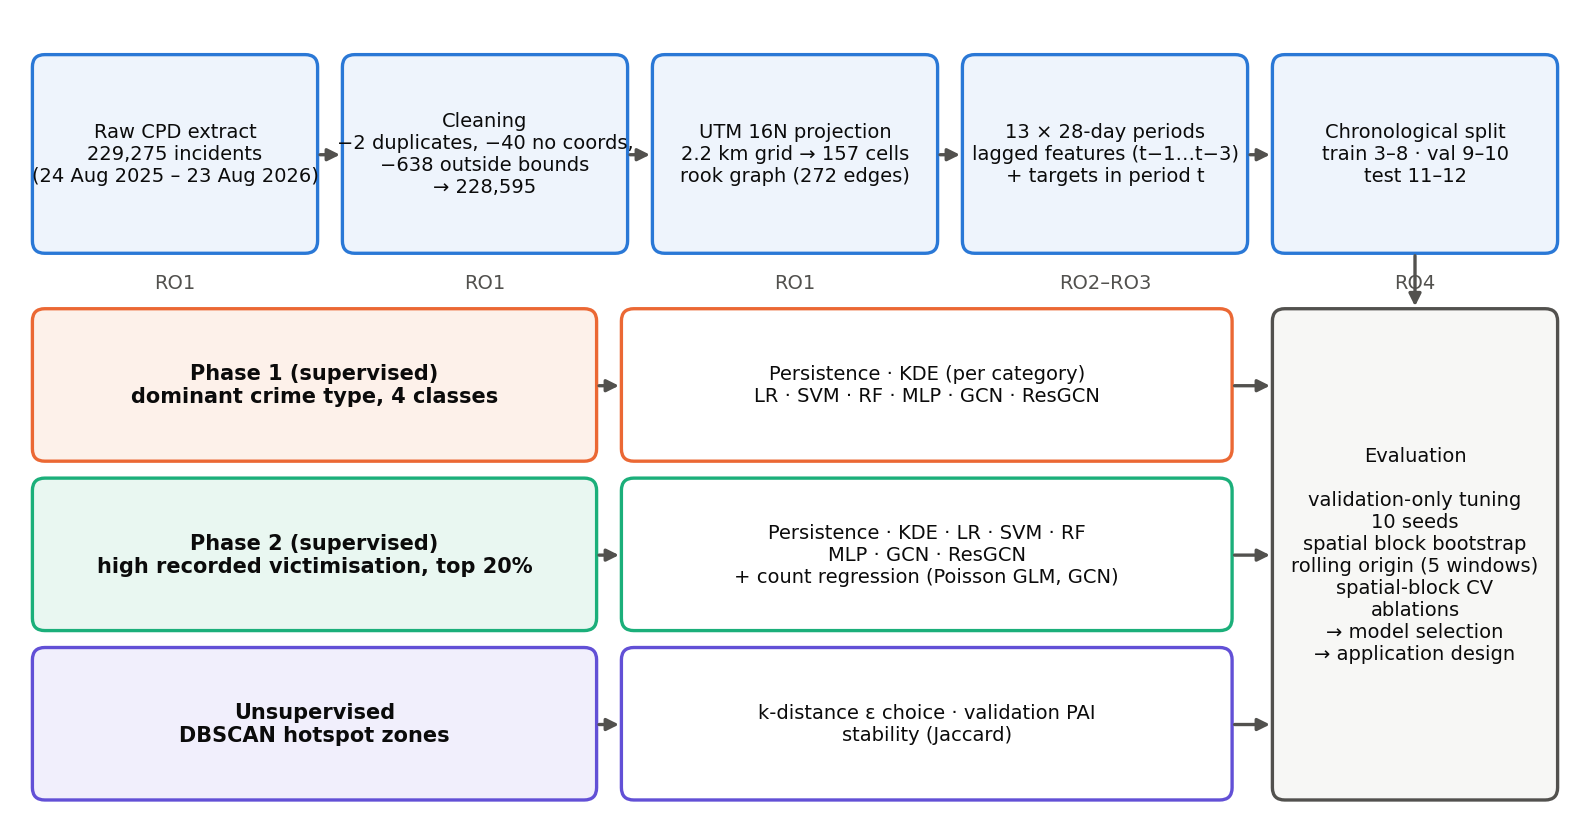
\includegraphics[width=\textwidth]{F01_pipeline.png}
\caption{Reproducible pipeline and mapping of stages to research objectives. All models in a phase share labels, features, splits and tuning budget.}
\label{fig:pipeline}
\end{figure}

\begin{figure}[H]
\centering
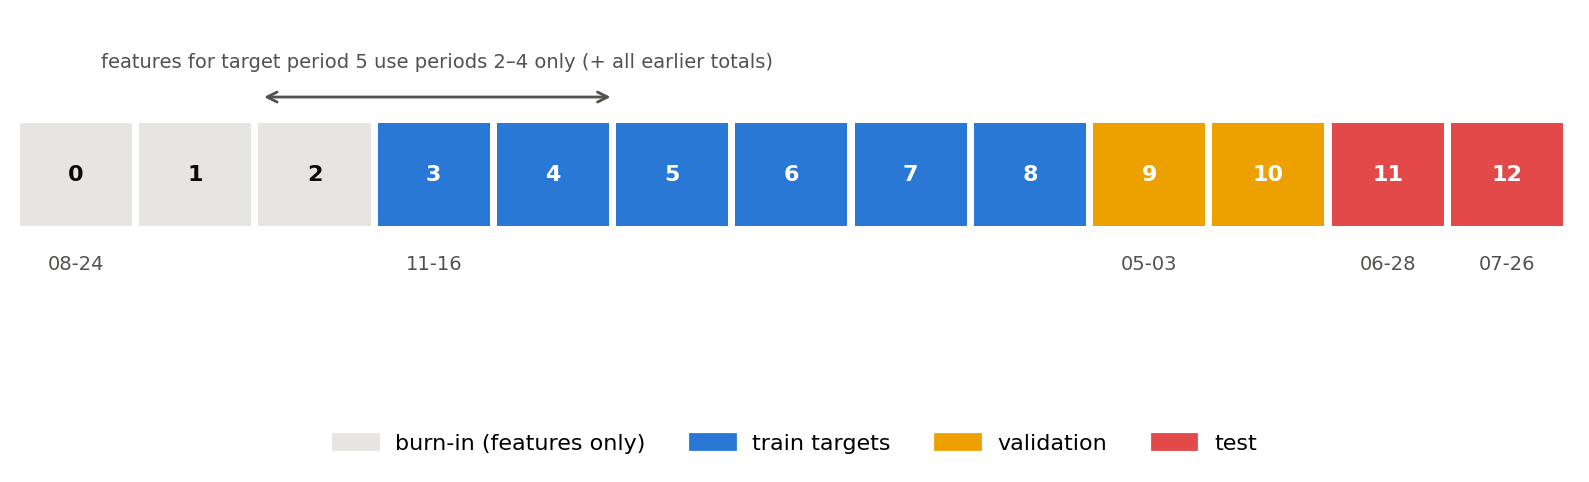
\includegraphics[width=0.95\textwidth]{F02_temporal_design.png}
\caption{Chronological design. Periods 0--2 provide only lagged features; the dates shown are the first days of selected periods.}
\label{fig:periods}
\end{figure}

Table~\ref{tab:romap} links each research objective to its method and supporting evidence.

\begin{table}[H]
\centering\small
\caption{Objective-to-method mapping}
\label{tab:romap}
\begin{tabularx}{\textwidth}{@{}L{2.6cm} Y L{3.6cm}@{}}
\toprule
Objective & Method & Evidence\\
\midrule
RO1 pipeline & Stage-by-stage cleaning log; UTM projection; grid; radius graph; history-only feature construction & Table~\ref{tab:clean}; Fig.~\ref{fig:graph}; E0, E13\\
RO2 crime type & Persistence, per-category KDE, LR, SVM, RF, MLP, GCN, ResGCN on four classes & E3, E5, E6, E8, E10\\
RO3 victimisation & Same model set with count regression; top 20\% decision rule & E1--E2, E4--E11\\
RO4 robustness & 10 seeds; spatial-block bootstrap; rolling origin; spatial-block CV; sensitivity & E7--E10\\
RO5 application & DBSCAN hotspot layer; PAI; runtime; architecture and governance design & E12--E14; \S\ref{sec:app}\\
\bottomrule
\end{tabularx}
\end{table}

\section{Data Collection and Preprocessing}
\label{sec:data}
\paragraph{Provenance.} The data include the CPD \emph{Crimes -- One year prior to present} extract from the City of Chicago Data Portal \citep{cpd2026}, obtained on 31 August 2026 as \path{Crimes_-_One_year_prior_to_present_20260831.csv} (17 fields; 229,275 rows; 24 August 2025 05:03 to 23 August 2026 00:00). Assessment~1 references the corresponding \emph{Crimes -- 2001 to Present} data set, but the filename and field names (such as \texttt{CASE\#}, \texttt{FBI CD}, and \texttt{DATE OF OCCURRENCE}) prove that the rolling one-year extract was used, hence the citation has been corrected. The website claims that the data is preliminary, can be reclassified, excludes the last seven days, and is released at block level for confidentiality reasons; all these factors transfer to the limitations (Section~\ref{sec:limits}). The data is a non-federal open dataset whose portal licence field reads ``See Terms of Use''; the City's terms supply the data ``as is'' without warranty, allow the City to require use to stop, and require any application built on it to state that the data have been modified from their original source \citep{chicago2026terms}, so the prototype dashboard carries that notice; the files do not include names or narratives but only block-level addresses and coordinates, used here for non-commercial research purposes only. The raw schema and the fields and missingness thereof can be seen in Appendix~\ref{app:dict} (Table~\ref{tab:schema}). In the three-year replication (Section~\ref{sec:multi}), the 509,905 records of the same portal's \emph{Crimes -- 2001 to Present} database \citep{cpd2026b} from 24~August~2023 to 23~August~2025 were collected on 25~October~2026 using the portal's API (17 fields, 106~MB, \path{Crimes_2001_to_present_subset_20230824_20250823.csv}) and appended to the one-year extract after harmonising field names and arrest and domestic flags.


\subsection{Data Cleaning}
\begin{table}[H]
\centering\small
\caption{Reconciled cleaning counts (E0)}
\label{tab:clean}
\begin{tabularx}{\textwidth}{@{}L{4.6cm} Y r r@{}}
\toprule
Stage & Rule & Remaining & Removed\\
\midrule
Raw records & All rows read; all 229,275 timestamps parsed & 229,275 & --\\
Exact duplicates & Identical across all 17 fields & 229,273 & 2\\
Missing coordinates & Latitude/longitude missing (the same 40 rows lack X/Y) & 229,233 & 40\\
Study boundary & Latitude 41.6--42.1; longitude $-87.9$ to $-87.5$ & 228,595 & 638\\
\bottomrule
\end{tabularx}
\end{table}
Assessment~1 identified 2 duplicates and 638 boundary exclusions but did not include the 40 records without coordinates, which is why their counts did not add up ($229{,}275-2-638=228{,}635\neq228{,}595$). Table~\ref{tab:clean} closes this discrepancy exactly. At this point, all missingness was limited to \texttt{LOCATION DESCRIPTION} (1,037 records, 0.45\%), set to \textsc{unknown} and only needed for counting distinct location types, and one missing \texttt{WARD}, which is unnecessary. There were 22 duplicate values of \texttt{CASE\#}, which are kept since one case may lead to multiple offenses. High-frequency cells were not considered outliers, as it was concentration that was modelled. The audit also revealed that the saved Phase~2 file by the pilot contained \texttt{HIST\_DOMESTIC} and \texttt{HIST\_ARREST} as concatenated ``Y/N'' values because the text flags were concatenated as strings instead of summed numerically, while the final pipeline sums the flags after converting them to 0/1 values.


\subsection{Data Transformation \& Feature Engineering}
\label{sec:transform}
\paragraph{Projection and grid.} Coordinates were transformed from WGS84 (EPSG:4326) to UTM zone~16N (EPSG:26916) such that distances are measured in metres. The grid origin is the minimum projected easting and northing of the cleaned data (425,477~m E; 4,610,479~m N), while the cell size is 2,200~m, thus matching the number of cells used by the pilot study, namely 157. Nodes are those cells that are occupied, with each having between 1 and 9,549 incidents (median 1,080). Seventeen cells, which are mostly located near the city borders or lakeshore, have fewer than 50 incidents per year; however, they were retained because their exclusion would bias the ranking towards the centre. Out of 1,570 modelled cell-periods, 68 showed no recorded event in the cell: this is a true zero in the victimisation task but has no dominant type, so it is excluded from the Phase~1 loss and statistics, while remaining a node in the graph.


\paragraph{Graph.} Cells whose centres are within 3~km are linked using a KD-tree radius query, resulting in 272 undirected (544 directed) edges, no self-loops stored and no isolated nodes. Since the cells form a regular lattice, the length of each edge is equal to 2.2~km: the diagonal neighbours have a distance of $2.2\sqrt{2}=3.11$~km and are out of the radius. The graph is thus a rook-adjacency lattice (degrees 1--4, average 3.46; Figure~\ref{fig:graph}), and the weights of the inverse-distance in the proposal are constant $1/2.2=0.455$, which GCN normalisation largely cancels. The pilot GCN also did not pass the edge weights to \texttt{GCNConv}. Both of these are examined in the graph ablation (E5), which includes graphs at queen (3.2~km), 4.5~km, and 6.6~km. A centroid-based variant, where edge lengths vary (0.68--3.0~km) and inverse distance weights contain information, was also examined (E19, Section~\ref{sec:posthoc}).

\begin{figure}[H]
\centering
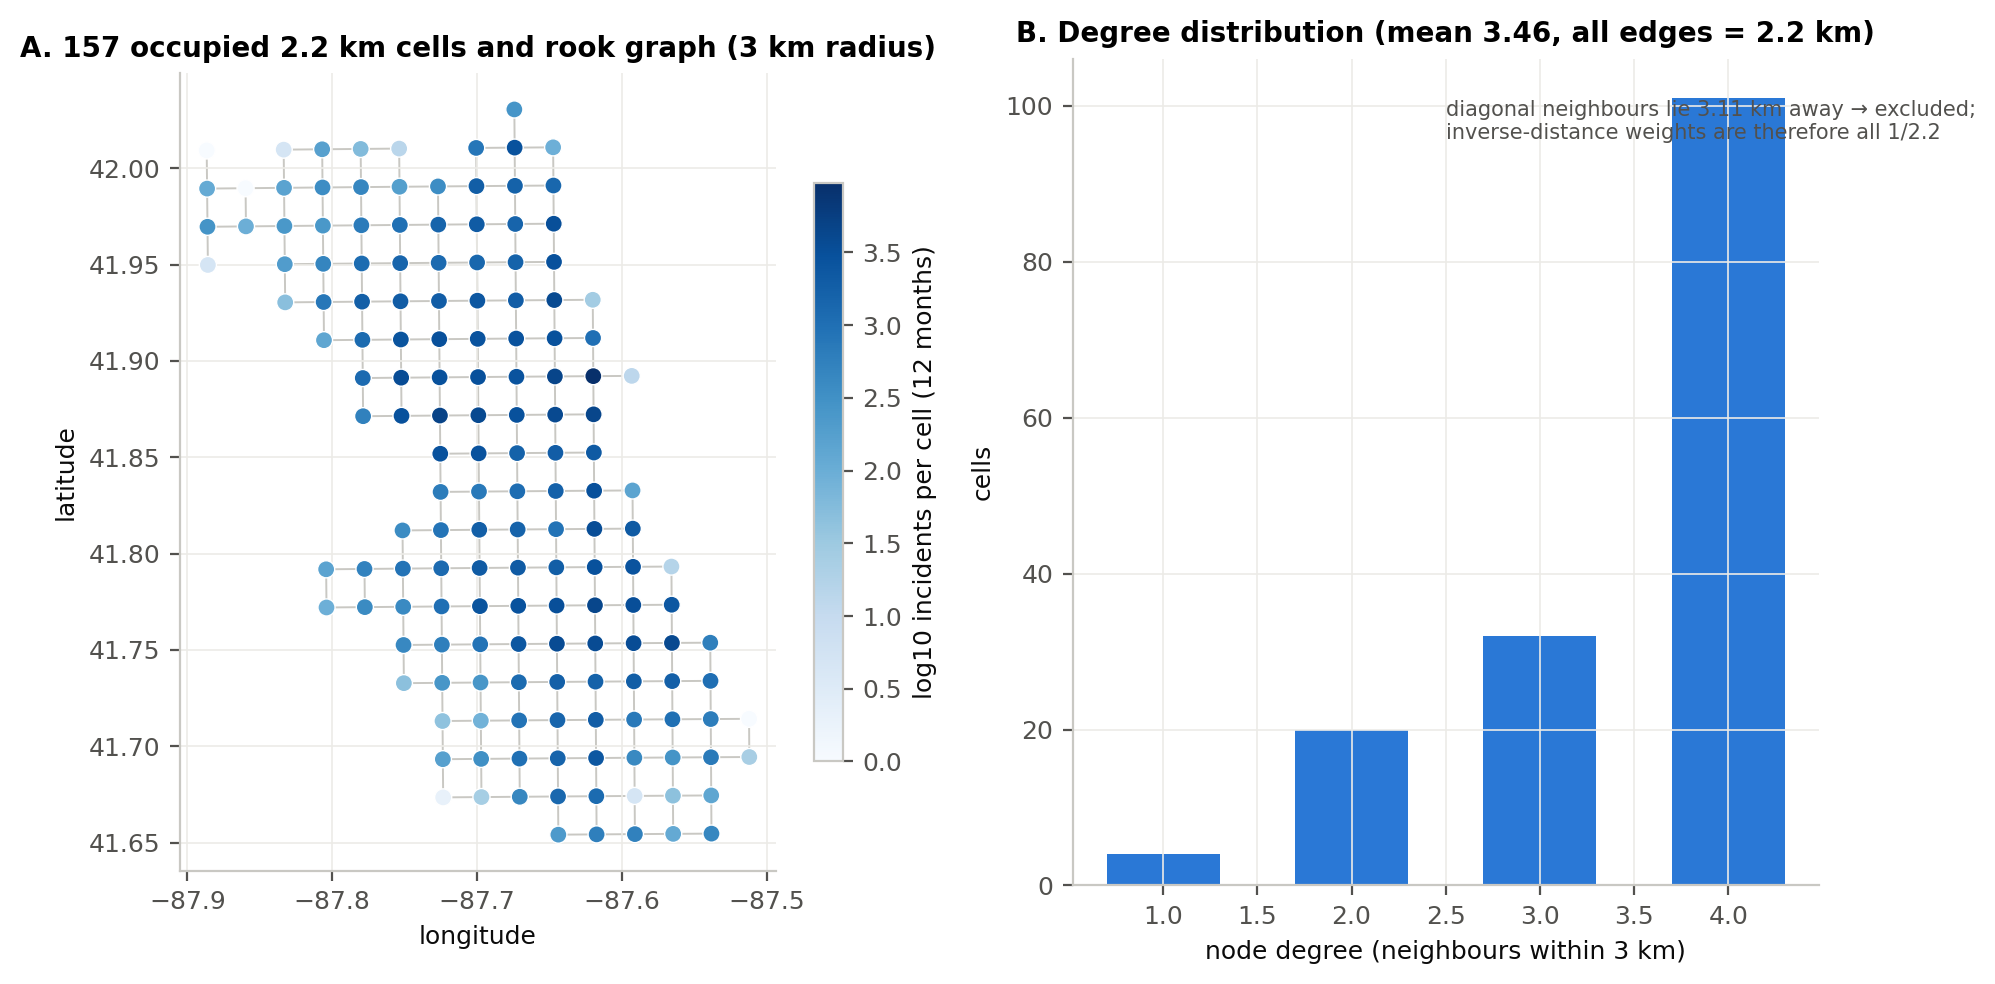
\includegraphics[width=\textwidth]{F04_grid_graph.png}
\caption{Occupied cells and the 3~km graph. Panel~B shows why inverse-distance weights carry no information on this lattice.}
\label{fig:graph}
\end{figure}

\paragraph{Targets.} In Phase~2, \texttt{Y\_VICTIM} is the number of person incidents in the cell in period $t$ (73,494 records, 32.2\% of the cleaned data; the reasons for category selection are provided in Appendix~\ref{app:dict}). A cell is considered \emph{high} if it has an incident count equal to or greater than the 80th percentile in that period among the 157 cells. Ties at the cutoff result in prevalence between 20.4 and 22.3\% per period (32--35 cells). Percentiles are used only retrospectively to define labels; when predicting, the program ranks the cells and marks the best 32 (20\%). No future outcome is needed to make the prediction, and no held-out outcome is used to choose a threshold.

In Phase~1, categories with fewer than 1,000 instances were collapsed to \textsc{other} (Pilot Rule), the dominant category was calculated for each cell period (ties resolved in favour of the more frequent one), and those categories that were dominant in at least 5\% of \emph{training} cell periods were selected as classes. The training data only retained \textsc{theft} (42.5\%), \textsc{battery} (38.8\%), and \textsc{criminal damage} (7.0\%) classes; all other categories were dominant in no more than 2.6\% of cell periods and were collapsed to \textsc{other\_type}. The collapsing eliminates the singleton class (one \textsc{sex offense} cell) that prevented stratified folds in the Pilot case.

\paragraph{Features.} A total of twenty-three features were created for each cell/target combination for earlier periods only (Appendix~\ref{app:dict}, Table~\ref{tab:dict}). These include victimisation counts and total counts at lags 1 to 3, long-run means of all previous periods, the victimisation, domestic, arrest and night-time shares of all previous incidents, crime mix of three periods (share of eight common types), trend for one to three periods (lag~1 minus lag~3), and coordinates of the cell centre. Counts were log-transformed with $\log(1+x)$, and the trend with the signed logarithm since counts have strong right-skewness (cell means span from 0 to over 150 per time period). All features were then standardised using the mean and standard deviation from only the training rows. Two neighbour average features were constructed using the row-normalised adjacency matrix only for the spatial lag ablation study.


\begin{figure}[H]
\centering
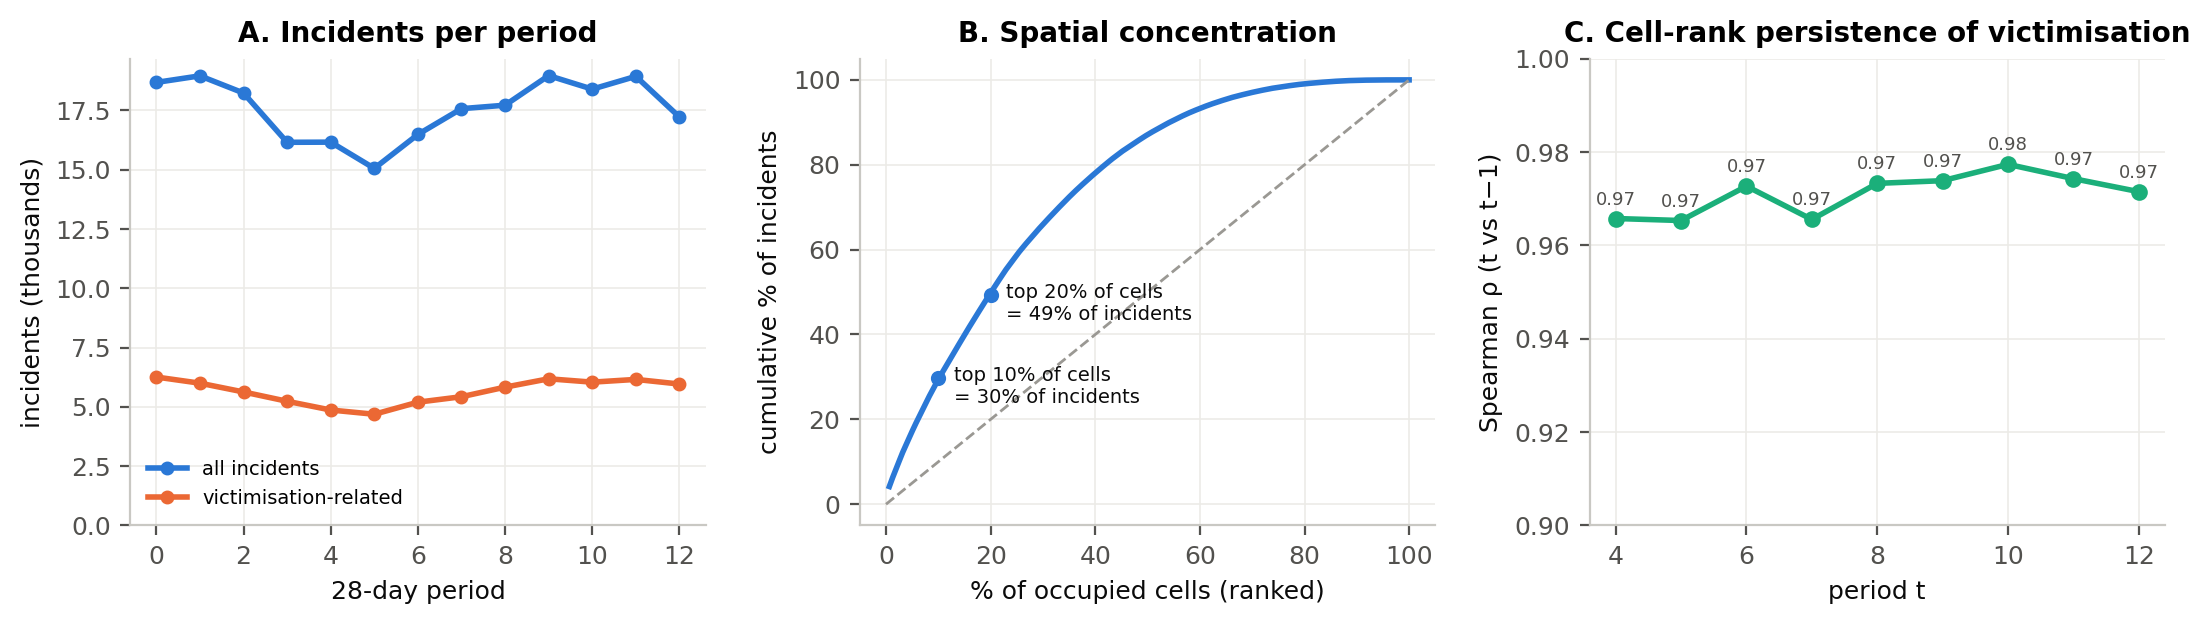
\includegraphics[width=\textwidth]{F03_eda.png}
\caption{Exploratory analysis: (A) incidents per period; (B) concentration of incidents across cells; (C) Spearman correlation between consecutive periods' cell victimisation counts.}
\label{fig:eda}
\end{figure}
Figure~\ref{fig:eda} highlights some insights gained from exploratory analysis that guided the design process. There is a dip in volumes during the winter periods (4-5) and an increase during the summer periods, hence the choice of a relative per period label based on the ranking as opposed to an absolute count threshold. Concentration (Panel~B) supports aggregation at the area level. Most importantly, Panel~C reveals that ranking cells in terms of victimisation does not change much between periods (Spearman $\rho =0.965$-$0.977$), so rankings are more stable than raw counts, which predicts that persistence will be a very strong baseline.

\subsection{Class Imbalance Resolution}
The Phase~2 dataset has a 1:4 imbalance by construction. Three approaches were compared using identical splits (E4): no correction, inverse-frequency class weights, and SMOTE \citep{chawla2002,lemaitre2017} applied only to the training rows of the tabular LR model. Each approach was evaluated at a 0.5 threshold and at a threshold selected using validation data. SMOTE was not applied to graph-based models because synthetic nodes would require invented edges and coordinates without spatial meaning. Instead, class-weighted cross-entropy (Equation~\ref{eq:loss}) was used for the GCN, ResGCN and MLP. The main decision rule---flagging the 32 highest-ranked cells in each period---matches the prevalence by construction and is unaffected by probability calibration. For Phase~1 (test class shares of 45/9/37/10\%), all models used balanced class weights, and macro-F1 served as the selection metric, giving every class equal importance, including the less common \textsc{criminal damage} and \textsc{other\_type} classes


\subsection{Feature Selection}
No automatic feature selection was employed. Given 23 features and 942 training cell-periods, L2 regularisation in LR and weight decay in neural models stabilize variance better than feature selection, which itself requires validation data. Feature group ablations (E6) evaluate if victimisation history, crime mix proportions, and coordinates are required, as well as whether removing composition features changes Phase~1, given that same-period composition features had caused leakage in the pilot.

\subsection{Dimensionality Reduction}
Dimensionality reduction was not considered necessary. The space of the features is low-dimensional, the features are meaningful and partially correlated by design (victimisation counts form a part of the total counts), and the use of principal components would destroy the interpretability that is required for the explanation module of the application. Collinearity is addressed using regularisation and is acknowledged when interpreting coefficients.

\subsection{Feature Importance Assessment}
\label{sec:importance}
Importance was computed only on the validation data (E14), replacing the planned SHAP analysis in Assessment~1, as, for a linear model, coefficients and permutation importance provide an adequate explanation. The six largest LR coefficients are listed in Table~\ref{tab:imp}.

\begin{table}[H]
\centering\small
\caption{Phase~2 feature importance on validation periods 9--10 (E14)}
\label{tab:imp}
\resizebox{\textwidth}{!}{\begin{tabular}{@{}lrrr@{}}
\toprule
Feature & LR standardised coefficient & LR permutation $\Delta$AP & RF permutation $\Delta$AP ($\pm$ sd)\\
\midrule
Mean victimisation, all previous periods & $+5.64$ & 0.267 & $0.057\pm0.027$\\
Total incidents, lag 1 & $+4.16$ & 0.142 & $0.007\pm0.011$\\
Mean total incidents, all previous periods & $+3.99$ & 0.129 & $0.007\pm0.011$\\
Victimisation share of all previous incidents & $+3.99$ & 0.214 & $0.007\pm0.005$\\
Assault share, last 3 periods & $-2.68$ & 0.035 & $-0.001\pm0.003$\\
Battery share, last 3 periods & $-2.31$ & 0.030 & $0.006\pm0.005$\\
\bottomrule
\end{tabular}}
\end{table}
Long-run victimisation mean is the top variable in both models: shuffling it decreases validation AP by 0.27 for LR. Then come recent total volume and historical victimisation share. The negative coefficients on the assault and battery shares depend on the victimisation mean already in the model and thus should not be interpreted causally. RF distributes feature importance among correlated counts, so its individual decrease is modest. This ranking guided the choice of features in the explanation panel for the application (Section~\ref{sec:app}) and the ``victimisation lags only'' ablation (E6).

\section{Machine Learning Models}
Models were selected to distinguish four types of skill: persistence, spatial averaging, flexible table-based learning, and graph learning. The GCN and non-graph MLP have the same depth, width options and training code, so that any difference in their behaviour reflects the effect of message passing. All used models are listed in Table~\ref{tab:models} together with hyperparameters optimised on the validation dataset.

\begin{table}[H]
\centering\scriptsize
\caption{Implemented models and validation-selected hyperparameters (P1 = Phase~1, P2 = Phase~2)}
\label{tab:models}
\begin{tabularx}{\textwidth}{@{}L{2.0cm} Y L{4.6cm} L{2.4cm}@{}}
\toprule
Model & Specification & Selected hyperparameters & Role\\
\midrule
Majority & Predict majority class; AP equals prevalence & -- & Null reference\\
Persistence & P2 score $=1\cdot L_1+0.5\cdot L_2+0.25\cdot L_3$ (recency-weighted victimisation lags); P1 dominant category of last three periods & -- & Concentration theory\\
KDE & Gaussian KDE of incidents in previous three periods, evaluated at cell centres; P1 uses one count-scaled KDE per category, argmax & Bandwidth 800~m (P1 and P2) & Traditional hotspot method\\
LR & L2-regularised logistic / multinomial regression, balanced class weights & $C=10$ (P2); $C=100$ (P1) & Interpretable baseline\\
SVM (RBF) & Kernel SVM, balanced weights; decision function used for ranking & $C=10,\gamma=0.01$ (P2); $C=0.1$, $\gamma$=scale (P1) & Proposal baseline\\
Random forest & 300 trees, balanced-subsample weights \citep{breiman2001} & Unlimited depth, leaf 1 (P2); leaf 5 (P1) & Non-linear tabular baseline\\
MLP & Two linear layers, ReLU, dropout; same code path as GCN without edges & $h=128,p=0.3,\eta=0.01,\lambda=5\times10^{-3}$ (P2); $h=32,p=0.3,\eta=0.003$ (P1) & Graph ablation\\
GCN & Two \texttt{GCNConv} layers with self-loops, symmetric normalisation and edge weights \citep{kipf2017} & $h=64,p=0.3,\eta=0.01,\lambda=5\times10^{-4}$ (P2); $h=64,p=0.5,\lambda=5\times10^{-3}$ (P1) & Proposal primary model\\
GAT & Two \texttt{GATConv} layers, 4 attention heads, ELU; learned neighbour weights, edge weights unused \citep{velickovic2018} & $h=64,p=0.3,\eta=0.01,\lambda=5\times10^{-4}$ (P2); $h=128$ (P1) & Learned-neighbourhood test\\
ResGCN & GCN layer plus separate linear self path in each layer (Equation~\ref{eq:resgcn}) & $h=128,p=0.3,\eta=0.003,\lambda=5\times10^{-3}$ (P2); $h=64,p=0.3$ (P1) & Optimisation from smoothing analysis\\
DBSCAN & Density clustering of victimisation incident coordinates \citep{ester1996} & $\varepsilon=300$~m, minPts $=60$ & Unsupervised hotspot layer\\
Poisson GLM; GCN-Poisson & Next-period count regression with log link & GLM $\alpha=1$ & Continuous score (E11)\\
\bottomrule
\end{tabularx}
\end{table}

\paragraph{GCN propagation.} With weighted adjacency $A$, self-loops $\tilde{A}=A+I$ and degree matrix $\tilde{D}$, one layer computes
\begin{equation}
H^{(l+1)}=\sigma\!\left(\tilde{D}^{-1/2}\tilde{A}\tilde{D}^{-1/2}H^{(l)}W^{(l)}\right).
\label{eq:gcn}
\end{equation}
For node $i$ with degree $d_i$ on an equally weighted graph, the weight on its own features is $1/(d_i+1)$ and on neighbour $j$ it is $1/\sqrt{(d_i+1)(d_j+1)}$. For this rook lattice (average degree 3.46), the weight on its own history for a typical cell is therefore only about 0.2 after one layer, and even less after two. With the inverse-distance weights being constant, scaling of the matrix $A$ by $1/2.2$ affects only the self-weight through the self loop, which explains why the weighted and unweighted graphs behave almost identically (E5). For a target where the rank is that of the \emph{own} cell, this process blends a highly victimised cell with its less victimised neighbouring cells. This analysis led to two decisions, made before test evaluation and based on validation results: to investigate the depth and graph radius, and to include a residual self path,
\begin{equation}
H^{(l+1)}=\sigma\!\left(\hat{A}H^{(l)}W_n^{(l)}+H^{(l)}W_s^{(l)}\right),\qquad \hat{A}=\tilde{D}^{-1/2}\tilde{A}\tilde{D}^{-1/2},
\label{eq:resgcn}
\end{equation}
so that the model is able to learn how much neighbour data it needs instead of having this determined through node degree. The model resembles the self/neighbour separation of GraphSAGE-style architectures and was implemented using PyTorch and PyTorch Geometric \citep{paszke2019,fey2019}.

\paragraph{Loss and regularisation.} Classification networks minimise class-weighted cross-entropy over labelled nodes $V_L$,
\begin{equation}
\mathcal{L}=-\frac{1}{|V_L|}\sum_{i\in V_L}w_{y_i}\log\hat{p}_{i,y_i},\qquad w_c=\frac{n}{K\,n_c},
\label{eq:loss}
\end{equation}
where $n_c$ represents the number of training nodes belonging to class $c$ out of $K$ classes. The weight increases the gradient contribution for minority classes, which is cost-sensitive learning due to imbalance \citep{he2009}. Adam with weight decay $\lambda$ applies L2 regularisation by adding $\lambda\lVert W\rVert^2$, which is important because there are 157 nodes per snapshot.

\paragraph{Logistic regression and SVM.} LR models the log-odds as linear in the standardised features and minimises
\begin{equation}
\min_{\beta}\;\tfrac{1}{2}\lVert\beta\rVert^2+C\sum_i w_{y_i}\log\!\left(1+e^{-\tilde{y}_i\beta^\top\mathbf{x}_i}\right),\qquad P(y=1\mid\mathbf{x})=\frac{1}{1+e^{-\beta^\top\mathbf{x}}},
\label{eq:lr}
\end{equation}
with \(\tilde{y}_i\in\{-1,1\}\), so higher \(C\) implies weaker regularisation. The validation search selected \(C=10\) for the model using 23 standardised predictors. Validation AP ranged from 0.964 to 0.968 across the tested values of \(C\), indicating that performance was relatively insensitive to this choice and that the 23 standardised features are not over-fitted at this sample size. The RBF-SVM maximises the margin in the feature space defined by \(k(\mathbf{x},\mathbf{x}')=\exp(-\gamma\lVert\mathbf{x}-\mathbf{x}'\rVert^2)\) \citep{cortes1995}; the small \(\gamma=0.01\) selected for Phase~2 produces a smooth decision boundary, described here as nearly linear and consistent with the LR result.



\paragraph{KDE.} Density in the cell centre $s$ from $n$ incidents $s_j$ occurring in the past three periods is
\begin{equation}
\hat{f}(s)=\frac{1}{2\pi n h^{2}}\sum_{j=1}^{n}\exp\!\left(-\frac{\lVert s-s_j\rVert^{2}}{2h^{2}}\right).
\label{eq:kde}
\end{equation}
Bandwidth $h$ controls the trade-off between bias and variance \citep{silverman1986}. Validation AP peaked at 0.936 when $h=800$~m  but decreased to 0.774 at $h=3,000$~m. The wider kernels blurred neighbouring high- and low-victimisation cells, producing the same over-smoothing problem observed in the GCN.

\section{Model Training Process}
\paragraph{Splits.} Unit of observation is a cell-period. Training data uses $6\times157=942$ rows for Phase~2 (919 non-zero rows for Phase~1), validation uses 314, and the test set uses 314 (Phase~2) and 303 (Phase~1). The observations are not independent: the same 157 cells appear repeatedly and neighbours are correlated, thus the sample size is much less than the number of incidents (228,595) and is closer to the number of cells. Chronological splitting has been selected over random node splitting in order to ensure that each test prediction is an actual forecast; the two-period test window gives 314 test rows compared to 24 cells in the pilot.

\paragraph{Graph protocol.} Each period constitutes a separate snapshot of the same graph, and the snapshots are combined into a block-diagonal graph so that messages do not pass between periods. The protocol is \emph{inductive in time}: all node features, derived only from historical information, and all edges are available at inference, while no labels from the target period are used. In the spatial-block experiment (E9), the protocol is \emph{transductive in space}: held-out cells remain in the graph with their historical features, but their labels are excluded from the loss calculation and early stopping.


\paragraph{Optimisation and convergence.} Neural models were trained using full-batch Adam for up to 400 epochs, with early stopping (patience 60) based on validation AP (Phase~2) or macro-F1 (Phase~1), restoring the best checkpoint. Tabular models were fitted using scikit-learn \citep{pedregosa2011}. Training is fast: a GCN converges in approximately 0.45~s and LR in approximately 4~ms on the CPU (Table~\ref{tab:cost}). Figure~\ref{fig:curves} shows that the GCN's validation AP increases rapidly before levelling off below the MLP's, suggesting architectural bias rather than insufficient training.

\begin{figure}[H]
\centering
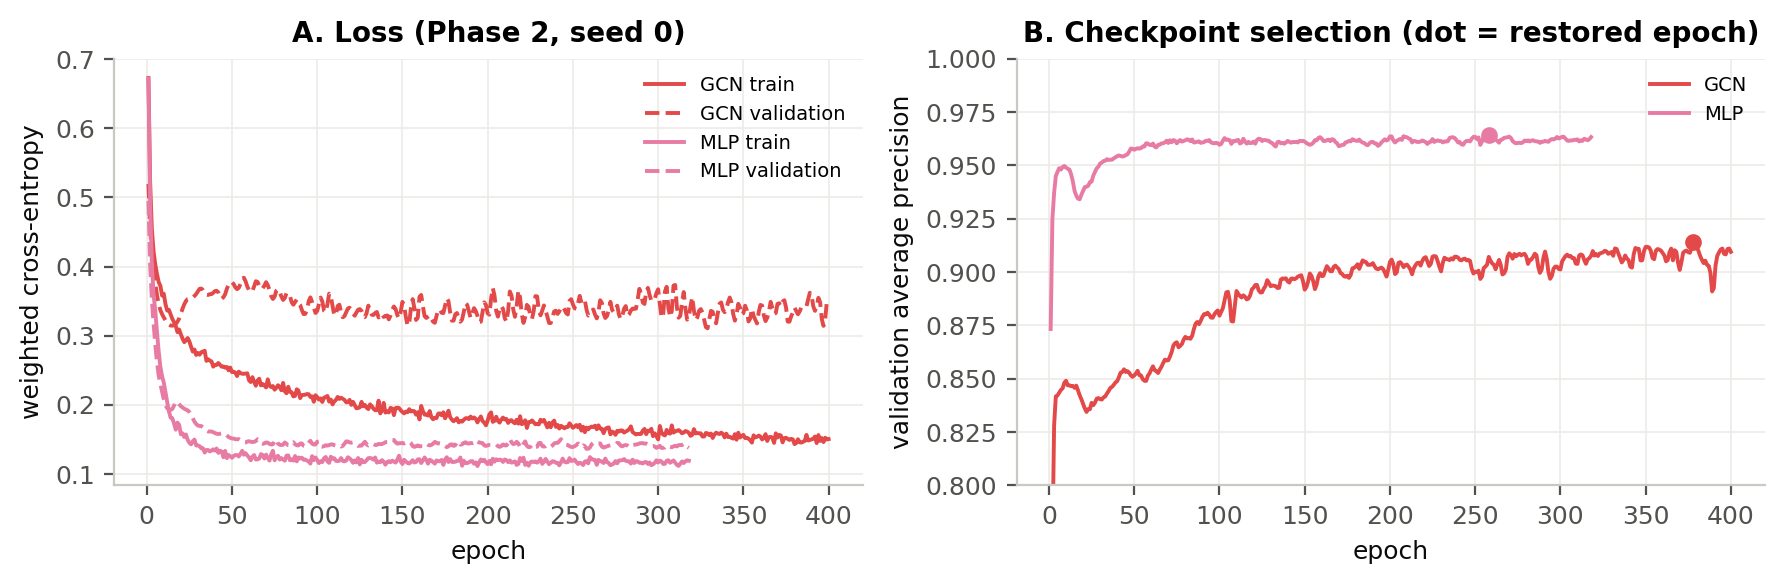
\includegraphics[width=0.85\textwidth]{F08_training_curves.png}
\caption{Phase~2 training curves (seed 0). Both models converge; the GCN plateaus at a lower validation AP than the MLP.}
\label{fig:curves}
\end{figure}

\paragraph{Reproducibility.} Software: Python 3.9.6, NumPy 2.0.2, pandas 2.3.3, scikit-learn 1.6.1, PyTorch 2.8.0, PyTorch Geometric 2.6.1, pyproj 3.6.1 and imbalanced-learn 0.12.4 on macOS (Apple M5, 10-core, 16~GB RAM). All stochastic models used seeds 0--9. As the split is determined exclusively by the dates (Appendix~\ref{app:split}, Table~\ref{tab:periods}), no random-split manifest is needed. The entire suite of experiments takes less than ten minutes of compute time with maximum memory usage of 0.94~GB.

\section{Validation}
\paragraph{Hyperparameter optimisation.} In Assessment~1, the base paper's hyperparameters were followed, but with a promise of further optimisation to come. This was reconciled with a validation-only approach: each model had a grid search performed over periods 9--10, neural networks were optimised over three seeds, and the test periods were only used once, after all decisions were made. The grid searches consisted of the following: LR $C\in\{0.01,0.1,1,10,100\}$; SVM $C\in\{0.1,1,10,100\}\times\gamma\in\{\text{scale},0.01,0.1\}$; RF depth $\in\{3,6,\text{none}\}\times$ minimum leaf $\in\{1,5\}$; MLP/GCN/ResGCN hidden $\in\{32,64,128\}\times$ dropout $\in\{0.3,0.5\}\times$ learning rate $\in\{0.01,0.003\}\times$ weight decay $\in\{5\times10^{-4},5\times10^{-3}\}$ (24 configurations $\times$ 3 seeds); KDE bandwidth $\in\{300,500,800,1200,2000,3000\}$~m. The depth and graph radius were then tested as ablations (E5) and were \emph{not} used for selecting the reported models. Model selection was performed according to the stated rule: the best validation performance in each phase, where the simpler model was selected only if the performances differed by less than one seed standard deviation. The Assessment~1 suggested a smaller grid (learning rate $\{0.001,0.01\}$, hidden width $\{64,128\}$, dropout $\{0.3,0.5\}$); the final grid includes these widths and dropouts, uses learning rates $\{0.01,0.003\}$ (0.001 was not considered), and incorporates weight decay and widths of 32 for the neural models, hence it is a superset, except for the learning rate.


\paragraph{Over- and under-fitting.} The highest validation AP achieved by the GCN (0.910) was lower than that of any tabular method and the MLP (0.962--0.968), with low seed variation (sd $\leq0.004$). Therefore, the gap is architectural, not caused by overfitting; having more neurons or reducing the dropout ratio did not narrow the gap. The pilot GCN configuration (128 units) was not chosen for either phase. Weight decay with a value of $5\times10^{-3}$ was favoured by both the MLP and ResGCN models consistent with the small training graph.

\paragraph{Robustness designs.} Four additional designs address different generalisation questions: (i)~ten training seeds assess randomness in the optimisation process; (ii)~a \emph{rolling origin} (E8) retrains on all preceding periods before each test period 8--12, assessing stability over time; (iii)~\emph{spatial-block cross-validation} (E9) holds out five k-means blocks of cells to assess transfer to unseen areas; and (iv)~a \emph{spatial-block bootstrap} (E10) resamples 26 blocks of \(3\times3\) cells (6.6~km squares) with replacement 2,000 times, keeping both test periods of each block together, to obtain confidence intervals and paired model differences that account for spatial dependence \citep{roberts2017}. Stratified five-fold cross-validation of cells, proposed in Assessment~1, was not used because it would mix periods (temporal leakage) and because the rare Phase~1 classes cannot appear in every fold. Nested cross-validation was considered unnecessary because the validation-then-test procedure already separates model tuning from evaluation. However, the selected configurations may have optimistic validation scores, so conclusions are based only on test scores.



Table~\ref{tab:evtypes} summarises the evaluation designs and the generalisation question each answers.

\begin{table}[H]
\centering\scriptsize
\caption{Evaluation designs and the generalisation question each answers}
\label{tab:evtypes}
\begin{tabularx}{\textwidth}{@{}L{3.2cm} Y L{3.4cm}@{}}
\toprule
Design & Question answered & Used here\\
\midrule
Random node split & Can the model interpolate between cells it has seen? (optimistic when cells and periods are correlated) & Assessment~1 pilot only; replaced\\
Chronological hold-out & Can it forecast a future period from the past? & E1--E3 (periods 11--12); E21 (33--38)\\
Rolling origin & Is forecasting skill stable as the origin moves, and across seasons? & E8 (5 windows); E21 (12 windows)\\
Spatial-block hold-out & Can it transfer to areas whose labels it never saw? & E9 (5 k-means blocks, labels masked)\\
Spatial-block bootstrap / permutation & How uncertain are differences given spatial dependence? & E10, E16 ($3\times3$-cell blocks)\\
\bottomrule
\end{tabularx}
\end{table}


\section{Evaluation}
Phase~2 is a ranking task with 21\% prevalence. The main metric is \textbf{average precision (AP)}, the step-wise area under the precision--recall curve calculated using scikit-learn (not trapezoidal PR-AUC), which reflects minority-class performance \citep{saito2015}. The decisions are measured with the practical \textbf{top-20\% rule} (select 32 cells per period), measuring positive-class F1 and macro-F1 (the average of the high-class and low-class F1; this is the metric used in the RO3 criterion). Metrics at a validation-tuned probability threshold, ROC-AUC and the Brier score are secondary. For Phase~1, the main metric is macro-F1 for the four classes, with accuracy, weighted F1, balanced accuracy, Cohen's $\kappa$ and per-class F1. Following \citet{sokolova2009},
\begin{gather}
\mathrm{Precision}=\frac{TP}{TP+FP},\quad \mathrm{Recall}=\frac{TP}{TP+FN},\quad F_1=\frac{2PR}{P+R},\quad \mathrm{Accuracy}=\frac{TP+TN}{N},\label{eq:prf}\\
\text{macro-}F_1=\frac{1}{K}\sum_{c=1}^{K}F_{1,c},\qquad \text{weighted-}F_1=\sum_{c=1}^{K}\frac{n_c}{N}F_{1,c},\qquad \mathrm{AP}=\sum_k (R_k-R_{k-1})P_k,\label{eq:macro}\\
\mathrm{Brier}=\frac{1}{N}\sum_{i}(\hat{p}_i-y_i)^2,\qquad \mathrm{PAI}=\frac{n_{\mathrm{hot}}/n}{a_{\mathrm{hot}}/a}.\label{eq:brier}
\end{gather}
ROC-AUC is the probability that a randomly selected high cell is ranked above a randomly selected low cell. The null references are different for each measure: the AP for a random ranking is the prevalence (0.21), the macro-F1 of the all-low classifier is 0.44, and Phase~1 majority accuracy is 0.37 with macro-F1 0.13. Thus, 0.5 is not a universal chance line. For the hotspot perspective, the PAI \citep{chainey2008} is the ratio of the percentage of victimisation events from the test period to the percentage of cells selected. For count regression (E11), a truly continuous problem, MAE, RMSE, $R^2$ and Spearman $\rho$ are used.

\section{Chapter Summary}
The methodology transforms the pilot's random and partially circular design into a chronological and history-only forecasting design; aligns labels, features, and tuning budgets for nine model families; settles the hyperparameter dilemma with a validation-only search; and gauges uncertainty with blocked designs. The mathematics of graph normalisation and kernel bandwidth influenced two specific design decisions---the residual GCN and the graph and bandwidth searches---whose impact is evaluated in the next chapter.

% =====================================================================
\chapter{Results and Discussion}
\label{ch:results}
This chapter first distinguishes the Assessment~1 pilot evidence from the new final experiments before presenting their results. These results are interpreted in relation to the research questions and objectives, followed by an analysis of limitations and challenges and a design for converting the work into an application. Unless specified otherwise, "test" refers to periods 11--12 (28~June to 22~August~2026), which were used only once after all choices had been finalised.

\section{Results}
\subsection{Experimental Design and Registry}
All experiments are presented in Table~\ref{tab:registry}. Experiments E0--E14 and E20--E21 adhere to the design determined before analysis of the test periods; experiments E15--E19 and E22--E24 are defined as \emph{post-hoc}, since they were designed after the main test results were obtained, to fill gaps revealed during the review of the report; thus any choice in them is based on validation data exclusively and cannot influence the chosen models from Sections~\ref{sec:p2res}--\ref{sec:p1res}. All experiments finished. Tuning budget (validation only): LR 5 values of $C$; SVM 12 settings; RF 6; KDE 6 bandwidths; and for each neural model (MLP, GCN, ResGCN, GAT) 24 configurations $\times$ 3 seeds; the final models used 10 seeds, while the ablation and sensitivity studies used 5. Each varies only one parameter from the primary baseline and uses the same splits, labels and tuning budget. "Seeds" refers to how many training seeds were tried on stochastic models.


\begin{table}[H]
\centering\scriptsize
\caption{Experiment registry (all experiments completed; outputs in \texttt{Assessment2/results})}
\label{tab:registry}
\begin{tabularx}{\textwidth}{@{}l L{3.4cm} Y L{2.3cm} L{1.6cm} l@{}}
\toprule
ID & Question & Design / changed factor & Models & Metric & Seeds\\
\midrule
E0 & Are pilot results valid? & Reconcile counts; leakage rule; reproduce pilot split with LR & Pilot GCN (reported), LR, persistence & Accuracy, macro-F1, AP & --\\
E1 & Best hyperparameters? & Validation-only grid search (periods 9--10) & All & Val.\ AP / macro-F1 & 3\\
E2 & P2 test comparison & Chronological test, periods 11--12 & 8 models + majority & AP, macro-F1, AUC, Brier & 10\\
E3 & P1 test comparison & Same design, four classes & 8 models + majority & Macro-F1, $\kappa$, per-class F1 & 10\\
E4 & Does imbalance handling help? & None / class weights / SMOTE; 0.5 vs tuned threshold & LR, GCN & Threshold F1, AP & 10\\
E5 & Does the graph help? & Radius, weighting, depth; spatial-lag features & GCN, ResGCN, LR & AP, macro-F1 & 10\\
E6 & Which features matter? Leakage? & Remove feature groups & LR, GCN & AP, macro-F1 & 5\\
E7 & Sensitive to label or grid? & 70/80/90th percentile; 1.5/2.2/3.0~km cells & Persistence, LR, GCN, ResGCN & AP, AUC & 5\\
E8 & Stable over time? & Rolling origin, test periods 8--12 & Persistence, KDE, LR, GCN, ResGCN & AP, macro-F1 & 5\\
E9 & Transfer to unseen areas? & Five spatial blocks held out (labels masked) & Persistence, LR, MLP, GCN, ResGCN & AP, AUC & 5\\
E10 & Signal or chance? & Spatial-block bootstrap (26 blocks, 2,000 reps); paired differences & All & AP, macro-F1 CIs & --\\
E11 & Can counts be forecast? & Continuous next-period count & Persistence, Poisson GLM, GCN, MLP & MAE, RMSE, $R^2$ & 5\\
E12 & Unsupervised hotspots useful? & DBSCAN grid; validation PAI; stability & DBSCAN vs ranked models & PAI, hit rate & --\\
E13 & Cost? & Fit/inference time, memory, parameters & All & Seconds, MB & --\\
E14 & Why does it predict? & Coefficients, permutation importance (validation) & LR, RF & $\Delta$AP & --\\
E15 & Does preprocessing help? (post-hoc) & Raw / z-score / log / log+z-score / robust scaling; drop low-volume cells & LR, MLP, GCN, ResGCN & AP, macro-F1 & 5\\
E16 & Are differences real? (post-hoc) & Paired spatial-block permutation tests, Holm-corrected & All & AP, macro-F1 & --\\
E17 & Can Phase 1 features improve? (post-hoc) & +18 history-only features, validation-selected & LR, RF, MLP, ResGCN & Macro-F1 & 5\\
E18 & Are count models fairly tuned? (post-hoc) & Tuned neural count models; $\alpha$ grid to 100 & GLM, MLP, GCN, ResGCN, GAT & MAE, RMSE, $R^2$ & 5\\
E19 & Effective sample size; weighted graph? (post-hoc) & Moran's $I$, lag-1 correlation; centroid-based graph & GCN, ResGCN, GAT & $n_\mathrm{eff}$, AP & 10\\
E20 & Does the prototype work? & 20 automated API tests, serving parity, latency & LR champion & Pass/fail, ms & --\\
E21 & Do findings hold over three years? & 24 train / 6 validation / 6 test periods; 12-window rolling origin & All & AP, macro-F1 & 10\\
E22 & Does a narrower victimisation label change the ranking? (post-hoc) & FBI index violent crime only; re-tuned on validation & Persistence, KDE, LR, RF, MLP, GCN, ResGCN & AP, macro-F1 & 5\\
E23 & Are errors spread evenly across poorer and richer areas? (post-hoc) & Test errors by community-area hardship tercile; cell bootstrap & LR, persistence, RF, MLP, GCN, ResGCN & Recall, FPR, flag rate, macro-F1 & --\\
E24 & Does gradient boosting add skill? (post-hoc) & Histogram gradient boosting, 8-setting validation grid & HGB & AP, macro-F1 & 5\\
\bottomrule
\end{tabularx}
\end{table}

\subsection{Pilot Audit: Reported versus Reproduced Evidence (E0)}
\label{sec:audit}
Table~\ref{tab:pilot} contrasts what was \emph{reported} in the proposal with what this study \emph{replicated}. The label of the Phase~1 pilot is the arg-max of 17 columns of crime-type counts, which were also the input features; applying the arg-max rule to the pilot feature file yields the classification label of all 157 grid cells (1.000 accuracy). Hence, the pilot task was self-referential, and the 66.67\% GCN accuracy on the pilot measured performance at learning an arg-max from the raw count data and not forecasting skill. In Phase~2, replicating the pilot's stratified random split (seed 42; 109/24/24 grid cells; 5 positive test cells) and training the class-weighted LR on the same ten features yielded perfect scores; ranking cells by historical victimisation rate, with the threshold set at the training-set 80th percentile, was also perfect. The Spearman correlation between past and future victimisation rates across the entire 157 cells was 0.989. Therefore, the pilot study's 0.842 macro-F1 was inferior to simpler and clearer alternatives, and with only five positive test cells, each false negative changed the recall score by 20 percentage points. The statement in the proposal that bootstrap resampling disproved luck in the split is withdrawn: resampling the same 24 test cells cannot reflect any variance in splitting or training.


\begin{table}[H]
\centering\small
\caption{Assessment~1 pilot evidence (reported) versus reproduction on the same data and split (E0)}
\label{tab:pilot}
\begin{tabularx}{\textwidth}{@{}L{3.6cm} L{3.2cm} Y@{}}
\toprule
Item & Reported in Assessment 1 & Reproduced / audited in this study\\
\midrule
Cleaning counts & 229,275 $\to$ 228,595 (2 duplicates, 638 boundary) & Reconciled: also 40 missing coordinates (Table~\ref{tab:clean})\\
Phase 1 GCN (7 classes) & Acc.\ 66.67\%, macro-F1 0.218 & Label = arg-max of input features: rule accuracy 1.000 on 157 cells (circular task)\\
Phase 1 SVM & Acc.\ 37.50\%, macro-F1 0.134 & Same circularity; not comparable with forecasting\\
Phase 2 GCN (24 test cells, 5 positive) & Acc.\ 0.875, macro-F1 0.842, AUC 0.989, PR-AUC 0.967 & Not re-run; saved file had string-valued arrest/domestic columns\\
Phase 2 LR, same split & Not run & Acc.\ 1.000, macro-F1 1.000, AUC 1.000, AP 1.000\\
Phase 2 persistence & Not run & Acc.\ 1.000 with training-set threshold\\
Graph (3~km, inverse distance) & 157 nodes, 544 directed edges & Confirmed; all edges 2.2~km, so weights are constant\\
\bottomrule
\end{tabularx}
\end{table}

\subsection{Phase 2: High Recorded Victimisation (E1, E2)}
\label{sec:p2res}
Table~\ref{tab:p2} and Figure~\ref{fig:p2} report the main Phase~2 comparison on 314 test cell-periods (66 high). Every non-trivial model exceeded the pre-registered RO3 criterion (macro-F1 $>0.70$) by a wide margin, but so did persistence (0.932) and KDE (0.932), which shows that the criterion set in Assessment~1 was too weak to discriminate between models. The informative comparisons are therefore against persistence. LR, RF and the MLP formed the top group (AP 0.980--0.988; top-20\% macro-F1 0.951--0.952). The pilot-style GCN was clearly worst among the learned models (AP $0.885\pm0.023$, macro-F1 $0.860\pm0.013$) and the most variable across seeds. The residual GCN recovered almost all of the gap (AP $0.975\pm0.001$) but did not exceed persistence by more than noise. The graph-attention network (GAT), which learns its own neighbour weights, did no better than the GCN (AP $0.867\pm0.020$): attention lets a node reweight its neighbours, but without a separate self path it cannot restore the diluted own-cell signal. Section~\ref{sec:posthoc} adds paired permutation tests, and Section~\ref{sec:multi} repeats the whole comparison on three years of data.

\begin{table}[H]
\centering\scriptsize
\caption{Phase~2 test results (periods 11--12; $n=314$, 66 high). Mean $\pm$ sd over 10 seeds where stochastic; 95\% CI from the spatial-block bootstrap of seed-averaged scores}
\label{tab:p2}
\resizebox{\textwidth}{!}{\begin{tabular}{@{}lccccccc@{}}
\toprule
Model & AP & AP 95\% CI & ROC-AUC & \multicolumn{2}{c}{Top-20\% rule} & Tuned-threshold & Brier\\
\cmidrule(lr){5-6}
 & & & & Pos.\ F1 & Macro-F1 & macro-F1 & \\
\midrule
Majority (all low) & 0.210 & -- & 0.500 & 0.000 & -- & 0.441 & --\\
Persistence & 0.973 & [0.938, 0.994] & 0.993 & 0.892 & 0.932 & -- & --\\
KDE ($h=800$~m) & 0.970 & [0.934, 0.993] & 0.992 & 0.892 & 0.932 & -- & --\\
\textbf{LR} & \textbf{0.983} & [0.954, 0.997] & 0.996 & 0.923 & 0.951 & 0.907 & 0.028\\
SVM (RBF) & 0.974 & [0.939, 0.993] & 0.993 & 0.892 & 0.932 & 0.925 & --\\
RF & $0.988\pm0.001$ & [0.968, 0.999] & 0.997 & 0.923 & 0.951 & $0.944\pm0.010$ & 0.023\\
MLP & $0.980\pm0.001$ & [0.954, 0.996] & 0.994 & $0.925\pm0.005$ & $0.952\pm0.003$ & $0.938\pm0.007$ & 0.040\\
GCN & $0.885\pm0.023$ & [0.814, 0.944] & $0.957\pm0.012$ & $0.778\pm0.021$ & $0.860\pm0.013$ & $0.866\pm0.013$ & 0.080\\
ResGCN & $0.975\pm0.001$ & [0.954, 0.992] & 0.993 & $0.888\pm0.007$ & $0.929\pm0.005$ & $0.935\pm0.005$ & 0.037\\
GAT & $0.867\pm0.020$ & [0.803, 0.950] & $0.958\pm0.006$ & $0.785\pm0.013$ & $0.864\pm0.008$ & $0.867\pm0.017$ & 0.109\\
\bottomrule
\end{tabular}}
\end{table}

\begin{figure}[H]
\centering
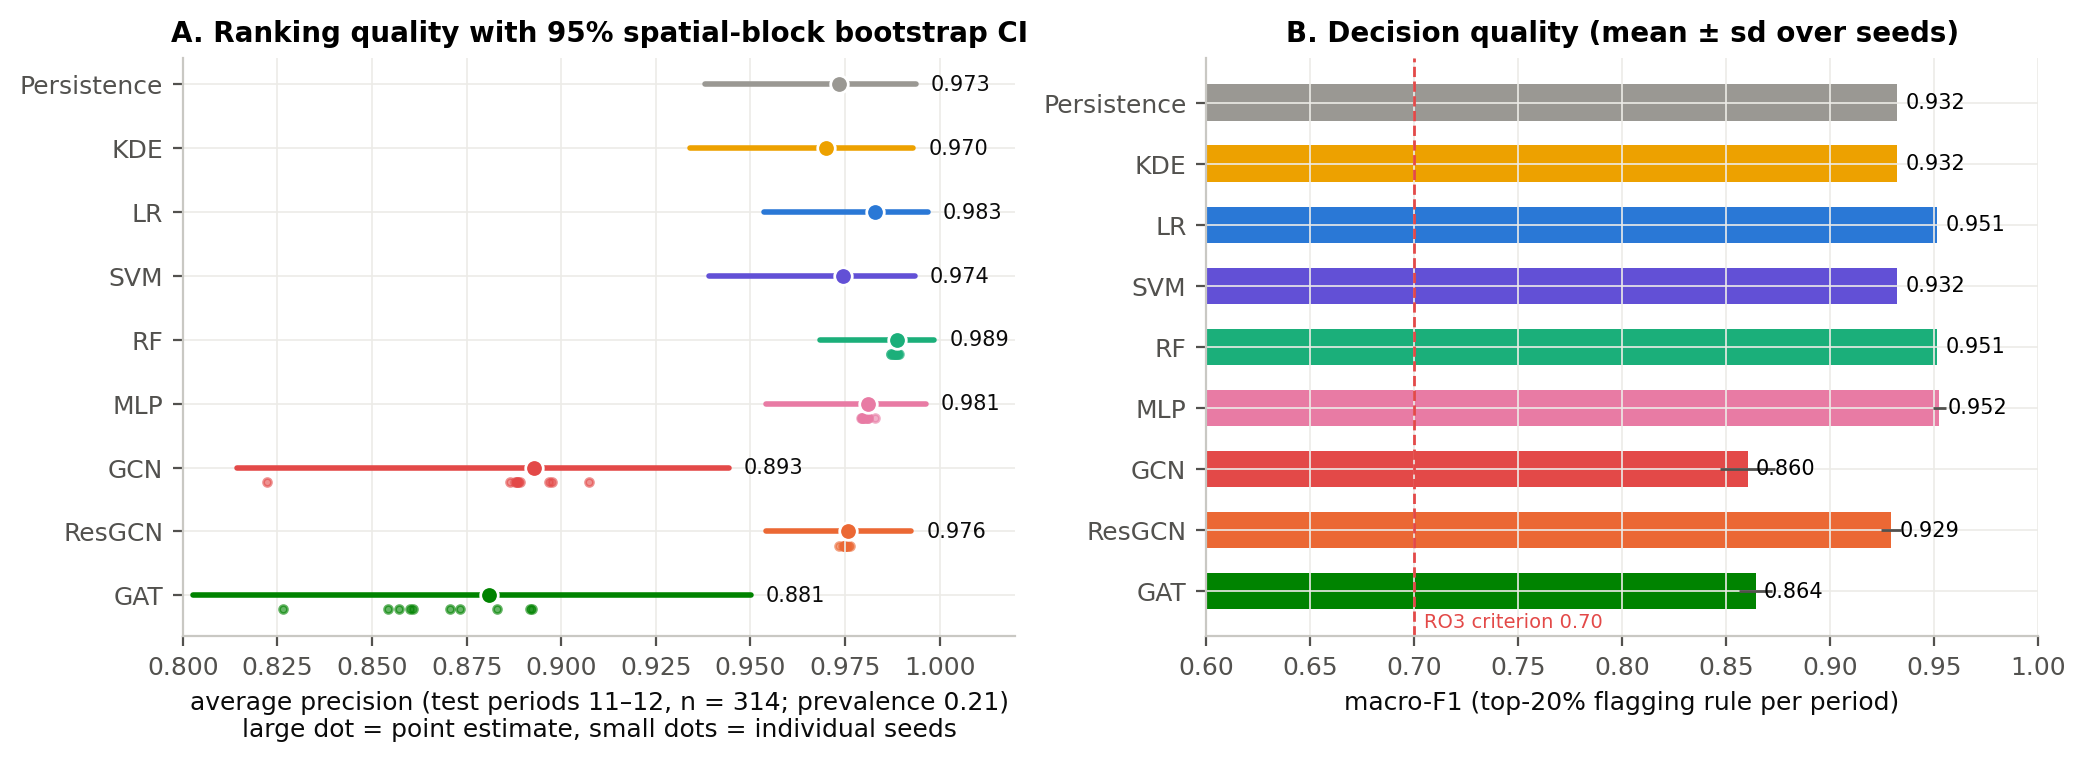
\includegraphics[width=\textwidth]{F05_p2_comparison.png}
\caption{Phase~2 test comparison. (A) AP with 95\% spatial-block bootstrap intervals; small dots show individual seeds. (B) Macro-F1 under the operational top-20\% rule; the dashed line is the RO3 criterion.}
\label{fig:p2}
\end{figure}

LR was chosen as the Phase~2 classifier based on the pre-stated criterion because it had the highest validation AP (0.968) of all models. The test confusion matrix for the top-20\% rule (Figure~\ref{fig:cm}) for LR is 244 true negatives, 4 false positives, 6 false negatives, and 60 true positives; precision 0.938 and recall 0.909 for the high class. Since the rule selects exactly 32 cells per period but there are 32--35 cells that are marked high (ties), some false negatives are inherent to the problem, as even a perfect ranking would miss the ties past the 32nd cell.

\begin{figure}[H]
\centering
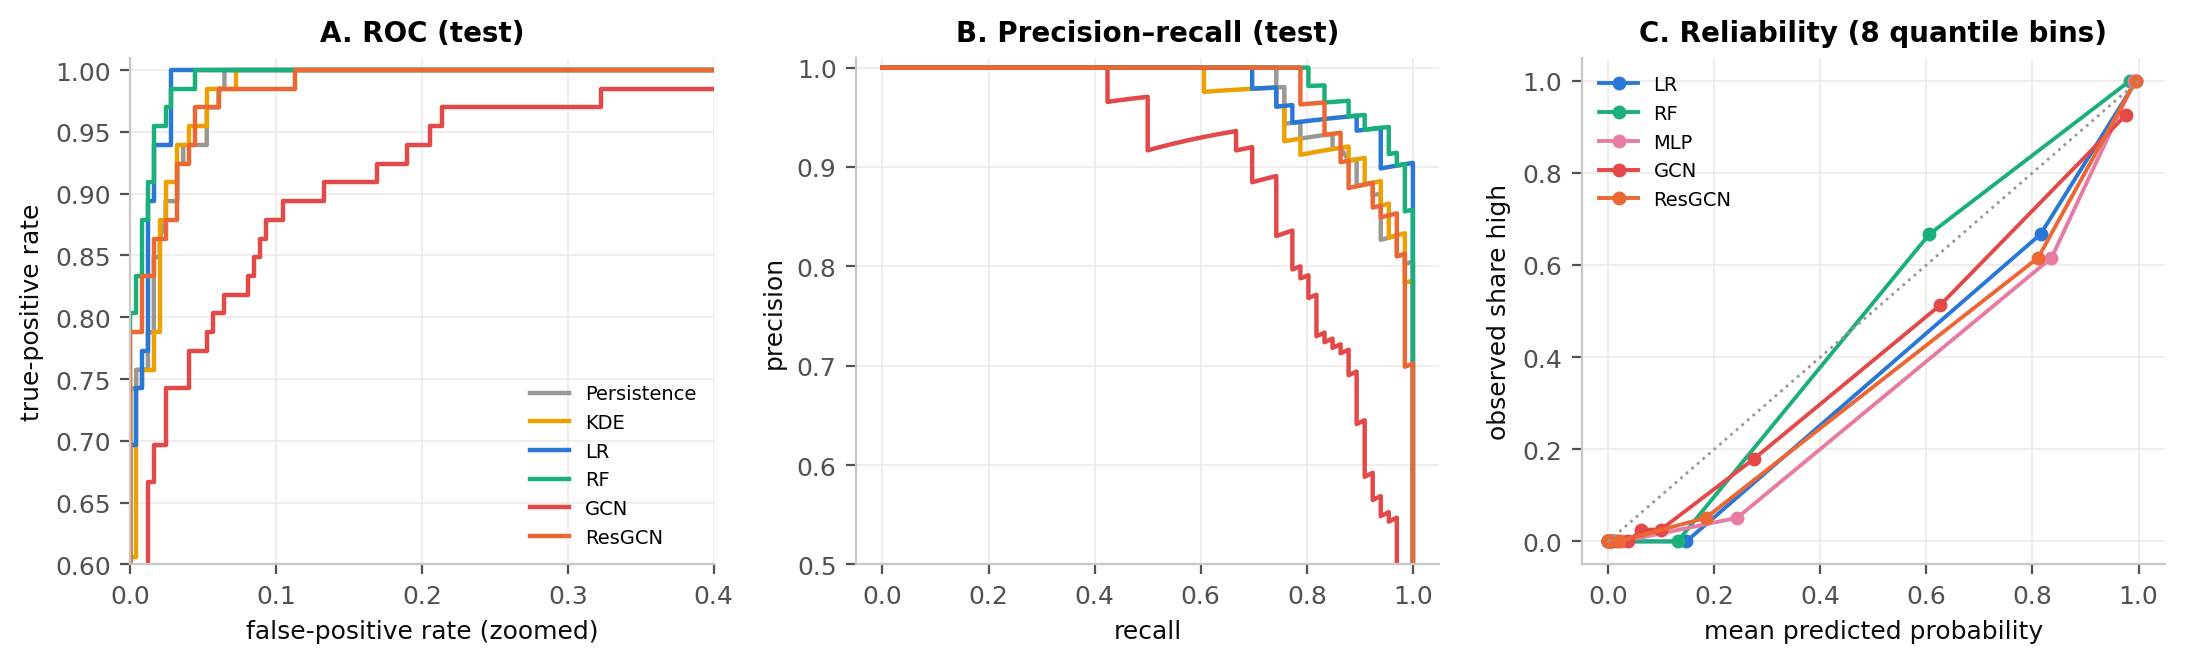
\includegraphics[width=\textwidth]{F06_roc_pr_calibration.png}
\caption{Phase~2 test ROC curves (zoomed), precision--recall curves and reliability diagrams. Persistence and KDE are ranking scores, so they have no reliability curve.}
\label{fig:rocpr}
\end{figure}

The curves in Figure~\ref{fig:rocpr} show the same ranking. The GCN's precision drops sharply beyond 50\% recall, indicating that it confuses moderately high cells with their neighbours. The reliability diagram suggests that LR and the MLP are slightly overconfident in the 0.6--0.9 range---an expected effect of class weighting, which shifts probabilities upward---while RF is closest to the diagonal (Brier 0.023). Calibration matters for the application only if probabilities are displayed; therefore, the design presents ranks and calibrated bands rather than raw probabilities (Section~\ref{sec:app}).


\subsection{Phase 1: Dominant Crime Type (E3)}
\label{sec:p1res}
Forecasting the dominant type was much more challenging (Table~\ref{tab:p1}). The majority-class baseline (\textsc{battery}) achieves a macro-F1 of 0.134; persistence achieves 0.404; and LR achieves 0.498, the highest test macro-F1. The GCN achieves $0.450\pm0.019$  and the GAT $0.450\pm0.010$, both below the SVM (0.467). The validation criterion selected the MLP (validation macro-F1 of 0.520 compared with 0.492 for LR), which achieved $0.482\pm0.018$ on the test periods. LR's higher test score falls within the MLP's seed range and bootstrap interval, so their performance could not be distinguished in this evaluation. RQ1 is therefore answered negatively: the GCN did not outperform the SVM or the non-graph MLP.

\begin{table}[H]
\centering\scriptsize
\caption{Phase~1 test results (periods 11--12; $n=303$; support: battery 136, criminal damage 27, theft 111, other 29). Mean $\pm$ sd over 10 seeds where stochastic}
\label{tab:p1}
\resizebox{\textwidth}{!}{\begin{tabular}{@{}lcccccccc@{}}
\toprule
Model & Accuracy & Macro-F1 & Weighted F1 & $\kappa$ & F1 battery & F1 crim.\ damage & F1 theft & F1 other\\
\midrule
Majority & 0.366 & 0.134 & 0.196 & 0.000 & 0.000 & 0.000 & 0.536 & 0.000\\
Persistence & 0.604 & 0.404 & 0.580 & 0.363 & 0.705 & 0.054 & 0.655 & 0.200\\
KDE & \textbf{0.640} & 0.426 & 0.608 & 0.413 & 0.715 & 0.061 & \textbf{0.711} & 0.217\\
\textbf{LR} & 0.611 & \textbf{0.498} & \textbf{0.630} & 0.425 & \textbf{0.743} & \textbf{0.265} & 0.660 & 0.324\\
SVM & 0.564 & 0.467 & 0.597 & 0.388 & 0.717 & 0.192 & 0.615 & 0.344\\
RF & $0.629\pm0.007$ & $0.460\pm0.008$ & 0.621 & \textbf{0.437} & 0.738 & 0.006 & 0.681 & \textbf{0.418}\\
MLP (val.\ selected) & $0.593\pm0.013$ & $0.482\pm0.018$ & 0.622 & 0.418 & 0.737 & 0.170 & 0.659 & 0.363\\
GCN & $0.547\pm0.016$ & $0.450\pm0.019$ & 0.583 & 0.360 & 0.711 & 0.154 & 0.593 & 0.343\\
ResGCN & $0.567\pm0.021$ & $0.467\pm0.025$ & 0.600 & 0.383 & 0.692 & 0.166 & 0.656 & 0.353\\
GAT & $0.550\pm0.012$ & $0.450\pm0.010$ & 0.584 & 0.362 & 0.715 & 0.163 & 0.592 & 0.331\\
\bottomrule
\end{tabular}}
\end{table}

The per-class results indicate why this is difficult. \textsc{Battery} and \textsc{theft} are reasonably well predicted (F1 0.66 to 0.74) as there are a large number of cells where one type dominates consistently. However, \textsc{Criminal damage} is the dominant type in just 27 test cell-periods, and even when it is the dominant type it is usually only narrowly leading theft or battery, so even the best model gets an F1 of 0.27; RF effectively never predicts it. The confusion matrices (Figure~\ref{fig:cm}) reveal that persistence tends to confuse \textsc{battery} and \textsc{theft} the most (30 and 23 swaps), since both counts in mixed cells are similar. LR sacrifices some \textsc{theft} accuracy for more recall on the two minority classes, which explains why its accuracy is lower than that of KDE, but its macro-F1 is higher. The error map (Fig.~\ref{fig:errmap}B) indicates that Phase~1 errors are located mostly in the north-west and far south, where the cells have low volumes and mixed profiles, while the dense cells in the centre and south with a clear battery or theft profile are hardly ever wrong.


\begin{figure}[H]
\centering
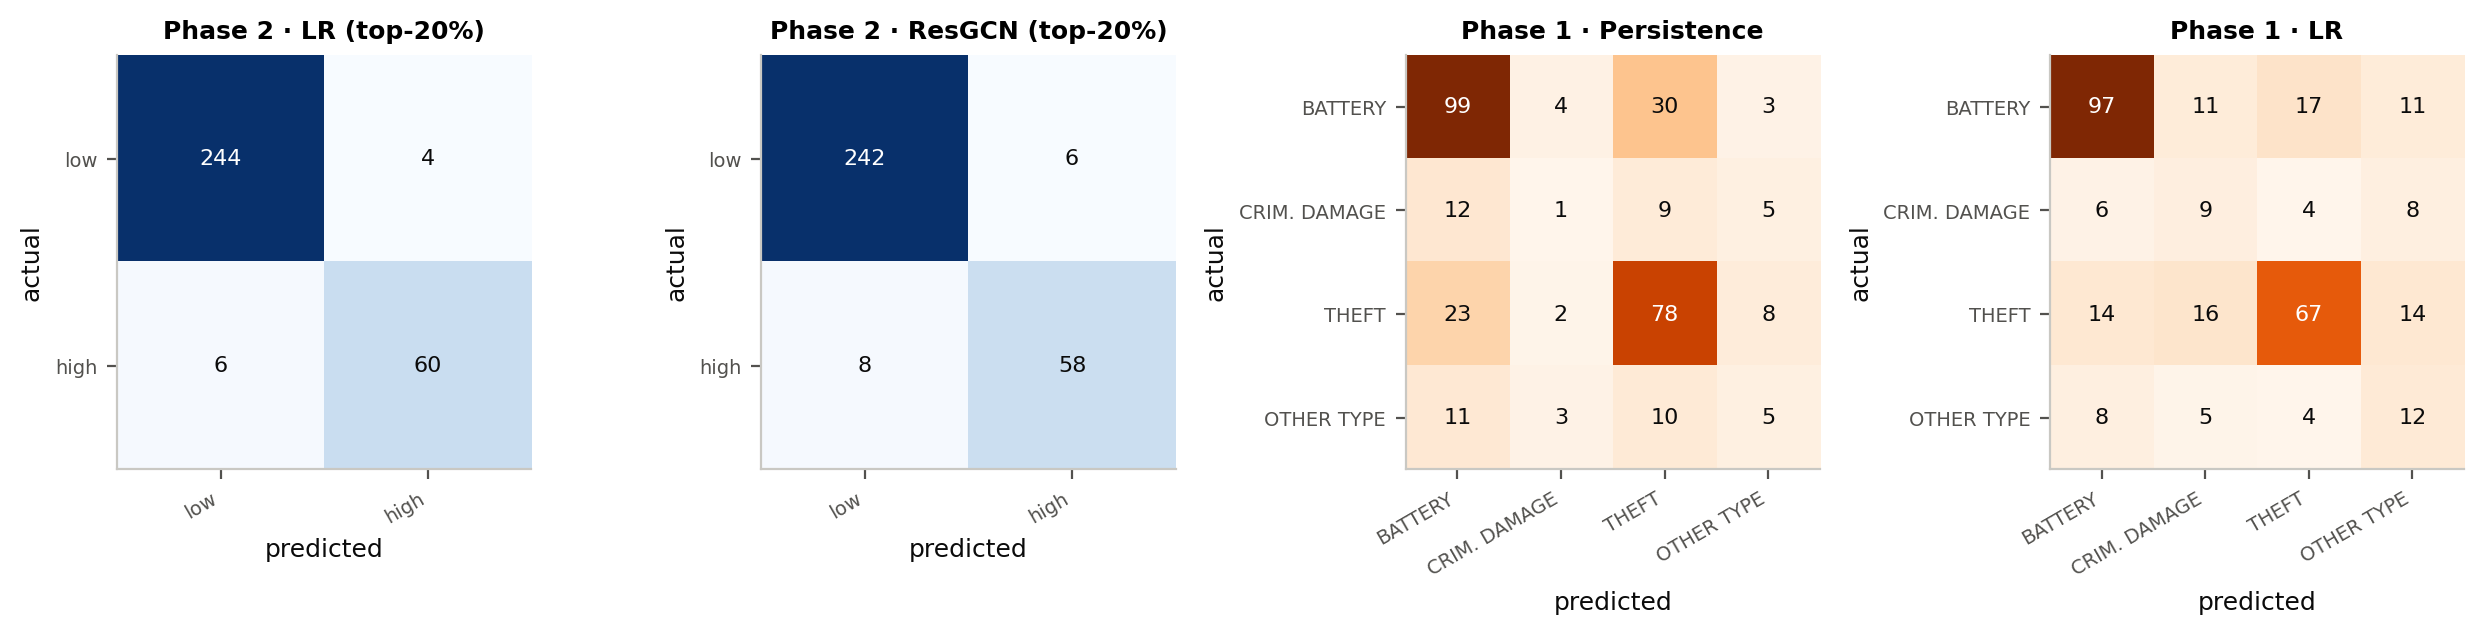
\includegraphics[width=\textwidth]{F07_confusion.png}
\caption{Test confusion matrices: Phase~2 under the top-20\% rule (LR, ResGCN) and Phase~1 (persistence, LR).}
\label{fig:cm}
\end{figure}

\begin{figure}[H]
\centering
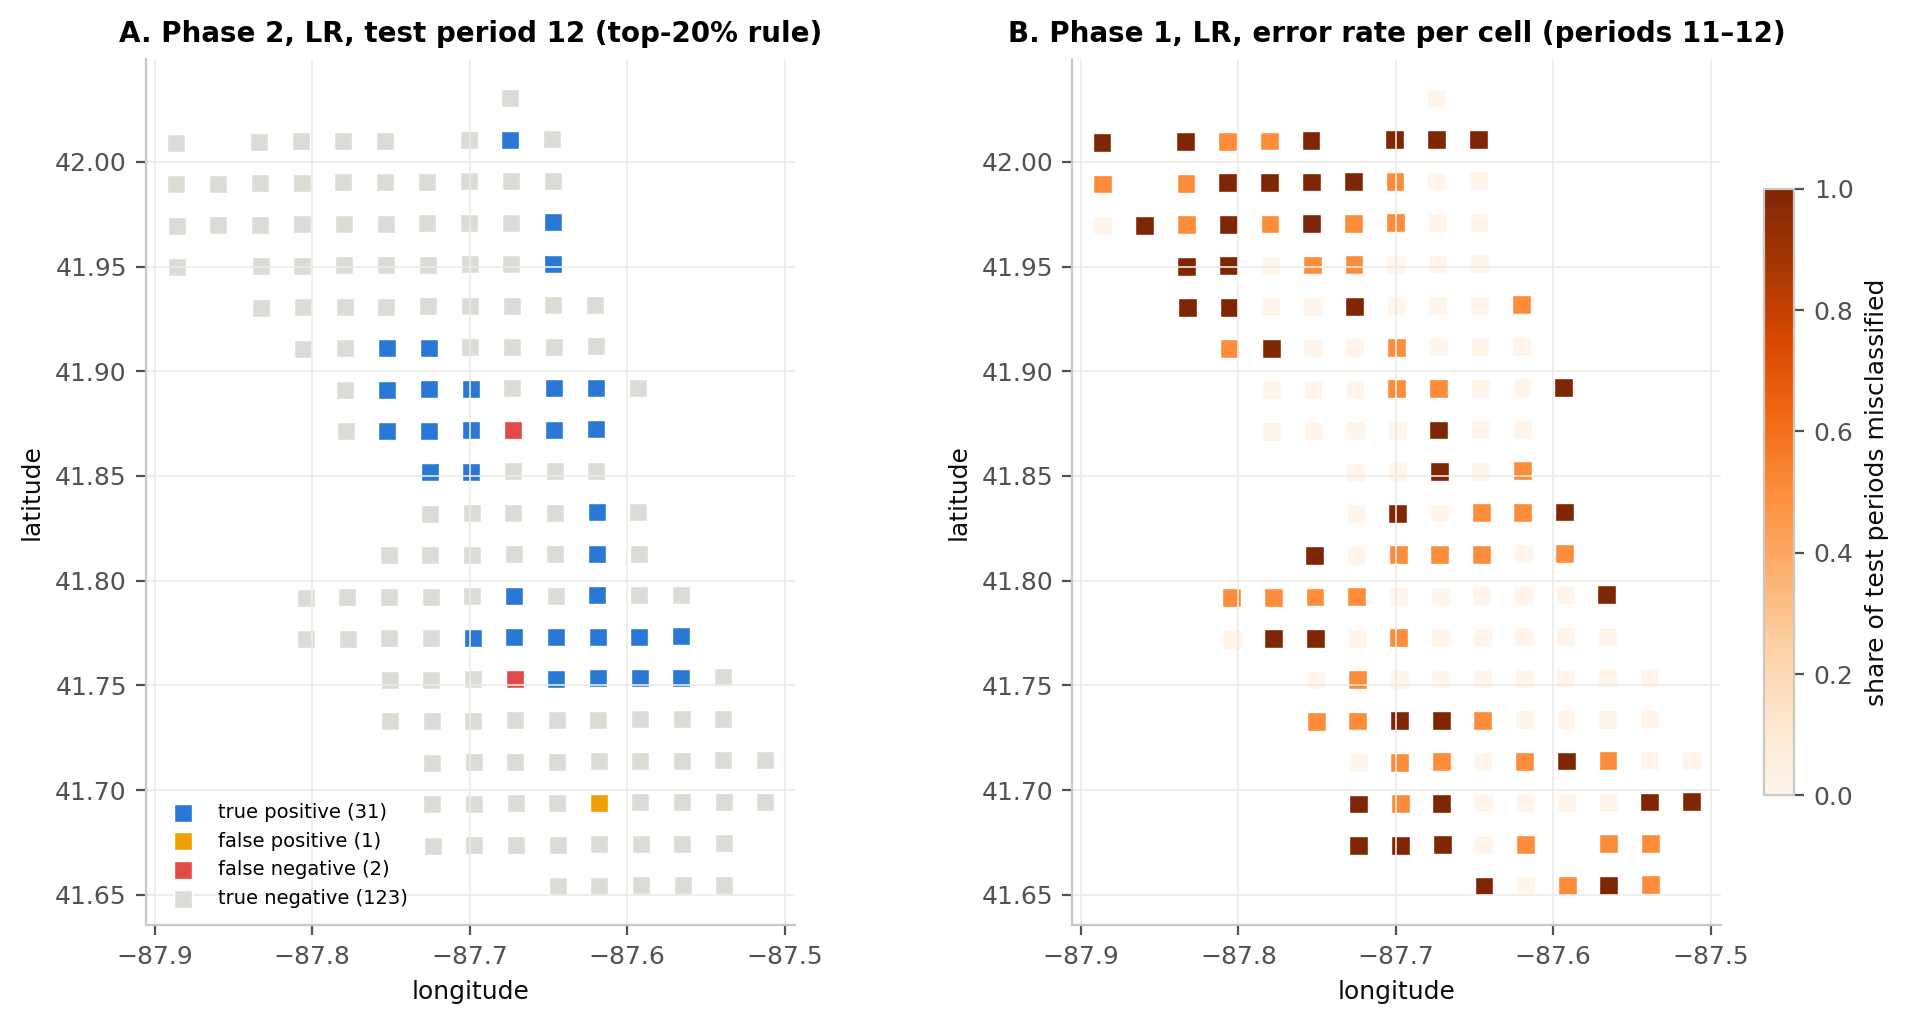
\includegraphics[width=\textwidth]{F11_error_maps.png}
\caption{Geographic error analysis on test periods. (A) Phase~2 LR outcomes in period 12. (B) Share of the two test periods in which LR misclassified each cell's dominant type.}
\label{fig:errmap}
\end{figure}

Phase~2 errors are rare and exist on the edge of the high category (Figure~\ref{fig:errmap}A). During period~12, the threshold was 71 incidents: one false negative (86 incidents), which was ranked 33rd, just outside the top 32 cells, and another, which was exactly equal to the threshold value of 71; the single false positive, a far-south cell with a high past volume, recorded 61 incidents and was ranked 31st. No geographic area is systematically missed, although evidence is available for only two testing episodes.

\subsection{Class-Imbalance Strategies (E4)}
\begin{table}[H]
\centering\small
\caption{Imbalance strategies for Phase~2 (test). Threshold metrics depend on the decision threshold; AP does not}
\label{tab:imb}
\begin{tabular}{@{}llccccc@{}}
\toprule
Strategy & Threshold & AP & Precision & Recall & Pos.\ F1 & Macro-F1\\
\midrule
LR, no weighting & 0.5 & 0.985 & 0.926 & 0.955 & 0.940 & 0.962\\
LR, no weighting & validation-tuned & 0.985 & 0.868 & 1.000 & 0.930 & 0.955\\
LR, class weights & 0.5 & 0.983 & 0.868 & 1.000 & 0.930 & 0.955\\
LR, class weights & validation-tuned & 0.983 & 0.944 & 0.773 & 0.850 & 0.907\\
LR, SMOTE (train only) & 0.5 & 0.985 & 0.892 & 1.000 & 0.943 & 0.963\\
LR, SMOTE (train only) & validation-tuned & 0.985 & 0.948 & 0.833 & 0.887 & 0.930\\
GCN, unweighted CE & 0.5 & 0.881 & 0.922 & 0.647 & 0.760 & 0.854\\
GCN, weighted CE & 0.5 & 0.885 & 0.738 & 0.824 & 0.765 & 0.841\\
GCN, weighted CE & validation-tuned & 0.885 & 0.870 & 0.717 & 0.784 & 0.866\\
\bottomrule
\end{tabular}
\end{table}
There are three points to note about Table~\ref{tab:imb}. First, none of the strategies modified the ranking quality, with LR's AP varying between 0.983 and 0.985, as reweighting mostly affects the intercept. Second, the strategies modified the precision-recall trade-off for a given threshold, such that class weighting and SMOTE gave LR perfect recall at the cost of precision, and class weighting shifted the GCN's recall from 0.647 to 0.824. Third, optimising the threshold on only two validation periods harmed all LR variants on the test periods (e.g., macro-F1 0.955 $\to$ 0.907 with class weights) because the F1-optimal threshold on 314 validation samples is noisy. In the three-year replication (948 validation samples), this depends on the validation sample size: the optimised threshold was either neutral or beneficial (unweighted LR 0.917 $\to$ 0.934; class-weighted LR 0.935 $\to$ 0.933; SMOTE 0.933 $\to$ 0.927; weighted GCN 0.859 $\to$ 0.862), and class weighting again affected recall (unweighted LR 0.828, weighted 0.932) but not AP (0.959 vs 0.958). Thus, the application will use a prevalence-matched top-$k$ strategy that requires no parameter tuning and can be recalculated each period, and will take into account a tuned threshold only after about six closed validation periods have been completed. There were no gains from SMOTE over class weights in either study, so class weights were used.


\subsection{Graph Ablations: When Does Message Passing Help? (E5)}
\label{sec:ablation}
\begin{table}[H]
\centering\scriptsize
\caption{Graph ablations (test; mean $\pm$ sd over 10 seeds). Pilot-style GCN versus residual GCN}
\label{tab:abl}
\resizebox{\textwidth}{!}{\begin{tabular}{@{}lrr cc cc@{}}
\toprule
 & & & \multicolumn{2}{c}{Phase 2 AP} & \multicolumn{2}{c}{Phase 1 macro-F1}\\
\cmidrule(lr){4-5}\cmidrule(lr){6-7}
Graph / depth & Edges & Mean degree & GCN & ResGCN & GCN & ResGCN\\
\midrule
Rook 3.0~km, inverse distance (pilot) & 272 & 3.5 & $0.885\pm0.023$ & $0.975\pm0.001$ & $0.450\pm0.019$ & $0.467\pm0.025$\\
Rook 3.0~km, unweighted & 272 & 3.5 & $0.870\pm0.029$ & $0.974\pm0.002$ & $0.448\pm0.011$ & $0.464\pm0.020$\\
Queen 3.2~km, inverse distance & 528 & 6.7 & $0.848\pm0.024$ & $0.973\pm0.001$ & $0.441\pm0.012$ & $0.461\pm0.026$\\
Radius 4.5~km, inverse distance & 765 & 9.7 & $0.779\pm0.018$ & $0.975\pm0.001$ & $0.426\pm0.020$ & $0.460\pm0.020$\\
Radius 6.6~km, inverse distance & 1,640 & 20.9 & $0.729\pm0.010$ & $0.976\pm0.001$ & $0.386\pm0.014$ & $0.450\pm0.022$\\
\midrule
Depth 1 (rook) & 272 & 3.5 & $0.893\pm0.009$ & $0.959\pm0.021$ & $0.453\pm0.013$ & $0.474\pm0.024$\\
Depth 2 (rook) & 272 & 3.5 & $0.885\pm0.023$ & $0.975\pm0.001$ & $0.450\pm0.019$ & $0.467\pm0.025$\\
Depth 3 (rook) & 272 & 3.5 & $0.872\pm0.011$ & $0.973\pm0.003$ & $0.429\pm0.016$ & $0.466\pm0.017$\\
\midrule
MLP (no graph) & 0 & 0 & \multicolumn{2}{c}{$0.980\pm0.001$} & \multicolumn{2}{c}{$0.482\pm0.018$}\\
LR without / with spatial-lag features & -- & -- & \multicolumn{2}{c}{0.983 / 0.983} & \multicolumn{2}{c}{--}\\
\bottomrule
\end{tabular}}
\end{table}

\begin{figure}[H]
\centering
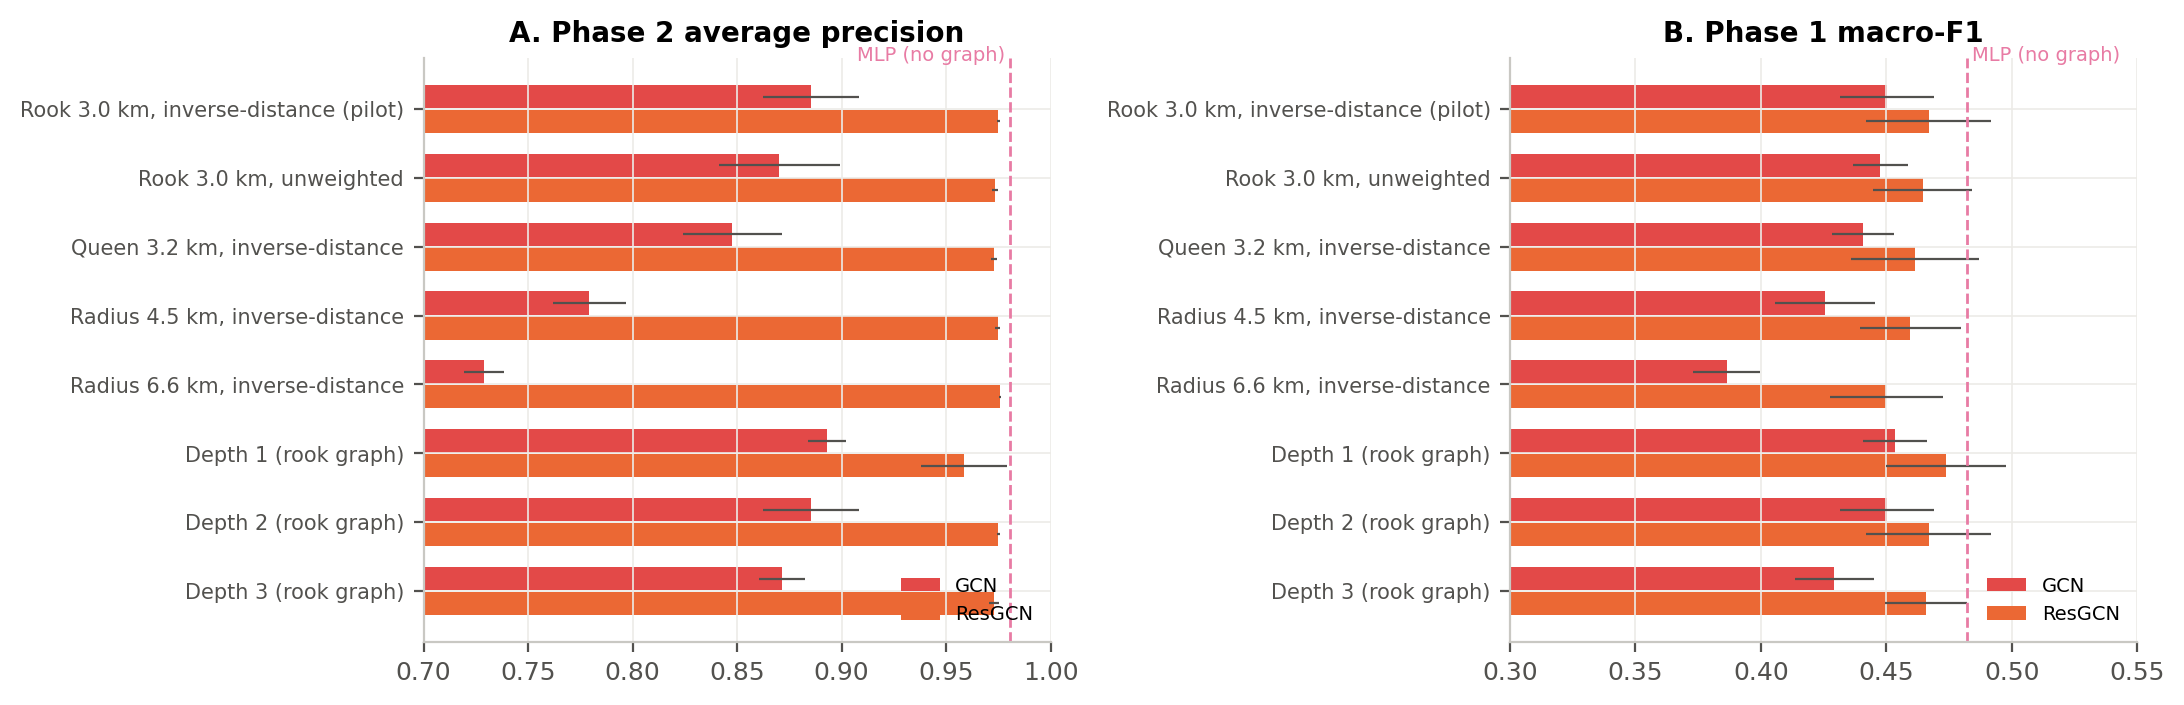
\includegraphics[width=\textwidth]{F09_graph_ablation.png}
\caption{Graph ablations. The degradation in performance by the GCN increases as neighbourhood size and layer count increase, while the residual GCN becomes independent of the graph structure, approaching, but not exceeding, the MLP.}
\label{fig:abl}
\end{figure}

The ablation results (Table~\ref{tab:abl}, Figure~\ref{fig:abl}) support the smoothing hypothesis of Section~\ref{sec:transform}. The AP of the baseline GCN model decreases monotonically from 0.885 to 0.729 with the increase of the mean degree from 3.5 to 20.9 and decreases with each additional layer, which is exactly what is predicted by the self-weight $1/(d_i+1)$ and by the Laplacian-smoothing interpretation of \citet{li2018}. The elimination of the inverse distance weights made little difference (0.885 compared with 0.870 within one seed standard deviation), demonstrating that the uniform weights did not have any information content. The residual graph convolutional network, whose self connection is not weakened by degree, stayed flat on all of the graphs (0.973--0.976): it had learned to utilise each cell's past only and the neighbour connection contributed nothing measurable. Its pairwise difference from the MLP is $-0.004$ average precision (95\% confidence interval $[-0.013, 0.008]$; Table~\ref{tab:boot}). Adding neighbour-average features to LR also left AP unchanged (0.9830 vs 0.9834 AP). Across three independent tests, therefore, information from neighbouring cells did not improve forecasts once a cell's own history was known.


\subsection{Feature Ablation and Leakage Check (E6)}
\begin{table}[H]
\centering\small
\caption{Feature-group ablation (test). GCN values are means over five seeds}
\label{tab:feat}
\begin{tabular}{@{}lrcccc@{}}
\toprule
 & & \multicolumn{2}{c}{Phase 2 AP} & \multicolumn{2}{c}{Phase 1 macro-F1}\\
\cmidrule(lr){3-4}\cmidrule(lr){5-6}
Feature set & Features & LR & GCN & LR & GCN\\
\midrule
All features & 23 & 0.983 & 0.896 & 0.498 & 0.448\\
Without victimisation history & 17 & 0.974 & 0.895 & 0.502 & 0.443\\
Without crime-mix shares & 15 & 0.983 & 0.932 & 0.493 & 0.457\\
Without coordinates & 21 & 0.982 & 0.847 & 0.507 & 0.454\\
Victimisation lags only & 4 & \textbf{0.991} & 0.867 & 0.340 & 0.391\\
\bottomrule
\end{tabular}
\end{table}
Table~\ref{tab:feat} indicates that Phase~2 predictive performance comes almost entirely from victimisation history: four lagged features alone give LR an AP of 0.991, exceeding the full feature set (0.983). This suggests that the additional features may add a little variance without contributing further predictive signal. Removing victimisation history reduces LR's AP by only 0.009 because total-crime lags contain much of the same information. Phase~1 shows the opposite pattern: removing crime-mix shares barely changes LR's macro-F1 (0.493), whereas using victimisation lags alone reduces it to 0.340. This suggests that crime-type forecasting relies on the combined feature profile rather than any single feature group. Since all the features come before the target period, none of these results depends on leakage; the comparison with the pilot's perfect argmax rule (Table~\ref{tab:pilot}) reveals the extent to which a circular design would have exaggerated skill. The GCN benefits from excluding the composition shares (0.896 $\to$ 0.932), further evidence that aggregation mixes cell-level information with that of neighbours.


\subsection{Robustness over Time, Space, Labels and Resolution (E7--E9)}
\label{sec:robust}
\begin{table}[H]
\centering\small
\caption{Rolling-origin evaluation: Phase~2 AP (top) and Phase~1 macro-F1 (bottom) by test period; each model is retrained on all earlier periods}
\label{tab:roll}
\begin{tabular}{@{}lccccc@{}}
\toprule
Test period & 8 & 9 & 10 & 11 & 12\\
Training target periods & 3--6 & 3--7 & 3--8 & 3--9 & 3--10\\
\midrule
P2 Persistence & 0.938 & 0.965 & \textbf{0.969} & 0.970 & 0.977\\
P2 KDE & 0.909 & 0.944 & 0.932 & 0.952 & \textbf{0.991}\\
P2 LR & \textbf{0.944} & 0.962 & 0.960 & \textbf{0.977} & \textbf{0.991}\\
P2 GCN (5 seeds) & 0.854 & 0.860 & 0.882 & 0.885 & 0.949\\
P2 ResGCN (5 seeds) & 0.935 & \textbf{0.965} & 0.941 & 0.965 & 0.987\\
\midrule
P1 Persistence & \textbf{0.458} & \textbf{0.446} & 0.390 & 0.425 & 0.382\\
P1 LR & 0.425 & 0.428 & \textbf{0.567} & \textbf{0.490} & 0.460\\
P1 GCN (5 seeds) & 0.431 & 0.391 & 0.456 & 0.444 & \textbf{0.472}\\
\bottomrule
\end{tabular}
\end{table}

\begin{figure}[H]
\centering
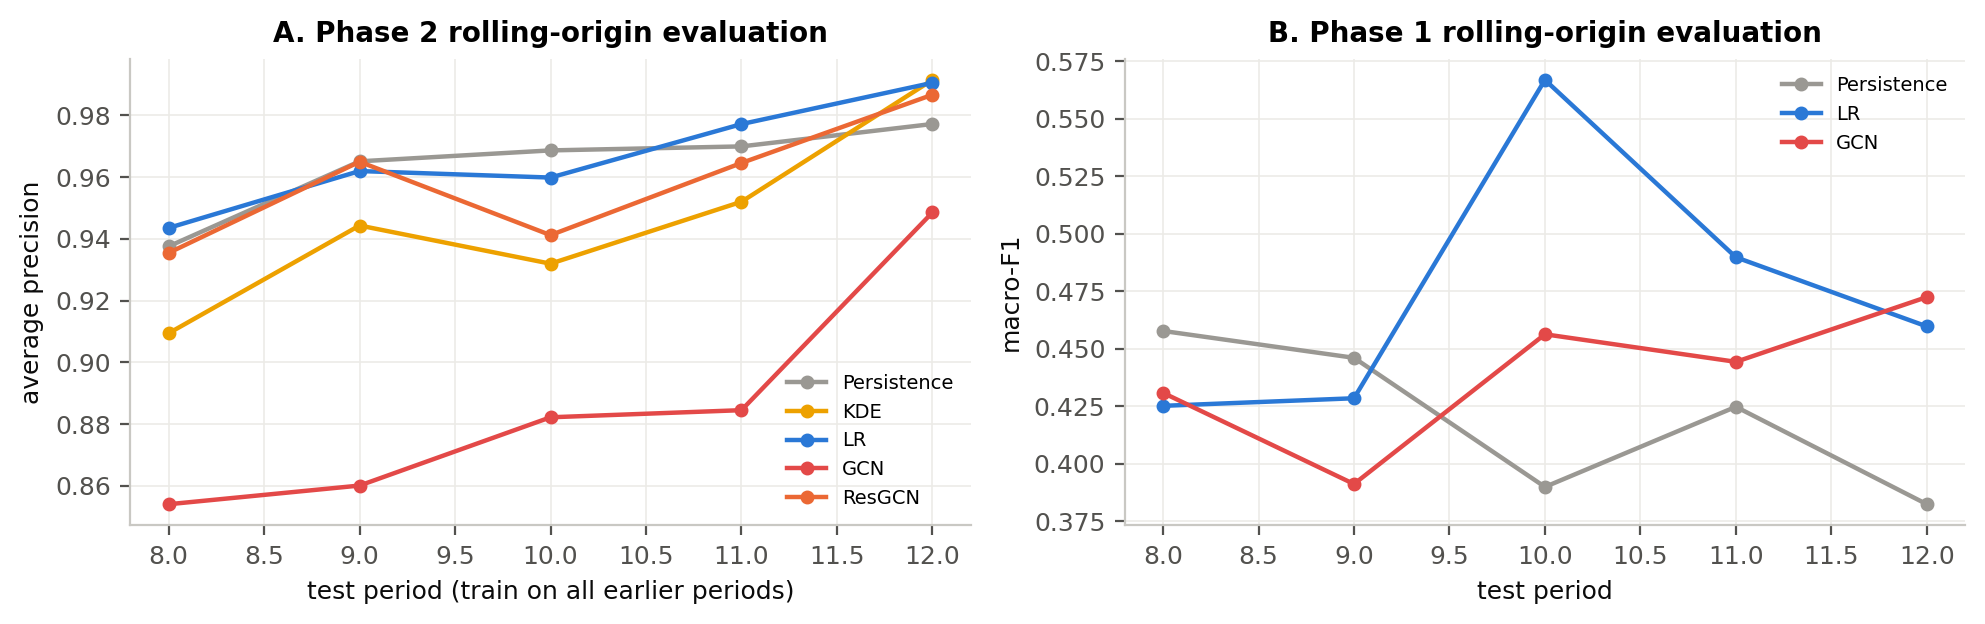
\includegraphics[width=\textwidth]{F10_rolling_origin.png}
\caption{Rolling-origin evaluation across five test periods.}
\label{fig:roll}
\end{figure}

\paragraph{Over time.} The rolling origin (Table~\ref{tab:roll}, Figure~\ref{fig:roll}) reveals that the Phase~2 ranking is stable: LR and persistence are within 0.01 AP of each other in four out of five windows, the GCN is the worst in all five windows, and all models get better as more training data becomes available and as summer volumes increase. LR outperforms persistence in three out of five windows, so its superiority is slight and inconsistent. The Phase~1 ranking is unstable: persistence outperforms in the first two windows (when LR has only four training periods), LR wins periods 10 and 11, while the GCN wins period 12. Conclusions drawn from Phase~1 should hence be considered tentative.

\begin{table}[H]
\centering\small
\caption{Spatial-block cross-validation for Phase~2: held-out cells' labels masked during training; AP on held-out cells in test periods}
\label{tab:block}
\begin{tabular}{@{}cccccccc@{}}
\toprule
Block & Cells & Test rows (high) & Persistence & LR & MLP & GCN & ResGCN\\
\midrule
0 & 29 & 58 (10) & 0.973 & 1.000 & 0.994 & 0.953 & 0.983\\
1 & 26 & 52 (10) & 0.933 & 0.981 & 0.914 & 0.634 & 0.938\\
2 & 37 & 74 (13) & 0.995 & 0.989 & 0.958 & 0.828 & 0.936\\
3 & 30 & 60 (2) & 1.000 & 1.000 & 1.000 & 0.667 & 1.000\\
4 & 35 & 70 (31) & 0.983 & 0.984 & 0.986 & 0.863 & 0.974\\
\midrule
Mean & & & 0.977 & \textbf{0.991} & 0.970 & 0.789 & 0.966\\
\bottomrule
\end{tabular}
\end{table}

\paragraph{Over space.} Holding out entire regions (Table~\ref{tab:block}) is the most difficult challenge for a graph model since the held-out cells' labels are unknown, but the features of their neighbours are known. LR transferred best (mean AP = 0.991), but the GCN performance declined sharply in blocks 1 and 3 (AP = 0.634 and 0.667). Block~3, located in the far south, contains only two high cell-periods, so its AP is highly unreliable and should not be over-interpreted. This indicates that the GCN's learning of smoothing does not transfer to regions with unfamiliar spatial structure, unlike history-based tabular models.

\begin{figure}[H]
\centering
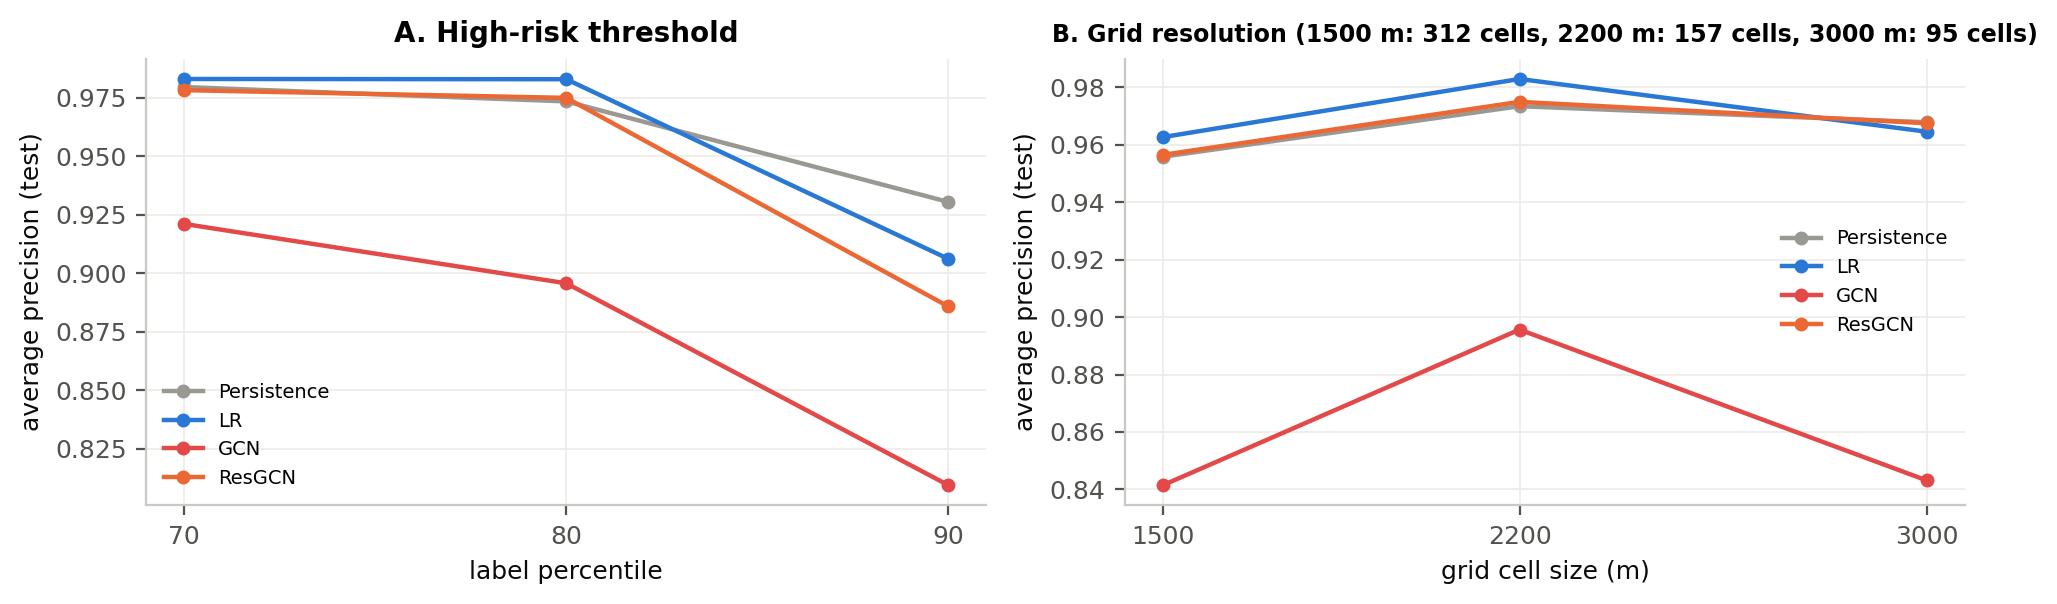
\includegraphics[width=\textwidth]{F13_sensitivity.png}
\caption{Sensitivity of Phase~2 test AP to the label percentile and to grid resolution.}
\label{fig:sens}
\end{figure}

\paragraph{Label threshold and grid size.} Figure~\ref{fig:sens} and Appendix Table~\ref{tab:sens} show that the conclusions are robust to the labelling choice: at the 70th percentile threshold (prevalence=0.30), all models apart from GCN have AP=0.978-0.983; at the 90th percentile (prevalence=0.10) AP is lowered for all models, with persistence (AP=0.930) ahead of logistic regression (AP=0.906), as the top decile represents a very stable population. When using cell sizes of 1.5~km (number of cells=312) and 3.0~km (number of cells=95), the ordering was maintained; namely, persistence, LR and ResGCN were within 0.01 of one another, with GCN lower by 0.09-0.13 AP relative to LR for each resolution tested. Finer grids result in a slight AP decline (0.956-0.963 at 1.5~km) because counts per cell are noisier.

\subsection{Statistical Uncertainty and Paired Comparisons (E10)}
\begin{table}[H]
\centering\small
\caption{Spatial-block bootstrap (26 blocks of $3\times3$ cells, 2,000 resamples) for paired differences on the test periods}
\label{tab:boot}
\begin{tabular}{@{}lccc@{}}
\toprule
Comparison & Mean difference & 95\% CI & Share of resamples $>0$\\
\midrule
P2 AP: LR $-$ Persistence & $+0.009$ & $[-0.008, 0.031]$ & 0.86\\
P2 AP: RF $-$ LR & $+0.006$ & $[-0.002, 0.021]$ & 0.93\\
P2 AP: GCN $-$ LR & $-0.090$ & $[-0.152, -0.046]$ & 0.00\\
P2 AP: GCN $-$ MLP & $-0.089$ & $[-0.154, -0.046]$ & 0.00\\
P2 AP: ResGCN $-$ GCN & $+0.085$ & $[0.039, 0.154]$ & 1.00\\
P2 AP: ResGCN $-$ MLP & $-0.004$ & $[-0.013, 0.008]$ & 0.17\\
P2 AP: ResGCN $-$ LR & $-0.005$ & $[-0.018, 0.012]$ & 0.22\\
P2 AP: GAT $-$ MLP & $-0.098$ & $[-0.163, -0.039]$ & 0.00\\
P2 AP: GAT $-$ GCN & $-0.009$ & $[-0.059, 0.056]$ & 0.33\\
P1 macro-F1: LR $-$ Persistence & $+0.092$ & $[0.006, 0.167]$ & 0.98\\
P1 macro-F1: GCN $-$ Persistence & $+0.038$ & $[-0.037, 0.103]$ & 0.85\\
\bottomrule
\end{tabular}
\end{table}
Table~\ref{tab:boot} provides the answer to RQ3. Resampling blocks of 6.6~km instead of individual cell-periods takes into account spatial correlation; in the case of the GCN, the confidence interval for AP ($[0.814, 0.944]$) is wider than under the naive independent bootstrap ($[0.831, 0.944]$), as expected when neighbouring errors are correlated. Three differences are clearly real: the GCN is inferior to the LR and the MLP models by about 0.09 AP, the residual GCN is superior to the GCN by 0.085, the GAT is inferior to the MLP model by about 0.10 AP, and the superiority of LR over persistence in terms of crime type (+0.09 macro-F1, interval $[0.006, 0.167]$) is marginal and not confirmed by the permutation test (raw $p=0.077$, Table~\ref{tab:perm}). Three are not distinguishable from zero: LR vs. Persistence for victimisation, RF vs. LR, and ResGCN vs. MLP. The bootstrap accounts for uncertainty due to which neighbourhoods happened to be tested; seed uncertainty is given in Tables~\ref{tab:p2}--\ref{tab:p1}, and temporal uncertainty by the rolling origin. Because the intervals rely on only two test periods, they still understate uncertainty about future seasons. As intervals alone cannot form a test, E16 adds paired spatial-block permutation tests with Holm adjustment (Table~\ref{tab:perm}), so effect sizes with intervals are treated as the principal evidence since the 26 blocks provide the test with limited power and lack of significance does not indicate equivalence.

\subsection{Continuous Count Forecasting (E11)}
\begin{table}[H]
\centering\small
\caption{Next-period victimisation count forecasts (test; $n=314$)}
\label{tab:reg}
\begin{tabular}{@{}lcccc@{}}
\toprule
Model & MAE & RMSE & $R^2$ & Spearman $\rho$\\
\midrule
Persistence (last period) & 6.59 & 9.54 & 0.939 & 0.973\\
Persistence (3-period mean) & 5.99 & \textbf{8.62} & \textbf{0.950} & \textbf{0.979}\\
Poisson GLM ($\alpha=1$) & \textbf{5.95} & 8.94 & 0.946 & \textbf{0.979}\\
MLP (Poisson loss, 5 seeds) & 6.70 & 9.98 & 0.933 & 0.977\\
GCN (Poisson loss, 5 seeds) & 11.55 & 16.80 & 0.810 & 0.912\\
\bottomrule
\end{tabular}
\end{table}
The continuous task promised in Assessment~1 validates the classification results (Table~\ref{tab:reg}). A three-period moving average accounts for 95\% of the variance in next-period counts and ties with, but does not outperform, a Poisson GLM. The GCN using a Poisson loss function performs significantly worse. Since the neural count models used the same hyperparameters as the classifiers and the GLM $\alpha$ was on the border of its grid, both were investigated later in E18 (Section~\ref{sec:posthoc}), with tuned neural models and a larger $\alpha$ grid, and the conclusion did not change.

\subsection{Unsupervised Hotspot Detection with DBSCAN (E12)}
\begin{figure}[H]
\centering
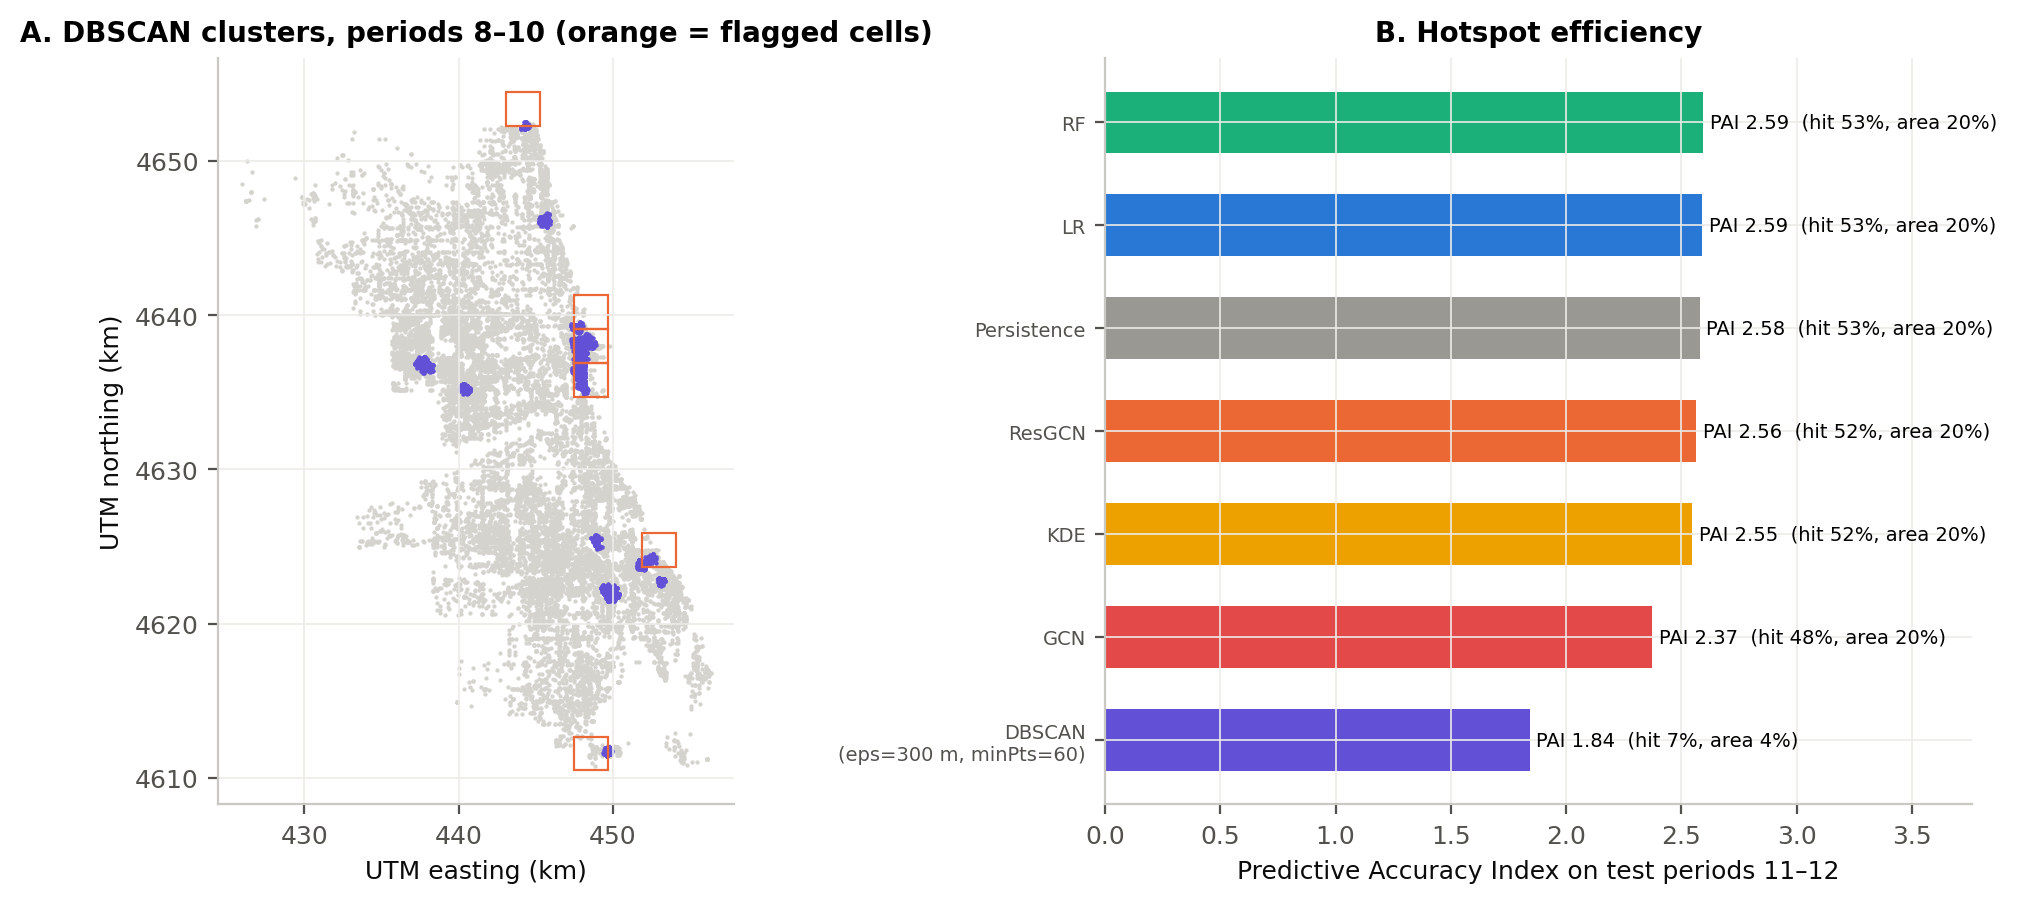
\includegraphics[width=\textwidth]{F12_dbscan_pai.png}
\caption{(A) DBSCAN clusters of victimisation incidents in periods 8--10 with flagged cells. (B) PAI on the test periods for DBSCAN zones and for the top-20\% cells of each ranking model.}
\label{fig:dbscan}
\end{figure}

It is unclear whether KDE itself would satisfy the unsupervised criterion in the way defined by the lecturer, and this is flagged for confirmation: KDE uses no labels, but here it served as a forecasting baseline and was scored against labels. To include a truly unsupervised element (LO3), DBSCAN \citep{ester1996} was performed on the location data of victimisation incidents. The values of $\varepsilon$ from the k-distance plot (30th neighbour) were used to create a grid ranging from 100 m to 300~m with minPts $\in\{30, 60, 100\}$; cells were marked as clusters when at least half of their incidents were clustered. Settings were chosen by PAI when fitted on periods 5--7 and validated on periods 9--10, re-fitted on periods 8--10 and tested on periods 11--12. The selected setting ($\varepsilon=300$~m, minPts $=60$) discovered 12 dense clusters (silhouette 0.63 among clustered points), marked 90\% of incidents as noise, identified six cells (3.8\% of the area) and captured 7.0\% of victimisation incidents from the test periods: a PAI value of 1.84 (Figure~\ref{fig:dbscan}). The supervised rankings with top-20\% cells led to PAI of 2.37--2.59, capturing around 53\% of incidents in 20\% of cells. A more liberal setting ($\varepsilon=300$~m, minPts $=30$) resulted in 36 flagged cells and PAI of 2.10 during the test period, but was not selected during the validation. The overlap between flagged cells in two distinct three-period windows was moderate (Jaccard 0.50).

These results highlight the strengths and limitations of the unsupervised approach. DBSCAN detects compact micro-hotspots within cells, which can be used as an informative layer to indicate \emph{within the flagged cell} where incidents cluster, but it is parameter dependent, and PAI gives high scores to very small areas; thus the validation-selected setting proved too conservative for area-level planning. The other density-based approach, KDE, achieved a much higher PAI (2.55). Thus, in this application, DBSCAN is a descriptive layer, not a decision-making tool.

\subsection{Computational Cost (E13)}
\begin{table}[H]
\centering\small
\caption{Measured computational cost (Apple M5 CPU; Phase~2; mean over seeds)}
\label{tab:cost}
\resizebox{\textwidth}{!}{\begin{tabular}{@{}lcccc@{}}
\toprule
Model & Trainable parameters & Fit time (s) & Inference for 314 cells (ms) & Best epoch\\
\midrule
LR & 24 & 0.004 & 0.2 & --\\
SVM (RBF) & support vectors & 0.003 & 1.7 & --\\
RF (300 trees) & -- & 0.21 & 25 & --\\
MLP & 3,330 & 0.19 & 0.2 & 160\\
GCN & 1,666 & 0.45 & 0.4 & 226\\
ResGCN & 6,660 & 0.77 & 0.5 & 278\\
KDE (per period, 18k points) & -- & -- & 38 & --\\
\bottomrule
\end{tabular}}
\end{table}
All models train in under one second on a laptop CPU and evaluate the entire city in milliseconds (Table~\ref{tab:cost}), and the full experiment set with 14 experiment groups and hundreds of model fits took under ten minutes, with peak memory use under 1~GB. Thus computational cost is not an issue at this level of analysis. It becomes an issue only at much higher resolutions or with daily retraining, where the GCN's block-diagonal snapshot graph scales linearly with periods $\times$ cells.


\subsection{Post-hoc Extensions: Preprocessing, Significance, Features, Counts and Effective Sample Size (E15--E19)}
\label{sec:posthoc}
These five analyses were added after the main test results became available to fill in any gaps identified while the report was evaluated using the rubric and Assessment~1. In order to avoid selection bias, each one of them uses validation data exclusively, without modifying the models selected in Sections~\ref{sec:p2res}--\ref{sec:p1res}. If one of them contradicts a previous statement, then that statement has been corrected.

\paragraph{Preprocessing (E15).} Table~\ref{tab:prepab} assesses how much each preprocessing step helps. Validation favours the full preprocessing pipeline for both LR models (validation AP 0.968 compared to 0.959 without; validation macro-F1 0.492 compared to 0.454), and the robust scaler performs the same. In test time frames, raw features provided a better AP for LR (0.993 compared to 0.983, with the penalty $C$ tuned to 0.01), an advantage too small for the bootstrap to resolve (about 0.01) and one that validation did not predict; using it would be selecting based on the test data, so it was not used. For Phase~1, the log transform and scaling clearly help (LR 0.498 vs 0.446 raw, MLP 0.477 vs 0.421). In the case of the GCN model, scaling matters, not the log transform (log transform 0.835, z-score 0.904, both 0.896), since the propagation technique relies heavily on the mixing of features across nodes, and unscaled counts dominate. Omitting the 17 low-volume cells from training did not benefit the logistic regression model (0.982) but hurt the GCN (0.781 versus 0.896) since the GCN requires every node to learn its neighbourhoods. The supported claim is thus a modest one, namely that preprocessing is essential to the neural network and Phase~1 models, retained on validation and data-quality grounds but does not explain the model rankings.
\begin{table}[H]
\centering\scriptsize
\caption{Preprocessing ablation (E15, post-hoc). LR is re-tuned per variant on validation; MLP, ResGCN and GCN (5 seeds) keep their E1/E3 hyperparameters}
\label{tab:prepab}
\resizebox{\textwidth}{!}{\begin{tabular}{@{}lccccccccc@{}}
\toprule
 & \multicolumn{5}{c}{Phase 2 AP} & \multicolumn{3}{c}{Phase 1 macro-F1}\\
\cmidrule(lr){2-6}\cmidrule(lr){7-9}
Variant & LR val. & LR test & MLP & ResGCN & GCN & LR val. & LR test & MLP\\
\midrule
log + z-score (main) & 0.968 & 0.983 & 0.980 & 0.975 & 0.896 & 0.492 & 0.498 & 0.477\\
raw & 0.959 & 0.993 & 0.983 & 0.961 & 0.875 & 0.454 & 0.446 & 0.421\\
z-score only & 0.960 & 0.982 & 0.977 & 0.974 & 0.904 & 0.473 & 0.476 & 0.462\\
log only & 0.958 & 0.985 & 0.979 & 0.969 & 0.835 & 0.486 & 0.482 & 0.410\\
log + robust scaling & 0.970 & 0.982 & 0.981 & 0.974 & 0.888 & 0.490 & 0.498 & 0.463\\
Drop 17 low-volume cells (train) & -- & 0.982 & 0.973 & 0.973 & 0.781 & -- & -- & --\\
\bottomrule
\end{tabular}}
\end{table}

\paragraph{Significance tests (E16).} Table~\ref{tab:perm} provides paired spatial-block permutation tests. The two model scores (percentile ranks within periods for Phase~2; predictions for Phase~1) are permuted within randomly selected $3\times3$-cell blocks and the AP or macro-F1 difference is recalculated 4,000 times, and $p$ is the proportion of permutations with a difference of at least the observed magnitude; Holm's correction is done within each family. In the one-year analysis three differences remain after correction: GCN is inferior to MLP ($p_\mathrm{Holm}=0.010$), residual GCN is superior to GCN (0.010), and GAT is inferior to MLP (0.032). None of the comparisons between LR, RF, MLP, SVM, ResGCN and persistence for victimisation is significant (lowest raw $p=0.18$), consistent with the bootstrap. For crime type, no difference remains after correction; LR vs. persistence has raw $p=0.077$ (Holm 0.53), which means that the improvement observed in Section~\ref{sec:p1res} is only tentative. The three-year columns tell the same story.

\begin{table}[H]
\centering\scriptsize
\caption{Paired spatial-block permutation tests (E16, post-hoc; 26 blocks, 4,000 permutations; Holm-adjusted within each task)}
\label{tab:perm}
\resizebox{\textwidth}{!}{\begin{tabular}{@{}lrrrrrr@{}}
\toprule
 & \multicolumn{3}{c}{One-year study} & \multicolumn{3}{c}{Three-year study}\\
\cmidrule(lr){2-4}\cmidrule(lr){5-7}
Comparison (difference in AP or macro-F1) & Diff. & $p$ & $p_\mathrm{Holm}$ & Diff. & $p$ & $p_\mathrm{Holm}$\\
\midrule
P2 AP: LR $-$ Persistence & +0.009 & 0.336 & 1.000 & +0.002 & 0.612 & 1.000\\
P2 AP: RF $-$ LR & +0.005 & 0.248 & 1.000 & +0.006 & 0.074 & 0.518\\
P2 AP: MLP $-$ LR & -0.001 & 0.797 & 1.000 & +0.003 & 0.543 & 1.000\\
P2 AP: SVM $-$ LR & -0.008 & 0.176 & 1.000 & -0.005 & 0.335 & 1.000\\
P2 AP: GCN $-$ MLP & -0.088 & 0.001 & 0.010 & -0.082 & 0.000 & 0.002\\
P2 AP: ResGCN $-$ MLP & -0.006 & 0.352 & 1.000 & +0.004 & 0.291 & 1.000\\
P2 AP: ResGCN $-$ GCN & +0.082 & 0.001 & 0.010 & +0.086 & 0.000 & 0.002\\
P2 AP: GAT $-$ MLP & -0.100 & 0.004 & 0.032 & -0.089 & 0.002 & 0.018\\
P2 AP: GAT $-$ GCN & -0.012 & 0.695 & 1.000 & -0.007 & 0.781 & 1.000\\
P2 AP: KDE $-$ Persistence & -0.002 & 0.747 & 1.000 & -0.013 & 0.293 & 1.000\\
P1 F1: LR $-$ Persistence & +0.095 & 0.076 & 0.527 & +0.043 & 0.138 & 0.589\\
P1 F1: GCN $-$ SVM & -0.019 & 0.419 & 1.000 & -0.052 & 0.059 & 0.357\\
P1 F1: GCN $-$ MLP & -0.032 & 0.202 & 1.000 & -0.040 & 0.118 & 0.589\\
P1 F1: LR $-$ GCN & +0.050 & 0.075 & 0.527 & +0.030 & 0.245 & 0.736\\
P1 F1: ResGCN $-$ GCN & +0.029 & 0.224 & 1.000 & +0.046 & 0.011 & 0.079\\
P1 F1: GAT $-$ GCN & +0.004 & 0.822 & 1.000 & +0.004 & 0.698 & 0.810\\
P1 F1: MLP $-$ LR & -0.018 & 0.559 & 1.000 & +0.010 & 0.405 & 0.810\\
\bottomrule
\end{tabular}}
\end{table}

\paragraph{Phase~1 feature extension (E17).} Eighteen additional history-only features were introduced (previous period and 6-period group ratios; dominant class features for final period and last three periods; dominance margin and mix entropy). The validation macro-F1 in Table \ref{tab:p1x} improved for RF (0.486 $\to$ 0.518) and ResGCN (0.490 $\to$ 0.514), was unchanged for MLP but declined for LR (0.492 $\to$ 0.466). Hence selection based on validation leads to extended features for RF, MLP and ResGCN but base features for LR. In the testing periods, the extended RF model performed better (0.461 $\to$ 0.518), whereas the extended MLP and ResGCN models performed poorly (0.477 $\to$ 0.434 and 0.462 $\to$ 0.433). Given about 300 test rows and eight model-feature combinations, the best result (extended-feature RF, 0.518) is optimistic. No feature set resolves the weakness of Phase~1.

\begin{table}[H]
\centering\small
\caption{Phase~1 feature extension (E17, post-hoc): macro-F1 on validation and test periods}
\label{tab:p1x}
\begin{tabular}{@{}lccccc@{}}
\toprule
 & \multicolumn{2}{c}{Base (23 features)} & \multicolumn{2}{c}{Extended (+18)} & Chosen on\\
Model & Validation & Test & Validation & Test & validation\\
\midrule
LR & 0.492 & 0.498 & 0.466 & 0.496 & base\\
RF & 0.486 & 0.461 & 0.518 & 0.518 & extended\\
MLP & 0.520 & $0.477\pm0.020$ & 0.521 & $0.434\pm0.032$ & extended\\
ResGCN & 0.490 & $0.462\pm0.026$ & 0.514 & $0.433\pm0.014$ & extended\\
\bottomrule
\end{tabular}
\end{table}

\paragraph{Tuned count models (E18).} Table~\ref{tab:count2} repeats the count comparison with neural models tuned on validation (24 configurations $\times$ 3 seeds each) and an extended Poisson $\alpha$ grid up to 100; the selected $\alpha=1$ is now interior. Tuning improved the MLP (MAE 6.27 vs 6.70) but it remains behind the three-period moving average (5.99) and the GLM (5.94). The tuned GCN is still markedly worse (MAE 11.47, $R^2=0.81$), the ResGCN is mid-table (7.24) and the GAT is worst (16.5, $R^2=0.55$). Missing tuning is therefore not the explanation for the GCN's count failure, and the smoothing explanation stands.

\begin{table}[H]
\centering\small
\caption{Tuned next-period victimisation count forecasts (E18, post-hoc; test periods, $n=314$)}
\label{tab:count2}
\begin{tabular}{@{}lcccc@{}}
\toprule
Model & MAE & RMSE & $R^2$ & Spearman $\rho$\\
\midrule
Persistence (last period) & 6.59 & 9.54 & 0.939 & 0.973\\
Persistence (3-period mean) & 5.99 & 8.62 & 0.950 & 0.979\\
Poisson GLM (tuned alpha) & 5.94 & 8.94 & 0.946 & 0.979\\
MLP (Poisson loss, tuned) & 6.27 & 9.37 & 0.941 & 0.977\\
GCN (Poisson loss, tuned) & 11.47 & 16.89 & 0.808 & 0.912\\
ResGCN (Poisson loss, tuned) & 7.24 & 10.92 & 0.920 & 0.972\\
GAT (Poisson loss, tuned) & 16.51 & 25.78 & 0.552 & 0.865\\
\bottomrule
\end{tabular}
\end{table}

\paragraph{Effective sample size and a weighted graph (E19).} Table~\ref{tab:neff} shows just how much independent information the test sets actually contain. Moran's $I$ statistic of log victimisation counts is around 0.5, and the lag-1 autocorrelation of the periods is around 0.96. Applying the heuristic $n_{\text{eff}} \approx n(1 - \rho)/(1 + \rho)$ to each of the dependencies, the 314 test rows of the main study correspond to only 47 effectively independent observations (roughly the number of cells), and the 948 rows from the three-year study to about 50, since the additional time periods are almost entirely redundant. It is an approximation rather than an accurate count, but it explains why differences of about 0.01 AP cannot be resolved and why the number of cells, not incidents or rows, limits the evidence. The table also provides the information on the centroid-based graph (distances between incident centroids from periods before the test window, according to the base paper): it is denser (mean degree 4.9-5.0) and its edge length varies (0.68-3.0~km), so the inverse distance weight does matter. Still, the GCN reached only 0.770 and the GAT 0.800 (one year), compared with 0.973 for the ResGCN, which means that the constant weight in the lattice did not cause the GCN's poor performance.

\begin{table}[H]
\centering\small
\caption{Effective sample size and centroid-graph check (E19, post-hoc)}
\label{tab:neff}
\begin{tabular}{@{}lcc@{}}
\toprule
Quantity & One-year study & Three-year study\\
\midrule
Cells (nodes) & 157 & 158\\
Test rows (cells $\times$ periods) & 314 & 948\\
Moran's $I$ of log victimisation counts (mean over test periods) & 0.540 & 0.519\\
Lag-1 correlation of log counts between periods & 0.964 & 0.965\\
Effective spatial sample $n(1-I)/(1+I)$ & 46.7 & 50.1\\
Effective independent periods per cell (floored at 1) & 1.0 & 1.0\\
Approximate effective sample size of the test set & 46.7 & 50.1\\
Centroid graph: undirected edges & 386 & 396\\
Centroid graph: mean degree & 4.92 & 5.01\\
GCN on centroid graph: AP / Phase 1 macro-F1 & 0.770 / 0.438 & 0.852 / 0.428\\
ResGCN on centroid graph: AP / Phase 1 macro-F1 & 0.973 / 0.469 & 0.962 / 0.464\\
GAT on centroid graph: AP / Phase 1 macro-F1 & 0.800 / 0.434 & 0.849 / 0.424\\
\bottomrule
\end{tabular}
\end{table}

\subsection{Three-Year Replication (E21)}
\label{sec:multi}

The primary experiment spans one year divided into two test periods. To establish whether the results of this study are an artefact of this time span, the entire comparison was reproduced over three years, from 24 August 2023 through 23 August 2026. The first two of these three years (509,905 records) are sourced from the same portal's \emph{Crimes -- 2001 to Present} database and concatenated with the one-year sample, which totals 739,180 records, 732,017 of which are cleaned. There are 158 occupied cells and 39 full 28-day periods in this concatenated sample. Period counts and victimisation, arrest and domestic shares show no discontinuity at the point of concatenation (period 26, covering it, contains 18,659 records, compared to 19,521 and 19,061 for adjacent periods). Protocol remains the same: features rely on past periods only; training data comprises periods 3--26 (up to 17~September 2025), validation periods 27--32 and test periods 33--38 (5~March to 19~August 2026); hyperparameters were tuned using validation only; the Phase~1 classes were derived again from training periods using the 5\% criterion and retained the classes of battery, criminal damage and theft (shares 33\%, 6\%, 52\%). Each model was executed with ten seeds.

Table~\ref{tab:multi} and Figure~\ref{fig:multi} confirm the replicability of the results. In Phase~2, RF (AP 0.965), the residual GCN (0.964), the MLP (0.958), LR (0.958), the SVM (0.952) and persistence (0.951) constitute one group where there is no statistically significant difference (LR minus persistence $+0.007$, 95\% CI $[-0.005, 0.016]$; RF minus LR $p=0.074$, Holm 0.52). The GCN (0.875) and GAT (0.870) are definitely poorer (GCN minus MLP $-0.084$, $p_\mathrm{Holm}=0.003$), so the quadrupling of the training periods from 6 to 24 did not close the graph gap. For Phase~1, RF (macro-F1 = 0.499) and SVM (0.492) take first place while GCN (0.443) ranks last among the learned models, and the benefit of LR over persistence decreases to only $+0.043$ ($p = 0.14$). The validation procedure would now select RF to proceed to Phase~2 (validation AP = 0.966 compared with 0.963 for LR), which is consistent with RF's test ranking and still within noise of LR.

\begin{table}[H]
\centering\small
\caption{Three-year replication (E21): test periods 33--38 ($n=948$ cell-periods, 192 high; Phase~1 support 899). Mean $\pm$ sd over 10 seeds; CI from the spatial-block bootstrap}
\label{tab:multi}
\begin{tabular}{@{}lccccc@{}}
\toprule
 & \multicolumn{3}{c}{Phase 2 (three years)} & Phase 1 & Phase 2 AP\\
Model & AP & AP 95\% CI & Top-20\% macro-F1 & macro-F1 & one-year study\\
\midrule
Persistence & 0.951 & [0.899, 0.979] & 0.935 & 0.427 & 0.973\\
KDE & 0.943 & [0.875, 0.978] & 0.925 & 0.467 & 0.970\\
LR & 0.958 & [0.904, 0.984] & 0.928 & 0.469 & 0.983\\
SVM & 0.952 & [0.889, 0.980] & 0.915 & 0.492 & 0.974\\
RF & $0.965\pm0.000$ & [0.923, 0.988] & $0.932\pm0.001$ & $0.499\pm0.004$ & 0.988\\
MLP & $0.958\pm0.002$ & [0.907, 0.985] & $0.931\pm0.003$ & $0.475\pm0.008$ & 0.980\\
GCN & $0.875\pm0.006$ & [0.780, 0.930] & $0.865\pm0.004$ & $0.443\pm0.006$ & 0.885\\
ResGCN & $0.964\pm0.001$ & [0.923, 0.987] & $0.929\pm0.003$ & $0.474\pm0.014$ & 0.975\\
GAT & $0.870\pm0.007$ & [0.788, 0.932] & $0.862\pm0.006$ & $0.442\pm0.009$ & 0.867\\
\bottomrule
\end{tabular}
\end{table}

\begin{figure}[H]
\centering
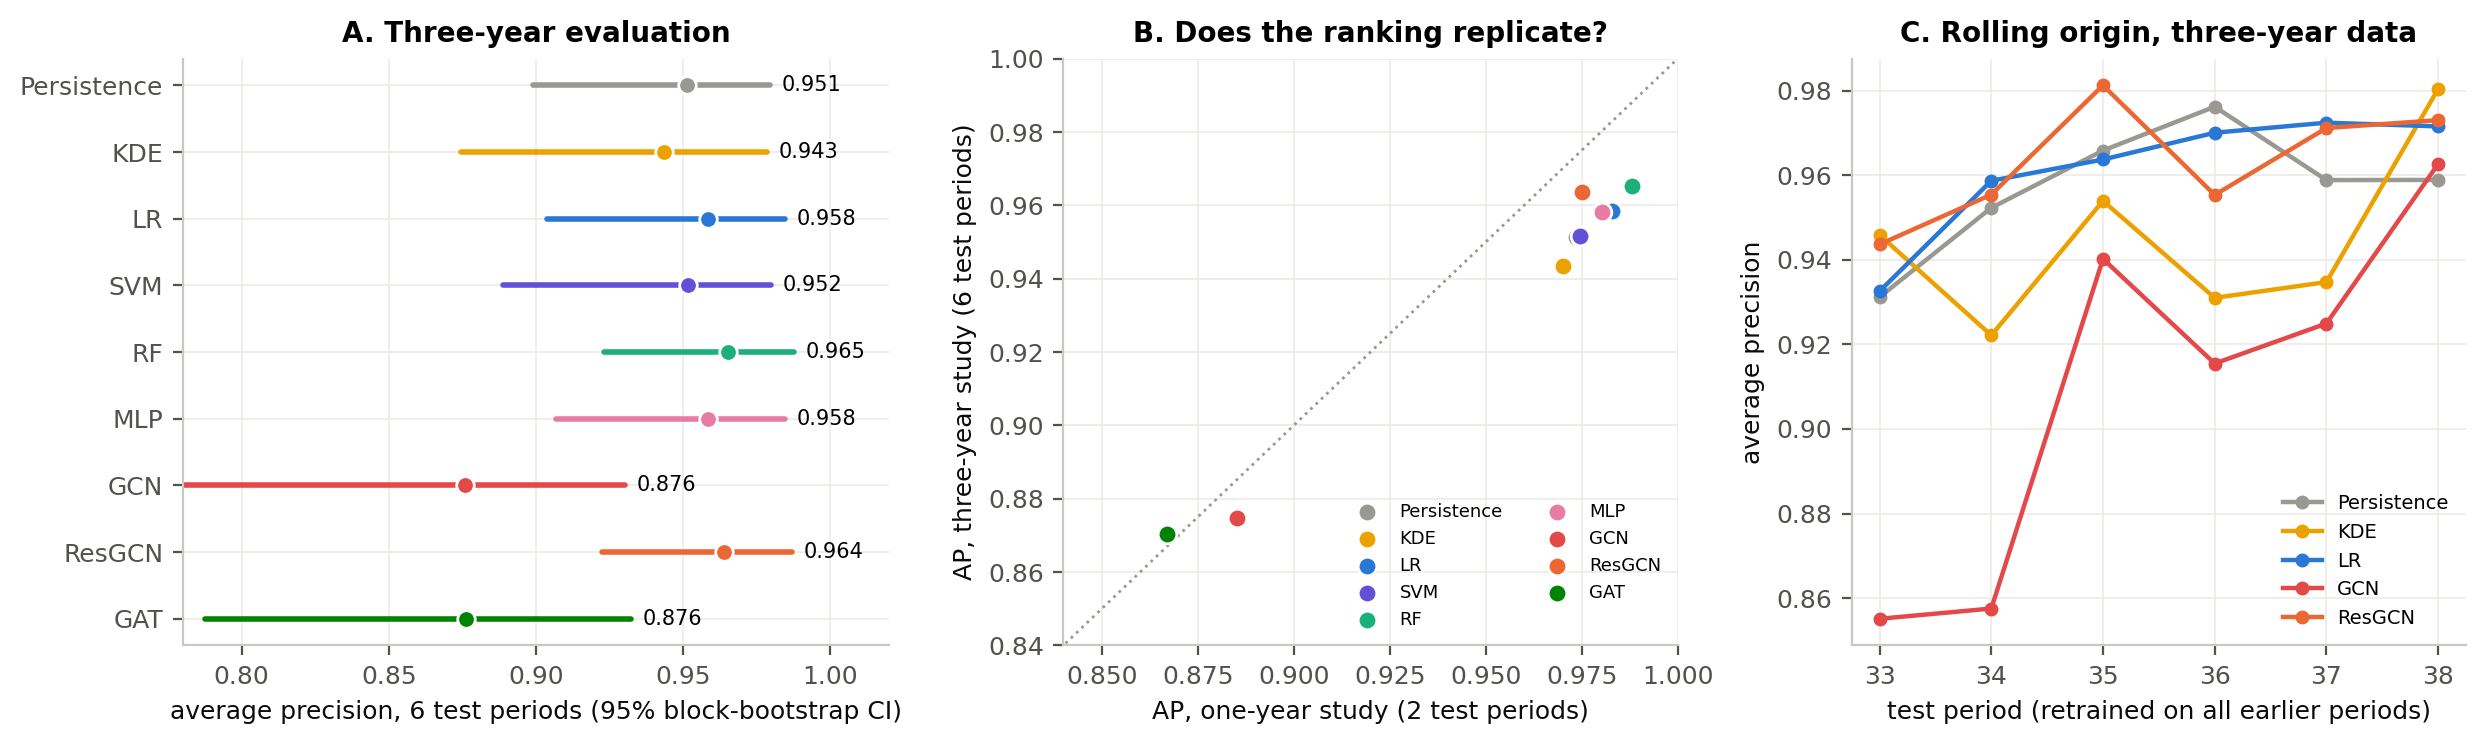
\includegraphics[width=\textwidth]{F15_multiyear.png}
\caption{Three-year replication. (A) AP with 95\% block-bootstrap intervals. (B) Model-by-model AP in the one-year and three-year studies, close to the diagonal for every model. (C) Rolling-origin AP over the test periods.}
\label{fig:multi}
\end{figure}

The long rolling origin includes the seasons from the second year (12 windows, test periods 15--37; retraining on all previous periods in each window). Table~\ref{tab:long} confirms that the GCN is worse than persistence, LR, and the residual GCN for all 12 windows, that LR is better than persistence for only 6 of 12 windows (mean AP 0.966 versus 0.968), and that the residual GCN equals persistence on average (0.968). For crime type, LR is better than persistence for 7 of 12 windows (mean macro-F1 0.494 versus 0.470), a difference that is consistent in sign but small. Holding out spatial blocks (E9) gives mean AP 0.897 for LR, 0.890 for the residual GCN, 0.886 for MLP, 0.884 for persistence and 0.742 for the GCN; the GCN is better only in block 0, which has only six high cell-periods out of 180, too few to interpret. In addition, the data for three years provide a second, independent check on the earlier findings about decision rules (Section 4.1.5), imbalance and the graph (Table~\ref{tab:neff}).

\begin{table}[H]
\centering\scriptsize
\caption{Long rolling origin on three-year data (E21): Phase~2 AP and Phase~1 macro-F1 by test period (start date); 5 seeds for the GCN and ResGCN}
\label{tab:long}
\resizebox{\textwidth}{!}{\begin{tabular}{@{}lccccccccc@{}}
\toprule
 & \multicolumn{5}{c}{Phase 2 AP} & \multicolumn{3}{c}{Phase 1 macro-F1}\\
\cmidrule(lr){2-6}\cmidrule(lr){7-9}
Test period & Persistence & KDE & LR & GCN & ResGCN & Persistence & LR & GCN\\
\midrule
15 (17 Oct 2024) & 0.987 & 0.979 & 0.972 & 0.919 & 0.974 & 0.490 & 0.516 & 0.478\\
17 (12 Dec 2024) & 0.989 & 0.977 & 0.992 & 0.951 & 0.988 & 0.538 & 0.487 & 0.458\\
19 (6 Feb 2025) & 0.981 & 0.949 & 0.973 & 0.896 & 0.962 & 0.468 & 0.515 & 0.479\\
21 (3 Apr 2025) & 0.969 & 0.971 & 0.951 & 0.894 & 0.969 & 0.510 & 0.504 & 0.457\\
23 (29 May 2025) & 0.960 & 0.963 & 0.954 & 0.903 & 0.950 & 0.480 & 0.531 & 0.517\\
25 (24 Jul 2025) & 0.988 & 0.956 & 0.994 & 0.950 & 0.991 & 0.446 & 0.414 & 0.381\\
27 (18 Sep 2025) & 0.954 & 0.970 & 0.957 & 0.898 & 0.950 & 0.389 & 0.527 & 0.505\\
29 (13 Nov 2025) & 0.972 & 0.949 & 0.981 & 0.926 & 0.982 & 0.527 & 0.516 & 0.482\\
31 (8 Jan 2026) & 0.960 & 0.935 & 0.950 & 0.898 & 0.957 & 0.415 & 0.461 & 0.438\\
33 (5 Mar 2026) & 0.931 & 0.946 & 0.933 & 0.855 & 0.944 & 0.506 & 0.500 & 0.453\\
35 (30 Apr 2026) & 0.966 & 0.954 & 0.964 & 0.940 & 0.981 & 0.479 & 0.489 & 0.388\\
37 (25 Jun 2026) & 0.959 & 0.935 & 0.972 & 0.925 & 0.971 & 0.386 & 0.463 & 0.454\\
\midrule
Mean & 0.968 & 0.957 & 0.966 & 0.913 & 0.968 & 0.470 & 0.494 & 0.457\\
\bottomrule
\end{tabular}}
\end{table}


\subsection{Extension Experiments: Label Definition, Error Disparity and Boosting (E22--E24)}
\label{sec:ext}
Three gaps that remained after the first full draft were closed with further post-hoc experiments. As with E15--E19, every choice in them used validation periods only, and none of them changed the selected models.

\paragraph{Narrower victimisation label (E22).} The main label counts 11 person-directed categories, which is broad (Appendix~\ref{app:dict}). E22 re-ran the Phase~2 comparison with a much narrower label: FBI index violent crime only (codes 01A homicide, 02 criminal sexual assault, 03 robbery, 04A aggravated assault and 04B aggravated battery), which covers 20,376 incidents (8.9\% of cleaned records, against 32.2\% for the main label). All features and the top-20\% label were rebuilt from this definition, and every model was re-tuned on periods 9--10. The two labels agree on 93.6\% of test cell-periods (Jaccard overlap of the high cells 0.75). Table~\ref{tab:violent} shows that the ranking of methods is unchanged: persistence (AP 0.943), LR (0.940), KDE (0.939), RF (0.932) and MLP (0.931) are again within about 0.01 of one another, the residual GCN is close behind (0.920), and the GCN is again last (0.874). All AP values are about 0.04 lower than for the broad label because rarer events give noisier counts. The conclusions in Section~\ref{sec:p2res} therefore do not depend on how broadly victimisation is defined.

\begin{table}[H]
\centering\small
\caption{Phase~2 test results with the narrower FBI index violent-crime label (E22; periods 11--12; 5 seeds for RF and neural models)}
\label{tab:violent}
\begin{tabular}{@{}lccccc@{}}
\toprule
Model & AP & ROC-AUC & Top-20\% precision & Top-20\% recall & Top-20\% macro-F1\\
\midrule
Persistence & 0.943 & 0.979 & 0.891 & 0.792 & 0.897\\
LR & 0.940 & 0.979 & 0.906 & 0.806 & 0.906\\
KDE & 0.939 & 0.978 & 0.906 & 0.806 & 0.906\\
RF & 0.932 & 0.979 & 0.900 & 0.800 & 0.902\\
MLP & 0.931 & 0.976 & 0.900 & 0.800 & 0.902\\
ResGCN & 0.920 & 0.973 & 0.891 & 0.792 & 0.897\\
GCN & 0.874 & 0.950 & 0.819 & 0.728 & 0.854\\
\bottomrule
\end{tabular}
\end{table}

\paragraph{Error disparity across areas (E23).} The earlier draft could not examine whether errors fall unevenly on poorer areas because no area-level socio-economic data had been joined. E23 joined the City of Chicago's community-area boundaries \citep{chicago2026ca} and its 2008--2012 census indicators \citep{chicago2026census} to the incidents (99.7\% of incidents fell inside a community area), gave each cell the incident-weighted mean of the hardship index of its community areas, and split the 156 matched cells into three equal hardship terciles (52 cells, 104 test cell-periods each). Test predictions from E2 and E3 were then compared across terciles, with 95\% intervals from a bootstrap that resamples cells (both test periods of a cell kept together). Table~\ref{tab:disparity} gives the results for the selected LR model, persistence and the GCN.

\begin{table}[H]
\centering\scriptsize
\caption{Test errors by community-area hardship tercile (E23; 104 test cell-periods per tercile; 95\% cell-bootstrap intervals in brackets)}
\label{tab:disparity}
\resizebox{\textwidth}{!}{\begin{tabular}{@{}llcccccc@{}}
\toprule
 & & \multicolumn{4}{c}{Phase~2 (top-20\% rule)} & \multicolumn{2}{c}{Phase~1}\\
\cmidrule(lr){3-6}\cmidrule(lr){7-8}
Model & Hardship tercile & Share high (true) & Share flagged & Recall & False-positive rate & Error rate & Macro-F1\\
\midrule
LR & Low & 0.125 & 0.125 & 0.85 [0.60, 1.00] & 0.022 [0.00, 0.06] & 0.49 & 0.34\\
 & Middle & 0.163 & 0.154 & 0.82 [0.58, 1.00] & 0.023 [0.00, 0.06] & 0.44 & 0.46\\
 & High & 0.346 & 0.337 & 0.97 [0.90, 1.00] & 0.000 [0.00, 0.00] & 0.24 & 0.56\\
\addlinespace
Persistence & Low & 0.125 & 0.106 & 0.69 [0.33, 0.92] & 0.022 [0.00, 0.06] & 0.39 & 0.40\\
 & Middle & 0.163 & 0.173 & 0.94 [0.78, 1.00] & 0.023 [0.00, 0.06] & 0.44 & 0.36\\
 & High & 0.346 & 0.337 & 0.92 [0.78, 1.00] & 0.029 [0.00, 0.07] & 0.36 & 0.32\\
\addlinespace
GCN & Low & 0.125 & 0.106 & 0.54 [0.15, 0.90] & 0.044 [0.00, 0.10] & 0.52 & 0.29\\
 & Middle & 0.163 & 0.144 & 0.53 [0.19, 0.83] & 0.069 [0.01, 0.13] & 0.48 & 0.44\\
 & High & 0.346 & 0.365 & 0.97 [0.91, 1.00] & 0.044 [0.00, 0.12] & 0.35 & 0.41\\
\bottomrule
\end{tabular}}
\end{table}

Three findings follow. First, the \emph{selection rate} is strongly unequal: LR flags 33.7\% of cell-periods in high-hardship areas against 12.5\% in low-hardship areas. This mirrors the recorded base rates almost exactly (34.6\% vs 12.5\%; Spearman correlation between hardship and test victimisation counts 0.37), so the model is not adding a disparity of its own, but it does mean that any use of the ranking directs attention mainly to poorer areas, which is the setting in which the stigma and feedback-loop risks of Section~\ref{sec:limits} apply. Second, \emph{error rates} for Phase~2 are close to parity: recall and false-positive rates for LR overlap across terciles, and the only visible gap (lower recall in low-hardship areas, 0.85 vs 0.97) has wide intervals because each tercile holds only 13--36 high cell-periods. Where there is a difference, high victimisation in better-off areas is the more likely to be missed, so these areas are not over-flagged. Third, Phase~1 is clearly \emph{less accurate in low-hardship areas} (LR error rate 0.49 vs 0.24; macro-F1 0.34 vs 0.56), because those cells have mixed, low-volume crime profiles (Figure~\ref{fig:errmap}B). This supports showing the crime-type forecast only as low-reliability context. The audit is limited: the census indicators date from 2008--2012, the comparison is between areas rather than population groups, labels are recorded incidents and so carry the same reporting bias, and the intervals are wide. It is therefore an error-disparity check, not a full group-fairness audit, and no fairness claim beyond it is made.

\paragraph{Gradient boosting (E24).} To check whether a stronger tabular learner would change the model choice, histogram gradient boosting (HGB; class-weighted, L2 penalty 1.0) was tuned on the validation periods over learning rate $\{0.03, 0.1\}$, depth $\{3, \text{unlimited}\}$ and $\{100, 300\}$ iterations. For Phase~2 its best validation AP (0.962) was below LR's (0.968), so the pre-stated rule would not select it; on test it reached AP 0.975 and top-20\% macro-F1 0.922 (5 seeds), between persistence and LR. For Phase~1 it reached macro-F1 0.463 (accuracy 0.584, $\kappa=0.37$; validation 0.526), below LR (0.498) and with the same weakness on \textsc{criminal damage} (F1 0.20). A more flexible learner therefore adds no skill here, which agrees with E17 and E19: the limit is the small number of independent cells, not model capacity.

\section{Discussion}
\paragraph{RQ1 (crime type).} No. Under a leakage-safe forecasting design the GCN (macro-F1 0.450) did not outperform the SVM (0.467), the MLP (0.482) or LR (0.498), and the GAT performed as well as the GCN (0.450). The pilot's apparent superiority (66.67\% vs 37.50\% accuracy) was due to a circular problem. Learned models have not been found to outperform persistence for crime type: LR's $+0.09$ macro-F1 (bootstrap CI $[0.006, 0.167]$) is borderline, and the permutation test yields $p=0.077$ (Holm 0.53). In the three-year replication the LR's advantage is reduced to $+0.04$ ($p=0.14$), RF (0.499) and the SVM (0.492) perform best, and the GCN (0.443) is again inferior to them; additional history variables (E17) improved RF (0.518) but not the neural models. RO2 is thus partially achieved.

\paragraph{RQ2 (victimisation).} Yes for history-based features; no for the graph. LR selects the top-20\% cells with precision 0.938 and recall 0.909 (macro-F1 0.951), comfortably meeting the RO3 threshold, and thus RO3 is fulfilled. The graph did not bring value in any of the three independent evaluations (graph vs MLP, neighbour features in LR, spatial block transfer). This is contrary to the prediction in Assessment~1 and \citet{zubair2025}, but is consistent with the theory, as the target here is the cell's own rank, the rankings are persistent with $\rho\approx0.97$, and symmetric normalisation removes precisely this type of information. It also confirms the high persistence baselines found in the hotspot literature \citep{chainey2008,bowers2004}.

\paragraph{RQ3 (signal versus chance).} The predictive skill is real and mainly attributable to persistence. All models are significantly better than the nulls (AP 0.21; macro-F1 0.44); the order of the models is stable in five test windows, three grid resolutions, a three-year replication study, and a 12-window rolling-origin analysis; and the GCN's deficit relative to the other models is significant ($p_\mathrm{Holm}=0.010$ one-year, 0.003 three-year). The \emph{increment} in learned models over persistence on victimisation (of around 0.01 AP) is within the margin of error (LR - persistence $p = 0.34$; LR beats persistence in only 6 out of 12 rolling windows). Since the test sets have only about 47-50 independent observations (E19), such a difference is not resolvable. The 4.4-fold difference in future victimisation between high- and low-risk cells in the proposal is a true description, but it is due to persistence of concentration rather than to model sophistication.


\paragraph{Model selection.} Using the pre-stated rule, \textbf{LR is chosen as the Phase~2 model} in the main analysis: the highest validation AP, tied with the best test AP (RF, $+0.006$ AP, CI includes zero), the best generalisation to new regions, 24 interpretable parameters, and millisecond training time. In the three-year replication, validation favours RF (0.966 vs 0.963), but still within noise, and persistence is a valid zero-cost alternative; LR is recommended on transparency grounds, while RF and ResGCN are monitored challengers. For Phase 1, the validation rule chose the MLP network; however, since LR is statistically equivalent and interpretable, the application displays only the crime type prediction of the LR as \emph{contextual information}. The main recommendation --- prefer an interpretable model over a more complex one, when the latter does not bring anything quantifiable --- is derived from the results rather than from the original preference for GCNs.



\paragraph{Unexpected findings.} Four findings were unexpected. (i)~LR reproduced the pilot result exactly. (ii)~GCN performance declined monotonically as graph size increased, making graph size a diagnostic for over-smoothing. Neither a GAT with learned attention nor a weighted centroid graph resolved the problem. (iii)~The effect of threshold tuning depended on the number of validation periods: it reduced performance with two periods and had a neutral effect with six. (iv)~Raw features gave LR a higher test AP than the main pipeline, although validation favoured the main pipeline. This discrepancy reinforces the need to base model selection on validation data. These findings informed the history-only rule, the residual GCN, the top-$k$ decision rule and the caution in Section~\ref{sec:posthoc}.

\paragraph{Objective attainment.} RO1 accomplished (counts reconcile; pipeline reproducible, including three-year extension); RO2 partly accomplished (forecasting done and evaluated, but no model performed well and the GCN did not outperform the SVM); RO3 accomplished (macro-F1 0.951 $>$ 0.70, though the criterion turned out to be weak); RO4 accomplished (seeds, block bootstrap, permutations, rolling origin, spatial blocks, ablation studies, three-year replication); RO5 accomplished in terms of design and prototype of the batch job, API and dashboard, but not as a deployed system.

\paragraph{Issues and challenges encountered.} Table~\ref{tab:issues} records the practical challenges met during the project, how each was handled and what remains open.

\begin{table}[H]
\centering\scriptsize\renewcommand{\arraystretch}{0.9}
\caption{Issues and challenges encountered, responses and status}
\label{tab:issues}
\begin{tabularx}{\textwidth}{@{}L{2.5cm} Y Y L{1.7cm}@{}}
\toprule
Issue & How it was detected & Response in the solution & Status\\
\midrule
Circular Phase 1 label & Arg-max of pilot features reproduced the label for all 157 cells (E0) & History-only features; forecasting reframing; leakage rule documented & Resolved\\
Single random split, 5 positive test cells & Pilot recall moved 20 points per cell; LR matched pilot perfectly & Chronological 314-row test; rolling origin; block bootstrap & Resolved\\
Counts did not reconcile & 228,635 expected vs 228,595 observed & Stage-wise log found 40 missing coordinates & Resolved\\
String-valued arrest/domestic counts & Saved pilot CSV had ``NNYN\ldots'' values & Flags converted to 0/1 before aggregation & Resolved\\
Constant edge weights & All edges 2.2~km; weights unused by pilot & Weighted vs unweighted and larger graphs tested (E5) & Resolved (documented)\\
GCN over-smoothing & GCN below MLP; worse as degree grows & ResGCN with self path; graph ablations & Partly resolved (no graph gain)\\
Rare and singleton classes & One-cell SEX OFFENSE class; 27-row criminal-damage class & Training-only grouping rule; class weights; macro-F1 & Partly resolved (weak minority F1)\\
Threshold instability & Tuned thresholds hurt test F1 with 2 validation periods, neutral with 6 (E4, E21) & Prevalence-matched top-$k$ decision rule; tuning only with $\geq6$ validation periods & Resolved\\
Hyperparameter tension in proposal & Fixed paper settings vs promised search & Validation-only grid, 3 seeds & Resolved\\
Spatial dependence in evaluation & Neighbouring errors correlated; $n_\mathrm{eff}\approx47$--50 (E19) & Spatial-block bootstrap, permutation tests, block CV, three-year replication & Partly resolved (effective $n$ stays small)\\
DBSCAN parameter sensitivity & PAI favoured tiny areas & Used as descriptive layer only & Unresolved for decisions\\
Reporting and enforcement bias & Recorded data reflect policing & Framing, governance and audit design (\S\ref{sec:app}) & Unresolved (needs external data)\\
Single-year evidence & One-year extract, two test periods & Three-year replication and 12-window rolling origin (E21) & Resolved for Chicago; other cities untested\\
Preprocessing benefit asserted, not measured & Rubric check of Section~\ref{sec:transform} & Ablation (E15): modest, model-dependent effect; claim narrowed & Resolved\\
Statements about the base paper and references & Re-reading the paper; online source check & Graph-statistics claim corrected; all 27 references checked against an external source & Resolved (all DOIs confirmed through Crossref or publisher pages)\\
Learned neighbourhoods and tuning as alternative explanations & Reviewer-style objections & GAT, centroid graph, tuned count models (E18--E19) & Resolved (graph still no gain)\\
Broad victimisation label & 11 categories, 32\% of records, very different offence types & Re-run with FBI index violent crime only (E22); ranking unchanged & Resolved\\
Unequal impact across areas & Flags concentrate where hardship is high & Error-disparity audit by hardship tercile (E23); low-reliability display for Phase~1; governance & Partly resolved (selection rate follows recorded base rates)\\
Limited model capacity as an explanation & Could a stronger learner fix Phase~1? & Gradient boosting tuned on validation (E24): no gain & Resolved (limit is data, not capacity)\\
\bottomrule
\end{tabularx}
\end{table}

\section{Limitations}
\label{sec:limits}
\paragraph{Data coverage and label construction.} The main study uses one year of data from a rolling extract, which, according to CPD, is preliminary and not comparable over time; later reclassifications made after download are not reflected. The three-year replication includes two downloads spaced two months apart, and while there is no visible break in either counts or shares at the point where the two data sets are joined, minor differences in classification of data cannot be ruled out. The main test window covers a single summer (28 June to 22 August 2026), while the replication consists of six additional testing periods and a 12-period rolling origin that includes the summers of 2024--26. Victimisation rate uses the number of incidents committed against individuals and not victims, and the data has not been population or footfall adjusted, so locations with many people during the day, such as the Loop, would score highly because of visitor numbers rather than risk to residents. Homicides are counted per victim in the source, which is slightly inconsistent with the other categories.


\paragraph{Small effective sample and spatial autocorrelation.} Although there are 228,595 events (732,017 in the replication), there are only 157--158 cells, and cell-periods are highly auto-correlated in time ($\rho\approx0.96$) and space (Moran's $I\approx0.5$). The heuristic effective sample size is around 47 for the test and 50 for the replication (E19), so additional periods do not contribute much new information. Dependence-aware intervals are wider than naïve intervals, and differences of roughly 0.01 AP are not resolvable. Independent information would require more cells, that is, more cities.

\paragraph{Temporal leakage and reproducibility.} While the history-only constraint avoids feature leakage, the Phase~1 class categorisation and victimisation categories list were defined by the analyst with knowledge of the full category table (although only the training periods determined which categories were retained). The experiments E15--E19 and E22--E24 were planned after the main test outcomes were known; they employ validation data for all choices and do not alter the main findings, but are post-hoc and should be treated as such with respect to the test results. Repeating experiments E1, E3 and E10 with modified code yielded the same results as before while repeating experiments E4, E11 and E12 resulted in byte-identical outputs; neural nets were trained on CPU with the same seed every time, but are not necessarily bitwise repeatable across hardware.


\paragraph{Unmeasured confounding and features.} Only crime-record features were used; features such as land use, population, places of interest, weather and events were not used; hence the model cannot differentiate between where the harm occurs and where it was reported. Feature importance is an indicator of predictive relationship and not causality.

\paragraph{Reporting bias, feedback loops and fairness.} Recorded incidents reflect reporting practices and enforcement effort as well as actual incidents \citep{lum2016,richardson2019}. Since the chosen model is based primarily on past counts, any implementation that increases enforcement efforts to flagged cells may increase future counts in those cells and ensure that they remain in the top rankings \citep{ensign2018}. No demographic variables were used as model inputs. An area-level error-disparity audit (E23, Section~\ref{sec:ext}) found that Phase~2 recall and false-positive rates are close across hardship terciles, but that the model flags high-hardship areas about 2.7 times as often as low-hardship ones, following the recorded base rates. Because the census indicators are dated and the comparison is between areas rather than population groups, this is not a full group-fairness audit and no fairness claim beyond it is made. Area-level outputs reduce privacy risk relative to person-level prediction, but labelling areas as ``high victimisation'' may still cause stigmatisation of the population.

\paragraph{External validity.} Results are specific to Chicago, 2023--26, a 2.2~km grid and 28-day periods. Transfer to New Zealand cities is untested.

\section{Application Conversion}
\label{sec:app}
Figure~\ref{fig:arch} shows the proposed architecture of the application.

This section describes how the chosen solution would be converted into a working application. Nothing here has been deployed. The batch scoring job, read-only API and dashboard have been implemented as a prototype (Folder \texttt{Assessment2/app}) and validated automatically (Table~\ref{tab:proto}); the rest are design only.

\paragraph{Users and workflow.} The main users are community safety or crime analysts who develop a 28-day prevention plan such as assigning outreach workers, environmental design reviews, or victim support visits. The workflow includes the following steps: (1)~Once each period ends, the system refreshes the data and ranks all cells; (2)~The analyst sees a list and map of the top 32 cells, along with their history and uncertainty; (3)~The analyst logs a decision (include, exclude, or flag for review) and an explanation; and (4)~After the next period ends, results are compared to predictions. The model never allocates resources automatically.

\paragraph{Views.} \emph{Map view}: cells coloured based on forecast rank category (top 10\%, 10\% to 20\%, others), with the DBSCAN micro-hotspot layer and the KDE surface as optional overlays. \emph{Ranked list}: Rank, cell ID and name, forecast score, change in rank compared to previous period, and a time series for the four most recent periods of victimisation counts. \emph{Cell detail}: Sparkline of 13-period history, top three features as indicated by LR coefficients (Table~\ref{tab:imp}), crime type forecast as ``low reliability'' (macro-F1 $\approx0.5$), and an evidence panel specifying model version, training periods, and testing performance. \emph{Uncertainty}: rank intervals from bootstrapping the training cells, and a tag for cells within two ranks of the cut-off, since the 10 test cell-periods within two ranks of the cut-off (3\% of rows) contain 4 of the 10 errors (40\% error rate vs 2\% elsewhere; E20, Figure~\ref{fig:errmap}A).

\paragraph{API.} The read-only REST service exposes forecasts to the dashboard and other approved systems. The response below is illustrative (the values are not real forecasts).
\begin{small}
\begin{verbatim}
GET /v1/forecasts?period=2026-08-23&top_k=32
200 OK
{ "period_start": "2026-08-23", "period_days": 28,
  "model": {"name": "lr-victimisation", "version": "1.0.0",
            "feature_schema": "fs-2026.1", "grid": "utm16n-2200m-v1",
            "trained_on_periods": "2025-11-16..2026-07-25"},
  "cells": [ {"grid_id": "12_7", "rank": 1, "score": 0.997,
              "band": "top10", "rank_interval": [1, 3],
              "history_victim_counts": [181, 177, 191],
              "near_cutoff": false,
              "top_factors": ["long-run victimisation mean",
                              "recent total incidents"]} ],
  "disclaimer": "Area-level recorded-incident forecast; not a
                 measure of individual risk." }
\end{verbatim}
\end{small}
Input validation refuses periods that have not yet closed, unknown grid versions and requests for individual-level data. All responses are logged.

\paragraph{Preprocessing parity and versioning.} The cleaning, projection, gridding, and feature code in this work are provided as one versioned library that is imported for both training and scoring, thus ensuring that the same set of transformations (boundary filter, EPSG:26916 projection, grid origin, log transform, scaler) are applied at inference time. The model registry contains the model, the fitted scaler, the feature schema hash, the grid and graph version, training periods, and test metrics all in one artifact; a scoring job refuses to run if any hashes differ.

\paragraph{Batch versus online inference.} Forecasts get updated only upon the completion of a period, hence batch prediction for every 28 days, and also an optional ``period-to-date'' weekly prediction update are sufficient, so online inference is unnecessary. The measured cost (Table~\ref{tab:cost}) is in milliseconds for city-wide prediction runs and under one second per retraining on a laptop processor. Thus the model can be run on a small virtual machine and an available analytics server. If no existing server is available, the smallest general-purpose cloud machine is more than enough: AWS's public price list (published 29 October 2026) gives on-demand Linux rates of US\$0.0264 per hour for a \texttt{t3.small} (2 vCPU, 2~GiB) and US\$0.0528 per hour for a \texttt{t3.medium} (4~GiB) in the Sydney region \citep{aws2026}. Table~\ref{tab:runcost} turns these into monthly estimates. Staff effort, not computing, is therefore the main cost (Table~\ref{tab:feas}).

\begin{table}[H]
\centering\small
\caption{Running-cost estimate (assumptions: AWS Sydney on-demand Linux prices of 29 October 2026; 730 hours per month; storage, data transfer and tax excluded; prices change and should be re-checked before purchase)}
\label{tab:runcost}
\begin{tabularx}{\textwidth}{@{}Yccc@{}}
\toprule
Option & Hourly price (US\$) & Hours per month & Monthly cost (US\$)\\
\midrule
\texttt{t3.small}, always on (API + dashboard + batch job) & 0.0264 & 730 & 19.27\\
\texttt{t3.medium}, always on (headroom for retraining challengers) & 0.0528 & 730 & 38.54\\
\texttt{t3.small}, batch job only (13 runs a year, 1 hour each) & 0.0264 & $\approx$1.1 & 0.03\\
\bottomrule
\end{tabularx}
\end{table}

\paragraph{Graph models, new nodes and coverage changes.} The ResGCN candidate uses a static and versioned grid graph. A cell that is newly created by an annexation or geocoding change will have no previous history, hence it gets a ``cold start'' flag, and the LR champion, which needs no neighbours, scores it using the available lags. The grid graph gets recreated, and the GCN gets trained only during the next scheduled release period. The change in the grid size or origin will cause a new graph version and requires full re-evaluation, because all features and labels change.

\paragraph{Monitoring, delayed labels and retraining.} The labels are received 28 days after each forecast (plus the seven-day delay of the portal). For each closed period, the system calculates the AP, top-$k$ precision, and recall with respect to the actual counts, and compares them with the acceptance bands based on the rolling origin analysis (AP $\geq 0.94$, top-$k$ precision $\geq 0.85$). The feature drift is assessed via population stability indices for the main count features, and label drift via the percentage of cells switching bands. The model is retrained every third period or when an alert is triggered; the retrained challenger becomes the new champion if it equals or outperforms the current one in the last two closed periods. Every release keeps the previous version available for one-click rollback.

\paragraph{Security, access and audit.} The access is limited to designated analysts via the single sign-on capability of the organization with role-based privileges (viewer, analyst, administrator). The application keeps only area-based aggregations, while the incidents are stored in the source system. All queries, exports, and analyst overrides are recorded in an append-only audit log, which is used in the bias assessment below.

\paragraph{Responsible-use safeguards.} Interface labels describe outputs as forecasts of recorded incidents, neighbourhood names omitted from exports by default, and a required written reason for any action targeting a flagged neighbourhood. A quarterly check is done to see if forecasted bands align with independent metrics (e.g., hospital assault presentations or victimisation survey, when applicable) in order to see if there is any feedback loop \citep{ensign2018}, and any enforcement-oriented use is paired with non-enforcement interventions. The use of a census-based group-fairness audit is a prerequisite for broader adoption.

\paragraph{Built and tested prototype (E20).} The prototype implements a batch job that fits the model and scores every cell for each period using only historical data. It also produces bootstrap rank intervals and explains the top factors behind the predictions. The prototype includes a read-only JSON API that follows the response schema above, API-key roles, input validation, an append-only audit log and an HTML dashboard with a ranked list and a map. At start-up, it rejects any prediction store whose feature-schema hash differs from the one expected by the code. The serving layer uses only the Python standard library.
All 20 automated tests summarised in Table~\ref{tab:proto} passed. The parity test confirmed that the forecasts served for the two test periods matched the offline E2 results exactly, with an AP of 0.983, a top-20\% precision of 0.938 and a recall of 0.909. This agreement shows that the preprocessing used to serve forecasts matches the preprocessing used in training. The median latency for 600 mixed requests was 0.40~ms (95th percentile 0.50~ms) on the local machine, so it gives no information on network or load conditions; the prediction store size is 423~kB. The prototype has also demonstrated that the near-cut-off flag is a useful feature, since 10 of the 314 test cell-periods carry it and 4 of those 10 are misclassified, against 6 errors among the other 304. Not implemented: online inference, authentication beyond API keys, automated retraining, drift detectors, fairness review.


\begin{table}[H]
\centering\small
\caption{Prototype tests (E20): 20 of 20 passed}
\label{tab:proto}
\begin{tabularx}{\textwidth}{@{}L{3.1cm} c Y@{}}
\toprule
Test group & Tests & What is checked\\
\midrule
Access control & 4 & Missing and wrong keys rejected (401); viewer blocked from cell history (403); analyst allowed\\
Input validation & 6 & Unknown cell (404); non-integer, unknown period, $k=0$, $k=1000$ and unknown grid version (400)\\
Response contract & 5 & Health endpoint; unclosed period flagged; disclaimer, model and schema version present; City of Chicago data-modification notice present; ranks 1--32 without gaps\\
Serving parity & 2 & Served AP equals offline AP; served top-20\% precision and recall equal offline\\
Safeguards & 3 & Dashboard renders with disclaimer; mismatched schema refused at start-up; every request in the audit log\\
\bottomrule
\end{tabularx}
\end{table}

\begin{figure}[H]
\centering
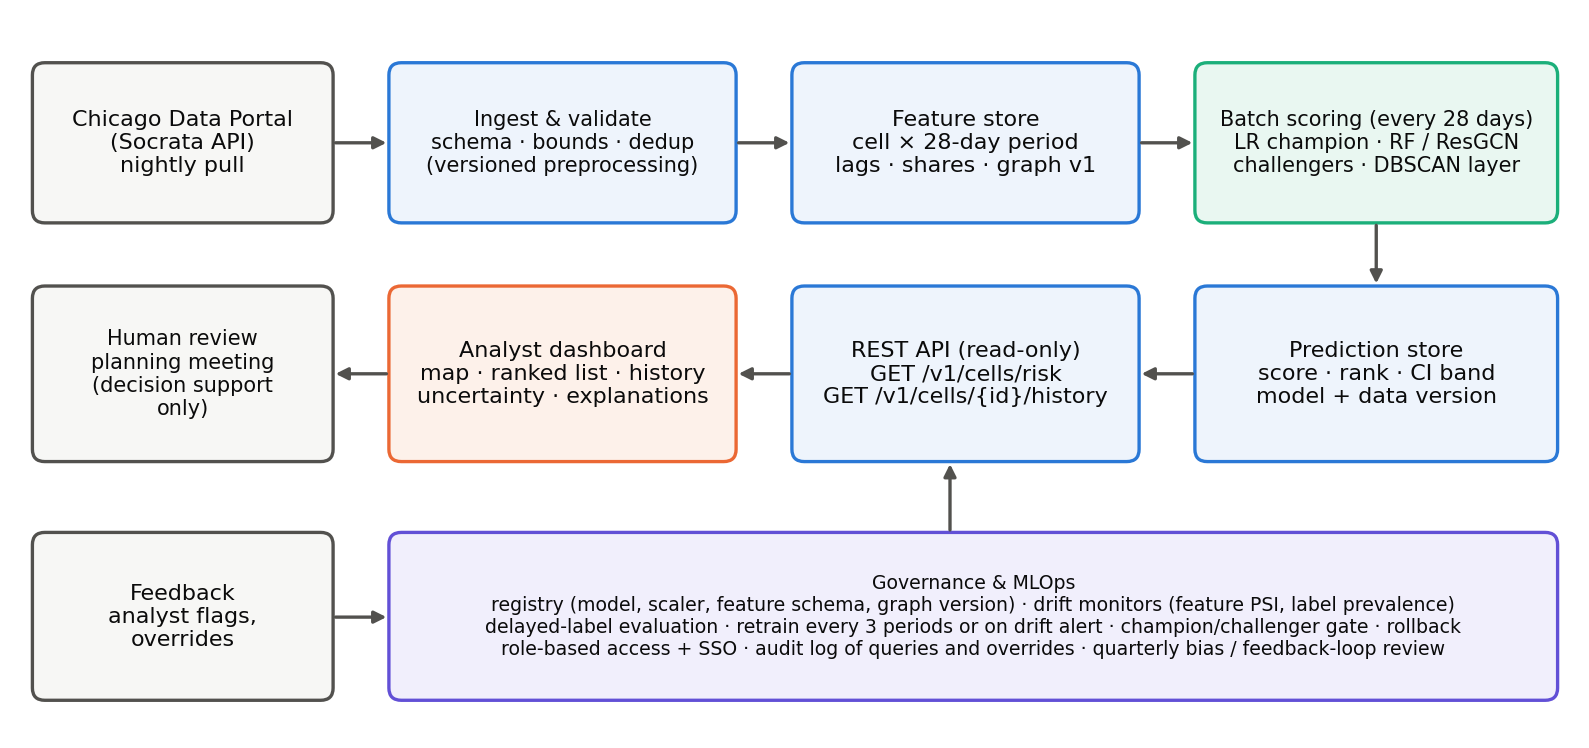
\includegraphics[width=\textwidth]{F14_architecture.png}
\caption{Proposed application architecture (design, not deployed).}
\label{fig:arch}
\end{figure}

\begin{table}[H]
\centering\small
\caption{Staged implementation plan and feasibility (assumptions: one analyst-developer; existing server; open data)}
\label{tab:feas}
\begin{tabularx}{\textwidth}{@{}L{2.4cm} Y L{2.6cm} L{3.6cm}@{}}
\toprule
Stage & Deliverable & Effort (estimate) & Acceptance criterion\\
\midrule
0. Built here & Reproducible pipeline, models, evaluation, figures; prototype batch job, API and dashboard & Completed & Counts reconcile; test AP 0.983; 20 of 20 API tests pass; served metrics equal offline\\
1. Shadow mode & Nightly ingest, 28-day batch scoring, internal dashboard; no operational use & 3--4 weeks & 3 consecutive periods with AP $\geq0.94$ and no pipeline failures\\
2. Pilot with analysts & Ranked list, cell detail, override logging, monitoring & 4--6 weeks & Analysts rate usefulness; overrides reviewed; no drift alerts unexplained\\
3. Governed release & SSO/RBAC, registry, rollback, quarterly bias review & 4 weeks & Governance sign-off; E23 disparity audit repeated on current census data\\
4. Extensions & Covariates (land use, population), multi-year data, ResGCN challenger & Ongoing & Challenger beats champion on two closed periods\\
\bottomrule
\end{tabularx}
\end{table}

\paragraph{Innovation and problem-solving.} The design responds to specific issues identified in this study. The top-$k$ rule addresses the threshold instability observed in E4, and the near-cut-off flag targets the errors shown in Figure~\ref{fig:errmap}. The cold-start process addresses the GCN's dependence on a fixed graph, while preprocessing parity addresses the pilot's file-level defects. Delayed-label monitoring and a champion--challenger gate allow more complex models to remain candidates and make them available to users only once they demonstrate added value.

\section{Chapter Summary}
Forecasts tested chronologically under a leakage-safe protocol show that recorded victimisation hotspots are highly predictable (AP 0.983, macro-F1 0.951), with persistence accounting for most of the predictive performance. The pilot-style GCN underperformed because symmetric normalisation over-smoothed the cell-level signal. The residual GCN addressed this problem, but the evaluation found no added benefit from information about neighbouring cells. Forecasting the dominant crime type remains challenging. The findings hold under a narrower violent-crime label and with a gradient-boosting learner, and the area-level disparity audit shows similar error rates but unequal selection rates across hardship terciles. The selected logistic regression model is computationally inexpensive, easy to interpret and robust across periods and areas. The application design incorporates versioning, monitoring and governance to support responsible use of the model as a decision-support tool.
% =====================================================================
\chapter{Conclusion}
\label{ch:conc}
The aim of this project was to forecast where recorded crime and recorded victimisation will concentrate in Chicago using 2.2~km cells so as to inform prevention planning. In Assessment~1, spatial GCNs were used to solve two tasks, and encouraging results from the pilot experiment were presented. In this study, the audit of the pilot showed that the Phase~1 task was circular; that the Phase~2 evaluation used only five positive test cells; that LR and persistence were able to match or beat the pilot GCN result. A leakage-safe forecasting pipeline was then developed: 228,595 reconciled events, 157 cells, thirteen 28-day periods, 23 history-only features, ten model families with the same tuning budget, chronological testing, ten random seeds, and spatial-block uncertainty estimates.

The confirmed results are clear. Cells that will fall into the top 20\% for recorded victimisation in the next period are predicted with high precision (LR: AP 0.983, macro-F1 0.951, precision 0.938, recall 0.909), much higher than the pre-specified benchmark, but a recency-weighted persistence method is almost equally accurate (AP 0.973), and the permutation tests find no significant differences between LR, RF, MLP, SVM, residual GCN, and persistence. A three-year replication using six test windows yielded similar results (RF 0.965, residual GCN 0.964, LR 0.958, persistence 0.951; GCN 0.875, GAT 0.870), and in a 12 window rolling origin LR outperformed persistence only 6 times. The pilot-style GCN under-performed (AP 0.885) because symmetric normalisation on the rook lattice gives each cell only about a fifth of the weight on its own history; graph ablations confirmed that performance falls as neighbourhoods widen or layers are added. The residual GCN, derived from this analysis, recovers the loss (AP 0.975) but does not benefit from neighbouring cells, and neither does a graph attention network, a weighted centroid graph, hand-crafted spatial-lag features or spatial-block transfer. The dominant crime type in the next period is much harder to predict (highest macro F1 about 0.50). Improvements in LR over persistence are suggestive but not significant (permutation $p=0.077$) while additional features helped RF but not the neural networks. Clusters generated by DBSCAN (unsupervised) are useful for describing micro-hotspots but less effective than ranked cells for area planning (PAI 1.84 vs 2.59). The same ranking of methods held with a much narrower violent-crime label (E22), gradient boosting added no skill (E24), and an area-level audit found similar Phase~2 error rates across hardship terciles but flags concentrated where recorded victimisation and hardship are highest (E23).

The chosen solution is thus a transparent, regularised logistic regression ranking model with persistence and KDE as reference layers, RF and ResGCN as monitored challengers, and a governed application that provides ranked, uncertain, area-level forecasts to analysts. A prototype for the batch job, API, and dashboard was constructed and tested (20 out of 20 tests; forecasts served by the prototype match the offline metrics exactly). Objectives RO1, RO3, and RO4 were reached, RO2 was partly reached, and RO5 was reached as a design with a tested prototype. These problems included label leakage, a small pilot test set, irreconcilable counts, malformed flag features, constant graph weights, over-smoothing, unstable decision thresholds and some overly-strong claims in the literature review in the proposal---and were all identified through explicit checks and mitigated (Table~\ref{tab:issues}). The reporting bias and feedback loop problem are still open, and have governance solutions only.


The study provides public-sector analysts with an inexpensive, interpretable ranking validated on held-out data. It also offers evidence about when a more complex model may offer too little benefit to justify its cost. The findings support short-horizon, area-level forecasting of \emph{recorded} incidents in Chicago using data from 2023--26. Performance in other cities, at finer spatial scales and in operational use remains untested. In practice, actions taken in response to forecasts may change the data recorded later.


\paragraph{Future work.} Each item follows from a specific finding:
\begin{enumerate}
\item \textbf{More cities and longer histories.} The three-year replication shows that the findings are stable over time in Chicago, but differences of about 0.01 AP still cannot be resolved because the number of cells, not periods, limits the evidence (E19); other cities would add independent cells and test transfer.
\item \textbf{Non-crime covariates} (population, land use, transit, points of interest), as \citet{zhang2020} found useful, to separate where harm occurs from where it is recorded and to allow population-adjusted rates.
\item \textbf{Graph models that learn the neighbourhood}---attention-based or learned-adjacency GNNs, and spatio-temporal models such as those of \citet{han2020}---evaluated against the strong persistence and LR baselines established here.
\item \textbf{Count-based ranking} with properly tuned Poisson or negative-binomial models, since counts carry more information than a binary top-20\% label.
\item \textbf{A fuller fairness and feedback audit} that extends the area-level check of E23 with current census-tract data and independent victimisation measures (surveys, hospital data) before any operational use.
\item \textbf{A shadow-mode deployment} (Stage~1 of Table~\ref{tab:feas}) to measure performance on genuinely future data and analysts' use of the outputs.
\end{enumerate}

% =====================================================================
\clearpage
\phantomsection
\addcontentsline{toc}{chapter}{References}
\bibliographystyle{apacite}
\bibliography{references}

% =====================================================================
\appendix
\renewcommand{\thesection}{\thechapter.\arabic{section}}

\chapter{Data Dictionary}
\label{app:dict}
\begin{table}[H]
\centering\scriptsize
\caption{Model features (computed per cell for target period $t$ from periods $<t$ only)}
\label{tab:dict}
\begin{tabularx}{\textwidth}{@{}L{4.2cm} Y L{2.6cm}@{}}
\toprule
Feature & Definition & Transform\\
\midrule
VICTIM\_L1, \_L2, \_L3 & Victimisation-related incidents in periods $t-1$, $t-2$, $t-3$ & $\log(1+x)$, z-score\\
TOTAL\_L1, \_L2, \_L3 & All incidents in periods $t-1$, $t-2$, $t-3$ & $\log(1+x)$, z-score\\
VICTIM\_MEAN\_ALL & Mean victimisation incidents per period over periods $0,\dots,t-1$ & $\log(1+x)$, z-score\\
TOTAL\_MEAN\_ALL & Mean incidents per period over periods $0,\dots,t-1$ & $\log(1+x)$, z-score\\
VICTIM\_SHARE & Victimisation share of all incidents in periods $<t$ & z-score\\
DOMESTIC\_SHARE & Share flagged domestic in periods $<t$ & z-score\\
ARREST\_SHARE & Share with arrest in periods $<t$ & z-score\\
NIGHT\_SHARE & Share occurring 20:00--05:59 in periods $<t$ & z-score\\
VICTIM\_TREND & VICTIM\_L1 $-$ VICTIM\_L3 & signed log, z-score\\
SHARE3\_\{category\} (8) & Share of incidents in periods $t-3..t-1$ that are theft, battery, criminal damage, assault, motor vehicle theft, other offence, deceptive practice, burglary & z-score\\
LAT, LON & Cell-centre coordinates (WGS84) & z-score\\
SLAG\_VICTIM\_L1, SLAG\_VICTIM\_MEAN & Row-normalised neighbour average of VICTIM\_L1 / VICTIM\_MEAN\_ALL (E5 ablation only) & $\log(1+x)$, z-score\\
\midrule
Y\_VICTIM & Target: victimisation incidents in period $t$ & --\\
HIGH & Target: Y\_VICTIM $\geq$ 80th percentile of the 157 cells in period $t$ & --\\
Y\_P1 & Target: dominant category in period $t$ mapped to battery, criminal damage, theft, other & --\\
\bottomrule
\end{tabularx}
\end{table}

\begin{table}[H]
\centering\scriptsize
\caption{Raw schema of the one-year CPD extract (17 fields, 229,275 rows) and how each field was used}
\label{tab:schema}
\begin{tabularx}{\textwidth}{@{}L{3.6cm} L{2.4cm} Y@{}}
\toprule
Field & Missing (raw) & Use\\
\midrule
CASE\# & 0 & Duplicate check only (22 repeated values kept: one case can have several records)\\
DATE OF OCCURRENCE & 0 & Parsed to a timestamp; defines the 28-day periods and the night-time share\\
BLOCK, IUCR, FBI CD & 0 & Not used (block-level address and classification codes)\\
PRIMARY DESCRIPTION & 0 & Victimisation flag; crime category (categories under 1,000 incidents grouped as OTHER); Phase~1 label\\
SECONDARY DESCRIPTION & 0 & Not used\\
LOCATION DESCRIPTION & 1,037 & Set to UNKNOWN; not used in the final features\\
ARREST, DOMESTIC & 0 & Converted to 0/1; arrest and domestic shares\\
BEAT, WARD & 0 / 1 & Not used (administrative areas)\\
X / Y COORDINATE, LOCATION & 40 & Not used (the 40 rows also lack latitude and longitude and were removed)\\
LATITUDE, LONGITUDE & 40 & Projected to EPSG:26916; grid and graph construction; cell-centre coordinates\\
\bottomrule
\end{tabularx}
\end{table}

\noindent\textbf{Why these victimisation categories.} The 11 types are the main categories of crimes where the victim is a person (violence including assault and battery, robbery, sexual offences, stalking, intimidation, kidnapping, human trafficking, offenses involving children); property, drug, weapons possession, and public-order offenses are not included, as they often lack any identifiable victim. This classification is rather general since \textsc{sex offense} and \textsc{offense involving children} include quite distinct crimes, and 32\% of all records fit into this category. A narrower definition using FBI index violent crime only was tested in E22 (Section~\ref{sec:ext}) and gave the same ranking of methods.


\noindent Victimisation categories: assault, battery, robbery, criminal sexual assault, sex offence, stalking, homicide, kidnapping, offence involving children, intimidation, human trafficking. Raw fields used: \texttt{DATE OF OCCURRENCE}, \texttt{PRIMARY DESCRIPTION}, \texttt{LOCATION DESCRIPTION}, \texttt{ARREST}, \texttt{DOMESTIC}, \texttt{LATITUDE}, \texttt{LONGITUDE}.

\chapter{Split Manifest and Configurations}
\label{app:split}
\begin{table}[H]
\centering\small
\caption{Period manifest (28-day periods from 24~August~2025)}
\label{tab:periods}
\begin{tabular}{@{}cllrl@{}}
\toprule
Period & First day & Last day & Incidents & Role\\
\midrule
0 & 2025-08-24 & 2025-09-20 & 18,683 & features only\\
1 & 2025-09-21 & 2025-10-18 & 18,960 & features only\\
2 & 2025-10-19 & 2025-11-15 & 18,236 & features only\\
3 & 2025-11-16 & 2025-12-13 & 16,157 & train\\
4 & 2025-12-14 & 2026-01-10 & 16,164 & train\\
5 & 2026-01-11 & 2026-02-07 & 15,057 & train\\
6 & 2026-02-08 & 2026-03-07 & 16,488 & train\\
7 & 2026-03-08 & 2026-04-04 & 17,576 & train\\
8 & 2026-04-05 & 2026-05-02 & 17,722 & train\\
9 & 2026-05-03 & 2026-05-30 & 18,970 & validation\\
10 & 2026-05-31 & 2026-06-27 & 18,399 & validation\\
11 & 2026-06-28 & 2026-07-25 & 18,938 & test\\
12 & 2026-07-26 & 2026-08-22 & 17,223 & test\\
(13) & 2026-08-23 & 2026-08-23 & 22 & not modelled\\
\bottomrule
\end{tabular}
\end{table}

\noindent\textbf{Three-year manifest.} Periods are 28 days from 24~August~2023 (period 0); features-only periods 0--2; training target periods 3--26 (16~November 2023 to 17~September 2025); validation 27--32 (18~September 2025 to 4~March 2026); test 33--38 (5~March to 19~August 2026); 4 leftover days (22~August onwards) are not modelled. Cells: 158; undirected edges: 274.\par\medskip
\noindent\textbf{Fixed configuration.} Grid 2,200~m, origin (425,477; 4,610,479) in EPSG:26916; graph radius 3,000~m (ablations 3,200; 4,500; 6,600~m); Phase~1 rare-category threshold 1,000 incidents and class-keeping threshold 5\% of training cell-periods; Phase~2 label percentile 80 (ablations 70, 90); neural training: Adam, at most 400 epochs, patience 60, full batch, class-weighted cross-entropy; seeds 0--9 (tuning 0--2); bootstrap 2,000 resamples of $3\times3$-cell blocks; DBSCAN grid $\varepsilon\in\{100,150,200,300\}$~m $\times$ minPts $\in\{30,60,100\}$. Selected hyperparameters are listed in Table~\ref{tab:models}; full tuning results are in \texttt{results/E1\_p2\_tuning.csv} and \texttt{results/E3\_p1\_tuning.csv}.

\begin{table}[H]
\centering\small
\caption{Sensitivity analysis (E7): Phase~2 test AP / ROC-AUC}
\label{tab:sens}
\begin{tabular}{@{}lcccc@{}}
\toprule
Setting & Persistence & LR & GCN (5 seeds) & ResGCN (5 seeds)\\
\midrule
70th percentile (prevalence 0.30) & 0.980 / 0.991 & 0.983 / 0.992 & 0.921 / 0.965 & 0.978 / 0.991\\
80th percentile (prevalence 0.21) & 0.973 / 0.993 & 0.983 / 0.996 & 0.896 / 0.962 & 0.975 / 0.993\\
90th percentile (prevalence 0.10) & 0.930 / 0.991 & 0.906 / 0.985 & 0.809 / 0.968 & 0.886 / 0.981\\
1.5~km cells (312 cells) & 0.956 / 0.986 & 0.963 / 0.989 & 0.841 / 0.948 & 0.957 / 0.987\\
2.2~km cells (157 cells) & 0.973 / 0.993 & 0.983 / 0.996 & 0.896 / 0.962 & 0.975 / 0.993\\
3.0~km cells (95 cells) & 0.968 / 0.992 & 0.965 / 0.991 & 0.843 / 0.955 & 0.968 / 0.992\\
\bottomrule
\end{tabular}
\end{table}

\chapter{Code Structure and Reproduction}
\label{app:repro}
\begin{small}
\begin{verbatim}
Assessment2/
  code/prep.py             cleaning, projection, grid, graph, features
  code/models.py           metrics, baselines, KDE, GCN, ResGCN, MLP, training
  code/run_experiments.py  E0-E19, E21 (A2_DATA=multi for 3 yrs)
  code/extensions.py       E22-E24 (violent-only label, disparity audit, boosting)
  code/figures.py          all figures in figures/
  results/                 CSV/JSON outputs and seed-level predictions
  code/multiyear.py        three-year data loader and split
  app/                     score_batch.py, server.py, test_app.py (prototype)
  results_multi/           outputs of the three-year runs
  figures/                 PNG figures used in this report
  latex/                   main.tex, references.bib, figures/
machinelearningcode/Coding/Dataset/
  Crimes_-_One_year_prior_to_present_20260831.csv  (input)
  external/census_socioeconomic_2008_2012.csv      (E23)
  external/community_areas.geojson                 (E23)
\end{verbatim}
\end{small}
\begingroup
\raggedright
\noindent\textbf{Run instructions.} Install Python 3.9+ with \texttt{numpy}, \texttt{pandas}, \texttt{scikit-learn}, \texttt{torch}, \texttt{torch-geometric}, \texttt{pyproj}, \texttt{imbalanced-learn} and \texttt{matplotlib}; then run \texttt{python3 run\_experiments.py} followed by \texttt{python3 figures.py} from \texttt{Assessment2/code}. The pipeline reads the original CSV, rebuilds all intermediate tables in memory and writes every result used in this report. Seeds and splits are fixed, so reruns reproduce the tables up to floating-point differences across hardware. For the three-year replication run \texttt{A2\_DATA=multi python3 run\_experiments.py E1 E3 E4 E8 E9 E10 E16 E19} (and \texttt{A2\_ROLL=15:39:2 A2\_SUFFIX=\_long} with \texttt{E8} for the long rolling origin); this needs the second CSV described in Section~\ref{sec:data}. The extension experiments run with \texttt{python3 extensions.py} after the main run (E23 needs the two City of Chicago files in \path{Dataset/external}). The prototype is built with \texttt{python3 score\_batch.py} and tested with \texttt{python3 test\_app.py} from \texttt{Assessment2/app}. No credentials or personal identifiers are stored; test API keys are generated at run time and never saved; the outputs are cell-level aggregates. The terminal transcripts saved from the runs performed for this submission are in Appendix~\ref{app:logs}.\par\endgroup

\chapter{Learning Outcomes and Requirements}
\label{app:lo}
\begin{table}[H]
\centering\scriptsize
\caption{Learning-outcome coverage}
\label{tab:lo}
\begin{tabularx}{\textwidth}{@{}L{3.2cm} L{3.4cm} Y@{}}
\toprule
Learning outcome & Where addressed & Evidence\\
\midrule
LO1: Analyse issues and challenges of ML algorithms for optimising applied industry solutions & \S\ref{sec:audit}, \S\ref{sec:ablation}, Table~\ref{tab:issues}, \S\ref{sec:limits}, \S\ref{sec:app} & Leakage, small-sample, over-smoothing, threshold-instability and bias issues detected with evidence and resolved or bounded (including the area-level error-disparity audit, E23, and label-definition check, E22); deployment issues (drift, delayed labels, new nodes) designed for\\
LO2: Evaluate mathematical and statistical background to optimise solutions & \S\ref{ch:method} Eqs.~\ref{eq:gcn}--\ref{eq:brier}, \S\ref{sec:robust}, Table~\ref{tab:boot} & Self-weight analysis of GCN normalisation led to ResGCN and graph ablations; KDE bandwidth bias--variance; regularisation $C$ and weight decay; metric choice under imbalance; block bootstrap and paired differences\\
LO3: Apply design solutions using supervised and unsupervised algorithms & \S\ref{sec:p2res}, \S\ref{sec:p1res}, E12, \S\ref{sec:app} & Supervised: LR, SVM, RF, HGB, MLP, GCN, ResGCN, GAT, Poisson GLM on two tasks (E2, E3, E24). Unsupervised: DBSCAN clustering (evaluated by PAI and stability) and KDE density estimation (evaluated on the same task as supervised models; whether KDE alone counts as unsupervised under the lecturer's interpretation is uncertain and flagged for confirmation). GCN training is supervised and is not counted as unsupervised\\
\bottomrule
\end{tabularx}
\end{table}

\begin{table}[H]
\centering\scriptsize
\caption{Assessment requirements mapped to report sections and evidence}
\label{tab:req}
\begin{tabularx}{\textwidth}{@{}L{4.2cm} L{3.4cm} Y@{}}
\toprule
Requirement & Section & Evidence\\
\midrule
Solution designed and applied (more than two algorithms) & \S\ref{sec:p2res}--\ref{sec:p1res} & Ten model families (including gradient boosting, E24) plus DBSCAN and count regression, all implemented and tested\\
Methodology described and justified & Chapter~\ref{ch:method} & Pipeline, objective mapping, protocol, grids, equations\\
Data preprocessing & \S\ref{sec:data} & Reconciled counts, projection, grid, graph, features, imbalance, importance\\
Wide range of experiments & Table~\ref{tab:registry} & 25 experiment groups (E0--E24), seeds, ablations, sensitivity, robustness, label-definition and disparity checks\\
Statistical evaluation for optimisation & \S\ref{sec:robust}, Table~\ref{tab:boot} & Block bootstrap CIs, paired differences, validation-only tuning\\
Critical evaluation of algorithms & \S\ref{sec:ablation}, Discussion & Strengths, failure modes, cost (Table~\ref{tab:cost})\\
Issues and challenges & Table~\ref{tab:issues}, \S\ref{sec:limits} & Detected, responded, status\\
Conversion into usable application & \S\ref{sec:app} & Workflow, views, API, versioning, monitoring, security, plan; prototype tested (Table~\ref{tab:proto})\\
\bottomrule
\end{tabularx}
\end{table}


\chapter{Traceability to Assessment 1}
\label{app:a1}
\begin{table}[H]
\centering\scriptsize
\caption{Assessment~1 claims and plans checked against the final study}
\label{tab:a1}
\begin{tabularx}{\textwidth}{@{}L{4.6cm} L{2.9cm} Y@{}}
\toprule
Assessment 1 statement or plan & Where treated & Outcome\\
\midrule
Pilot data: 229,275 raw, 228,595 cleaned records, 24 Aug 2025--23 Aug 2026 & Table~\ref{tab:clean} & Confirmed; the proposal omitted 40 records without coordinates\\
157 cells, 544 directed / 272 undirected edges, no isolated nodes & \S\ref{sec:transform} & Confirmed; every edge is 2.2~km, so the weights are constant\\
Phase 1: 23 features, 7 classes, 110/23/24 split, GCN 66.67\% vs SVM 37.50\%, macro-F1 0.218 & Table~\ref{tab:pilot} & Reproduced as circular (label = arg-max of input features); replaced by 4-class forecasting\\
Phase 2: 10 features, 109/24/24 split, GCN accuracy 0.875, macro-F1 0.842, AUC 0.989, PR-AUC 0.967 & Table~\ref{tab:pilot} & Not re-run; LR and persistence score 1.000 on the same split; replaced by chronological testing\\
KDE accuracy 94.9\% on the binary hotspot task & \S\ref{sec:p2res} & Not comparable with multiclass scores; KDE re-evaluated on the same tasks as other models\\
Bootstrap on one 24-cell test set rules out a lucky split & \S\ref{sec:audit} & Claim withdrawn; replaced by block bootstrap, permutation tests, seeds and replication\\
RO1--RO5, RQ1--RQ3 & Table~\ref{tab:ro}, \S4.2 & Retained, made measurable; statuses reported\\
Planned: SMOTE vs class weights & \S3.2.3, E4 & Done on LR only (no valid synthetic edges for GCN)\\
Planned: stratified 5-fold CV, LOOCV, nested CV & \S3.5 & Not used: temporal leakage, singleton classes, validation-then-test already separates tuning\\
Planned: time-series CV & E8, E21 & Done as rolling origin (5 windows; 12 windows on three years)\\
Planned: grid lr $\{0.001,0.01\}$, hidden $\{64,128\}$, dropout $\{0.3,0.5\}$ & \S3.5 & Superset used, except lr 0.001 was not searched\\
Planned: SHAP & \S3.2.6, E14 & Replaced by coefficients and permutation importance\\
Planned: MAE, RMSE, $R^2$ for a continuous score & E11, E18 & Done (tuned follow-up)\\
Planned: fairness audit & \S\ref{sec:ext}, \S\ref{sec:limits} & Area-level error-disparity audit done (E23); full group-fairness audit still needs current demographic data; no fairness claim beyond E23\\
Cited \emph{Crimes -- 2001 to Present} as the data source & \S\ref{sec:data} & Corrected: one-year extract used (plus the 2001-to-present subset for E21)\\
Lum and Isaac (2016) ``analyzing Chicago'' and the Strategic Subject List & \S2.2 & Corrected: they analysed Oakland drug-crime data; the Chicago statements are re-attributed to \citet{richardson2019}\\
Base-paper graph: 487 nodes, 5,832 edges, average degree 11.97 & \S2.2 & Kept; clarified that edges are counted as directed pairs and that centroid-based distances matter\\
Learning outcomes: LO1 and LO2 only & App.~\ref{app:lo} & Extended to LO1--LO3\\
Limitations: one year, 157 cells & \S\ref{sec:multi} & Three-year replication added; cell count remains the limit\\
\bottomrule
\end{tabularx}
\end{table}

\chapter{Evidence Inventory and Unresolved Gaps}
\label{app:gaps}
\begin{table}[H]
\centering\scriptsize
\caption{Evidence inventory}
\label{tab:inventory}
\begin{tabularx}{\textwidth}{@{}L{3.0cm} Y@{}}
\toprule
Status & Items\\
\midrule
Available and used & One-year CPD extract; 2023--25 subset of the 2001-to-present dataset; all code (\texttt{code/}, \texttt{app/}); result files for E0--E24; City of Chicago census indicators (2008--12) and community-area boundaries (E23); 15 figures; Assessment~1 proposal and notebooks; four supplied papers; terminal transcripts of the runs performed for this submission (Appendix~\ref{app:logs})\\
Reproduced from Assessment~1 & Cleaning counts, graph size, pilot split and Phase~2 LR result (Table~\ref{tab:pilot}); the pilot GCN numbers themselves were not re-run\\
Not independently verified & Lecturer's name (taken from the proposal; confirm before submitting); Silverman (1986) publisher details (no DOI exists; standard citation used)\\
Missing & Lecturer feedback; population and land-use data; current tract-level demographic data; data from other cities; a deployed pilot\\
\bottomrule
\end{tabularx}
\end{table}

\begin{table}[H]
\centering\scriptsize
\caption{Unresolved evidence gaps and the work needed to close them}
\label{tab:gaps}
\begin{tabularx}{\textwidth}{@{}L{3.7cm} Y L{2.6cm}@{}}
\toprule
Gap & Work needed & Affects\\
\midrule
No model reliably beats persistence for victimisation & More independent cells (other cities) or covariates; larger test of the 0.01 AP increment & Solution, Experiments\\
Phase~1 crime-type forecasting is weak and unstable & Population and land-use covariates; spatio-temporal models; more cells & Solution\\
Only about 47--50 effective observations & Data from additional cities & Statistics\\
Recorded incidents reflect reporting and enforcement & External victimisation measures (surveys, hospital data) & Issues, Application\\
Only an area-level error-disparity audit (E23) & Current census-tract data and a group-fairness audit protocol & Issues\\
Prototype not deployed; no priced cost estimate & Shadow-mode pilot with an agency; verified cloud prices & Application\\
\bottomrule
\end{tabularx}
\end{table}

\chapter{Terminal Transcripts of the Runs Performed}
\label{app:logs}
The four transcripts below are the terminal output saved while the experiments were run from \texttt{Assessment2/code}. Each command is the one that wrote the file. The text under it is that file, unchanged. These logs cover the post-hoc experiments, the three-year replication, the 12-window rolling origin, and the extension experiments. The result tables in the report are the CSV and JSON files those runs wrote, not a retyping of the screen.

\paragraph{Post-hoc experiments (E14--E19).}
\begin{Verbatim}[fontsize=\scriptsize,breaklines,breakanywhere]
python3 -u run_experiments.py E14 E15 E16 E17 E18 E19 2>&1 | tee ../evidence/G_posthoc.txt
\end{Verbatim}
\noindent Output saved as \path{evidence/G_posthoc.txt}:
\VerbatimInput[fontsize=\scriptsize,breaklines,breakanywhere]{../evidence/G_posthoc.txt}

\paragraph{Three-year replication.}
\begin{Verbatim}[fontsize=\scriptsize,breaklines,breakanywhere]
A2_DATA=multi python3 -u run_experiments.py E1 E3 E4 E8 E9 E10 E16 E19 E13 2>&1 | tee ../evidence/H_multiyear.txt
\end{Verbatim}
\noindent Output saved as \path{evidence/H_multiyear.txt}:
\VerbatimInput[fontsize=\scriptsize,breaklines,breakanywhere]{../evidence/H_multiyear.txt}

\paragraph{Twelve-window rolling origin.}
\begin{Verbatim}[fontsize=\scriptsize,breaklines,breakanywhere]
A2_DATA=multi A2_ROLL=15:39:2 A2_SUFFIX=_long python3 -u run_experiments.py E8 2>&1 | tee ../evidence/H_rolling_long.txt
\end{Verbatim}
\noindent Output saved as \path{evidence/H_rolling_long.txt}:
\VerbatimInput[fontsize=\scriptsize,breaklines,breakanywhere]{../evidence/H_rolling_long.txt}

\paragraph{Extension experiments (E22--E24).}
\begin{Verbatim}[fontsize=\scriptsize,breaklines,breakanywhere]
python3 -u extensions.py 2>&1 | tee ../evidence/I_extensions.txt
\end{Verbatim}
\noindent Output saved as \path{evidence/I_extensions.txt}:
\VerbatimInput[fontsize=\scriptsize,breaklines,breakanywhere]{../evidence/I_extensions.txt}

\end{document}
